\PassOptionsToPackage{nottoc, notlof, notlot}{tocbibind}
\documentclass[times, utf8, numeric, diplomski]{fer}
\usepackage{algorithm}
\usepackage{algpseudocode}
\usepackage{amsbsy}
\usepackage{amsmath}
\usepackage{amssymb}
\usepackage{booktabs}
\usepackage[bottom]{footmisc}
\usepackage[hidelinks]{hyperref}
\usepackage{listings}
\usepackage{lscape}
\usepackage{multirow}
\usepackage{siunitx}
\usepackage{tabularx}
\usepackage{textcomp}
\usepackage{xcolor}
\usepackage{xurl}

\let\oldemptyset\emptyset
\let\emptyset\varnothing

\definecolor{backcolor}{rgb}{0.985,0.985,0.97}
\definecolor{codegray}{rgb}{0.5,0.5,0.5}
\lstdefinestyle{appendix-file-style}{
    breaklines=true,
    keepspaces=true,
    frame=trBL,
    rulecolor=\color{black},
    tabsize=4,
    basicstyle=\fontsize{7.5pt}{7.6pt}\selectfont\ttfamily,
    backgroundcolor=\color{backcolor},
    numbers=left,
    numberstyle=\tiny\color{codegray},
}

\begin{document}

\thesisnumber{3010}

\title{A Heuristic Algorithm for Scheduling Aerial Resources for the Extinction of Large-scale Wildfires}
\crotitle{Heuristički algoritam za raspoređivanje zračnih resursa tijekom gašenja šumskih požara velikih razmjera}

\author{Luka Mesarić}

\maketitle

\izvornik

\zahvala{\\ \centerline{Thanks to my family, friends, and mentors.}}

\tableofcontents

\listoftables
\listoffigures
\listofalgorithms
% \addcontentsline{toc}{chapter}{List of Algorithms}

\chapter{Introduction}

\section{The Growing Threat of Wildfires}

In recent decades, a significant rise in the frequency of wildfires has been observed, as well as in the annual total area burned~\cite{Weber/WildfireTrends}.
A disturbing trend of increased occurrence of mega-fires (wildfires which burn more than \SI{400}{\km\squared}) is also noticed.
Figure~\ref{fig:west-usa-area-burned} shows that the annual total area burned in the western United States in the past seven decades is best approximated by an exponential growth curve, which is rather alarming.

\begin{figure}[tb]
    \centering
    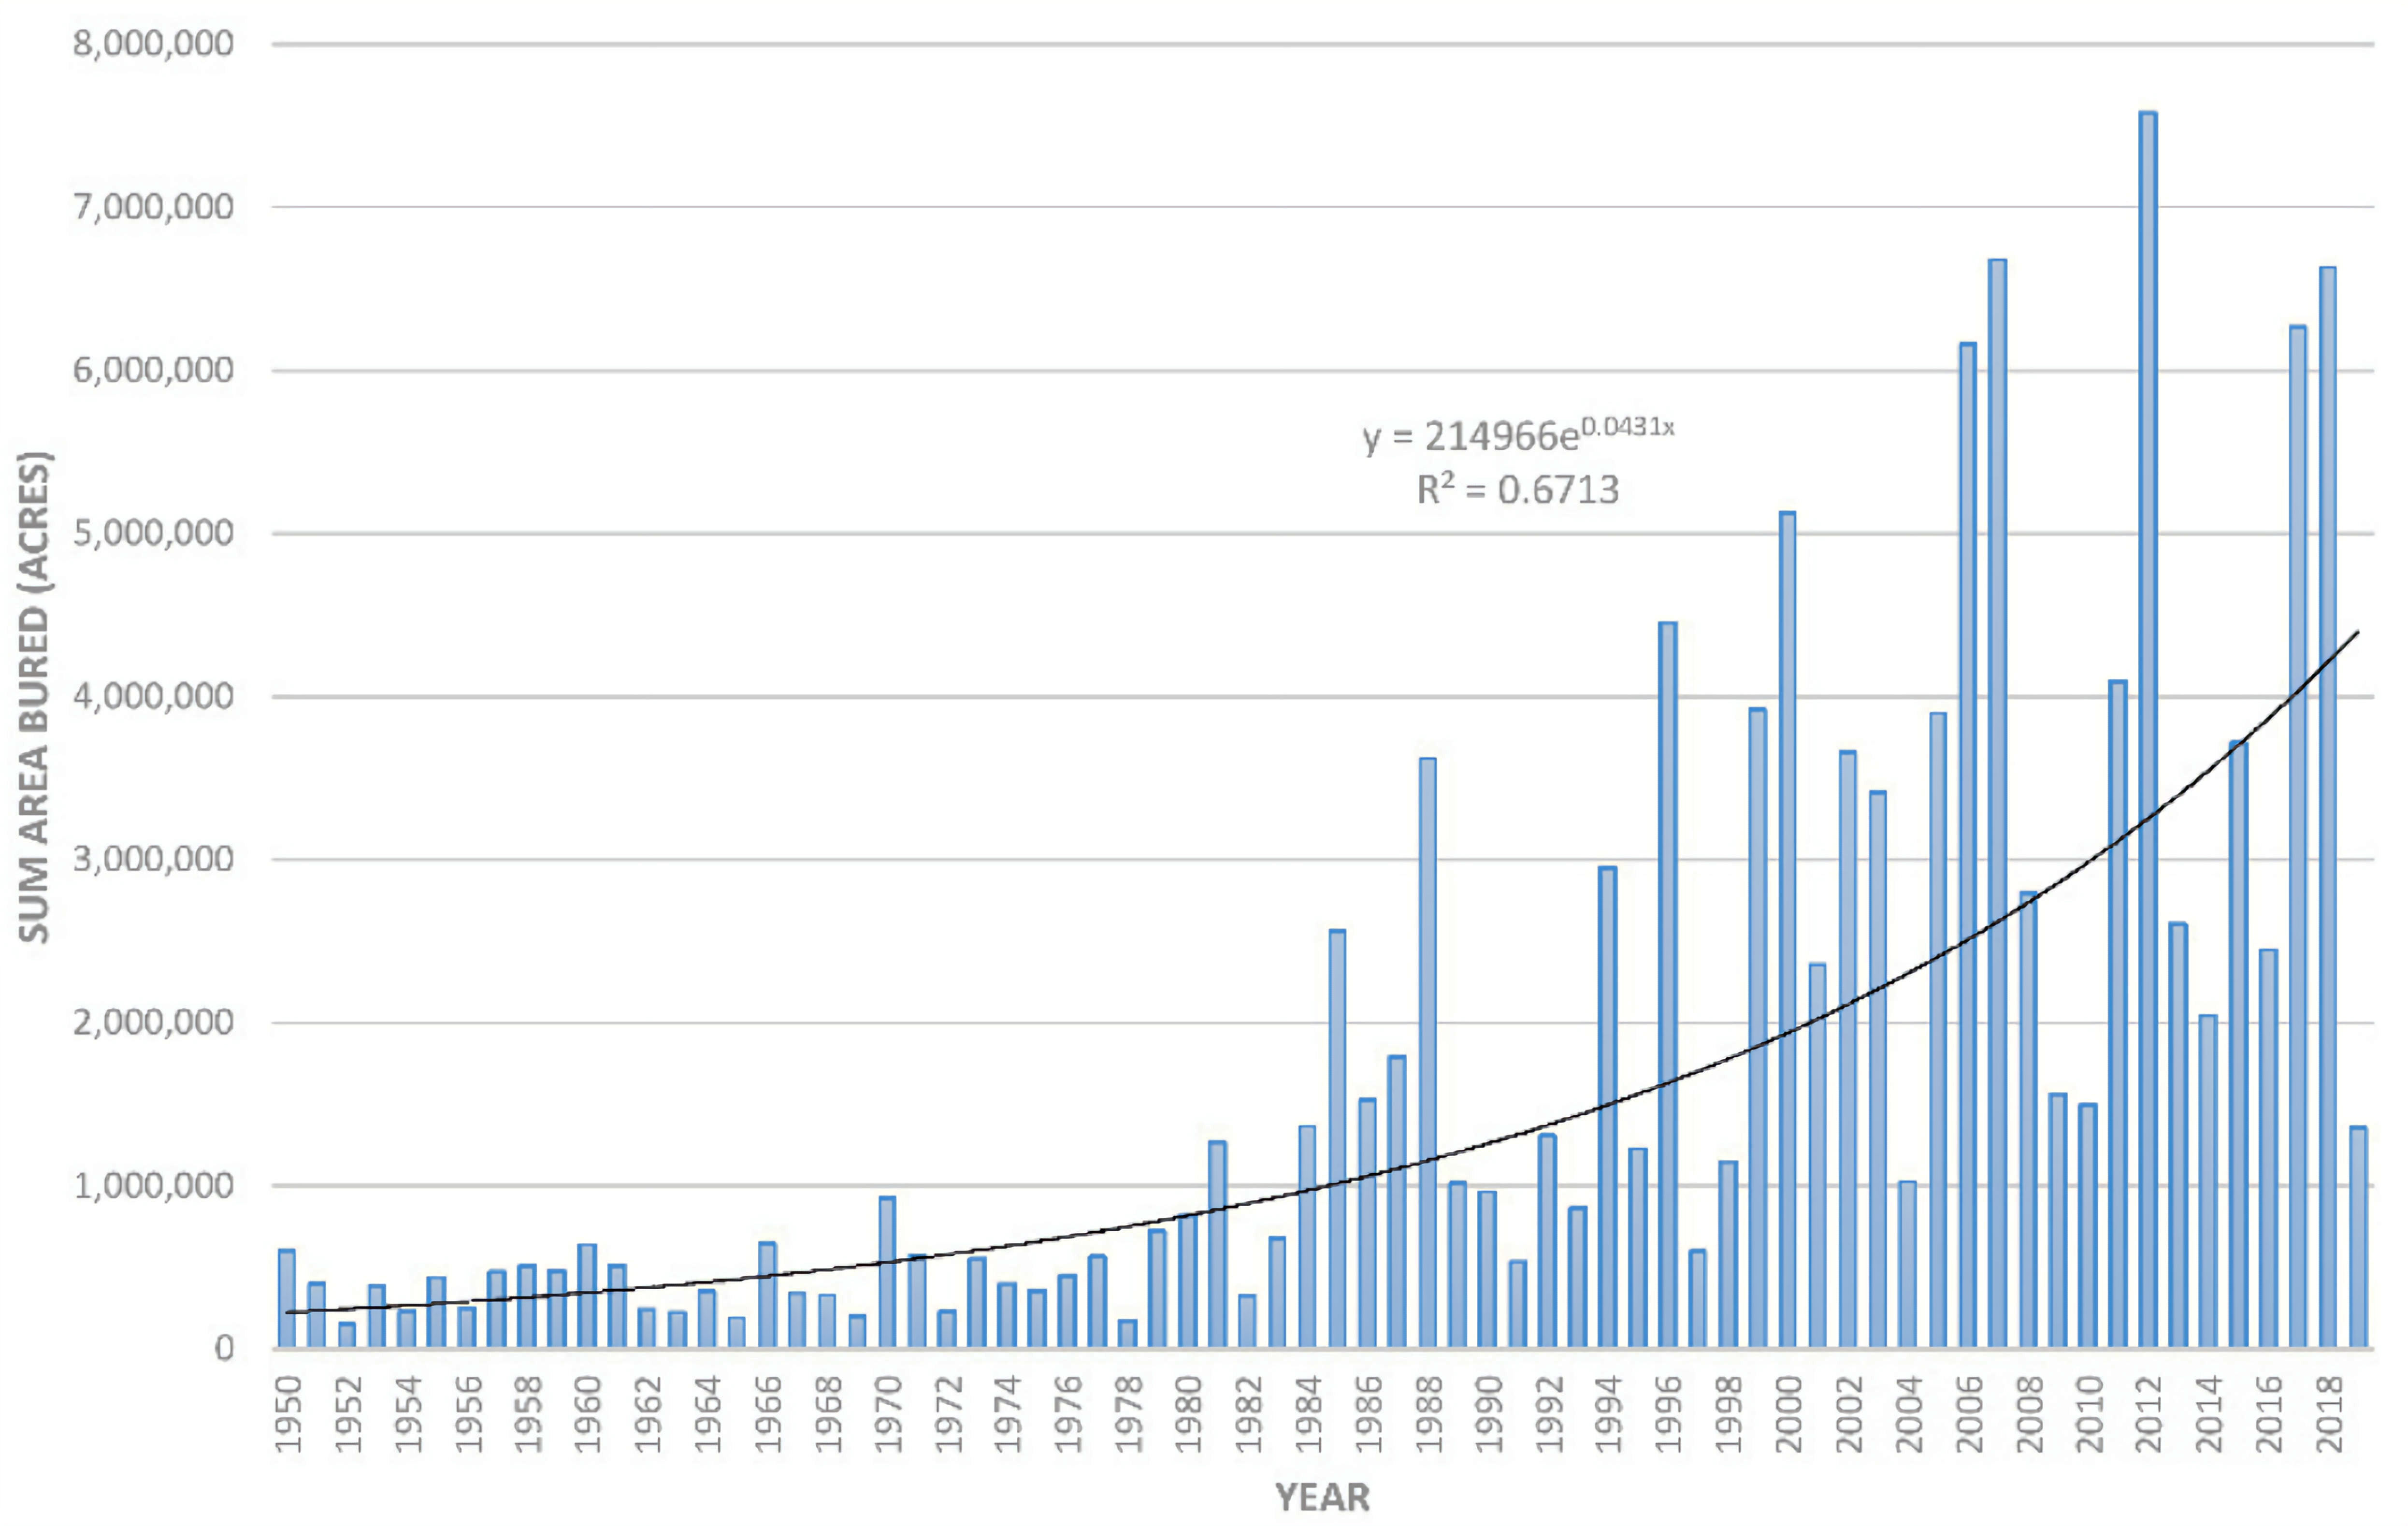
\includegraphics[width=0.9\linewidth]{img/west-usa-area-burned.jpg}
    \caption{The annual total area burned in western United States between 1950 and 2019~\cite{Weber/WildfireTrends}}
    \label{fig:west-usa-area-burned}
\end{figure}

The United Nations call for a radical change in how governments react to wildfires~\cite{UN/FiresReport}.
It is projected that climate change, as well as land-use change, will result in even more frequent and intense wildfires.
By 2050, a global increase in the likelihood of extreme wildfire events of up to $30\%$ can be expected, and even up to $50\%$ by the turn of the century.
Increased drought, high air temperatures, and low humidity, all of which are at least partially caused by the climate change, are classified as dangerous fire weather.
For example, nineteen of the hottest years since 1880 have occurred between the year 2000 and 2022~\cite{NASA/Temperature}.
Such weather is the cause of longer fire seasons, which in turn change the biomass and release more climate-changing carbon and other greenhouse gasses into the atmosphere, resulting in a positive feedback loop.

Spain faces similar difficulties as the rest of the world.
In 2021, the campaign to fight forest fires lasted from the middle of June until the end of October, coinciding with the period of the highest risk of wildfires.
A total of 73 aerial resources were available during the summer campaign~\cite{Spain/Campaign}.
A map of locations of preliminary amphibious airplane deployments for this campaign is shown in Figure~\ref{fig:spain-airplanes-deployment}.
On average, Spain faced approximately 11\,600 wildfires each year in the last decade.
One of the worst wildfires in its history occurred in September of 2021 in the province of Málaga, burning a total of approximately 8\,000 hectares of land.
On the 13th of September, 51 airplanes and helicopters were engaged in aerial firefighting to assist almost a thousand firefighters on the ground~\cite{ElMundo/Malaga}.

\begin{figure}[tb]
    \centering
    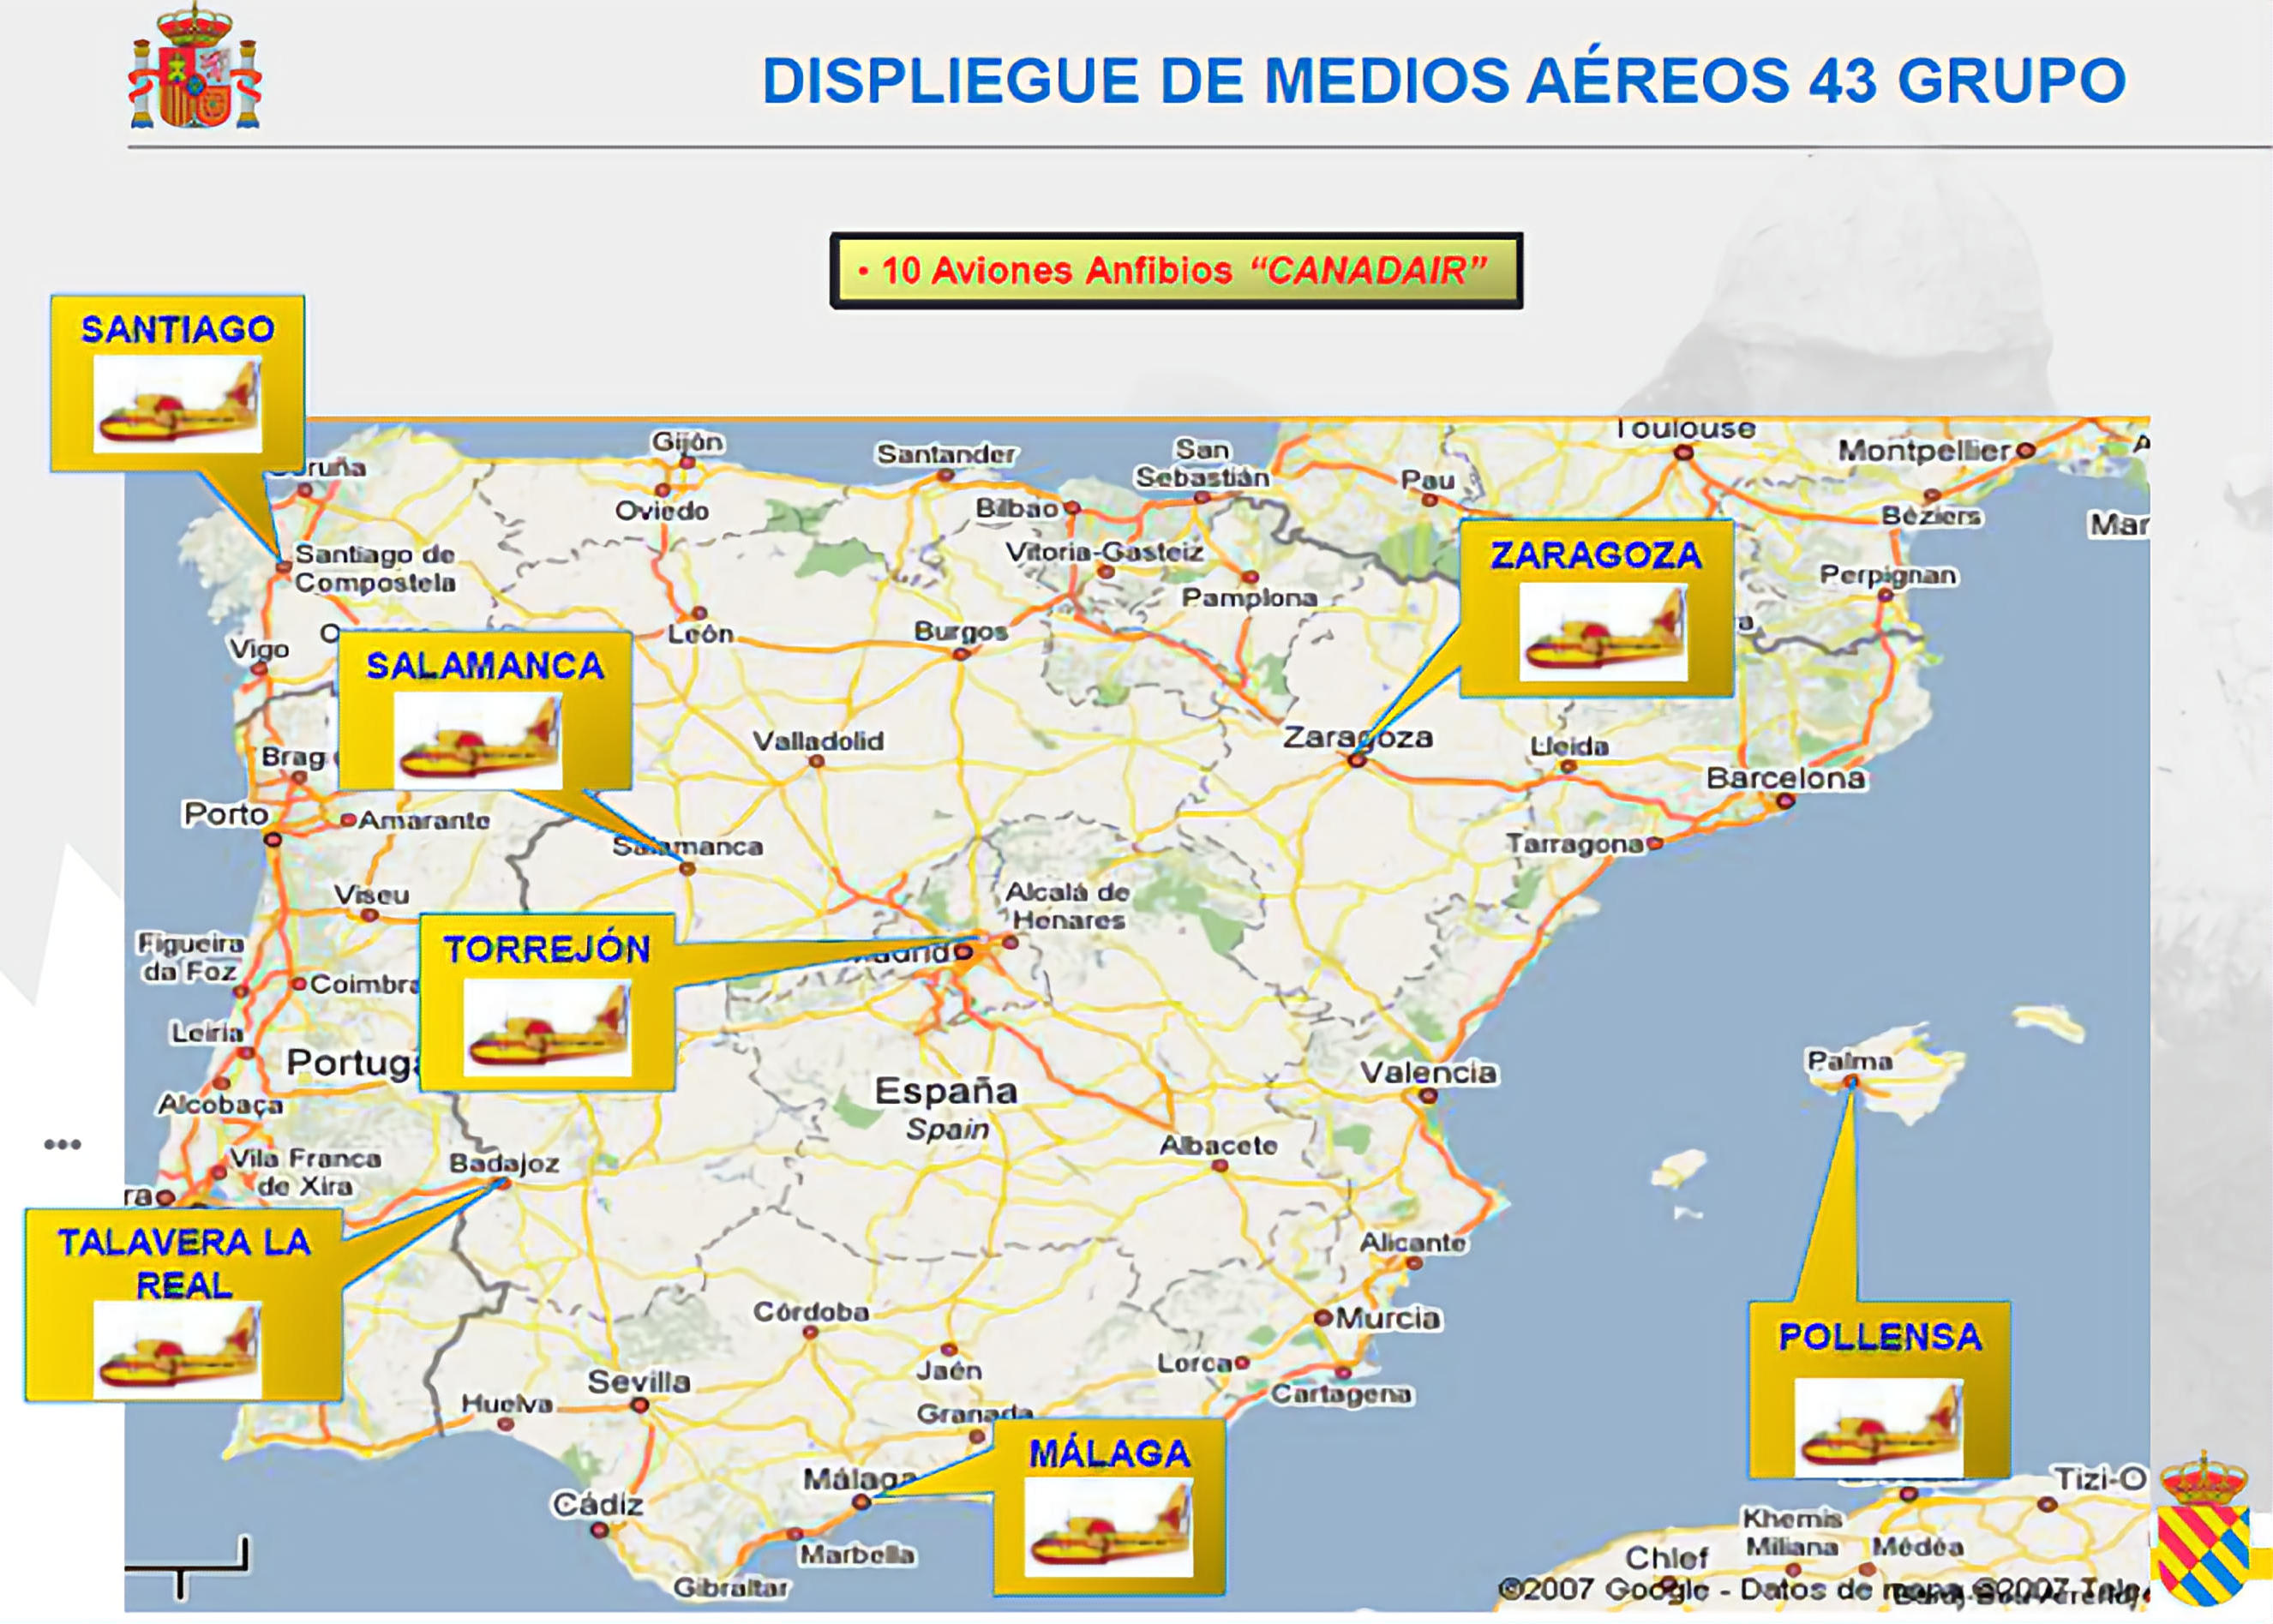
\includegraphics[width=0.9\linewidth]{img/spain-airplanes-deployment.jpg}
    \caption{A map of seaplane deployments in Spain in summer 2021~\cite{Spain/Campaign}}
    \label{fig:spain-airplanes-deployment}
\end{figure}


\section{Aerial Firefighting}

In order to extinguish or control a fire, either fuel, heat, or oxygen must be removed.
Aerial resources are frequently employed to combat wildfires by removing oxygen and heat, in a process called aerial firefighting.
They do not directly extinguish the fire, though, but support the firefighting crews on the ground in their suppression efforts~\cite{Canada/Suppression}.
Airplanes and helicopters drop water or chemical fire retardants near the edge of the burning fire, lowering the air temperature and sometimes creating a barrier between the wildfire and available fuels (firebreak)~\cite{Canada/Retardants}.\footnote{For simplicity, in this paper the term \textit{water} also implies \textit{fire retardants}, \textit{foam}, or any other chemical dropped by aerial resources.}
This allows for ground crews to come closer to the fire and put it out, or improve the created firebreak by removing the fuel (vegetation or other combustible material) with hand tools.

Wildfires of smaller scale are typically tackled in a prompt manner, with dynamic resource scheduling.
On the other hand, large-scale fires require complex protocols and planning models in order to use the available resources to their full potential, shortening the duration of the fire and minimizing the damage to the environment.
Large-scale wildfires typically have more than 20 active aerial resources and can last multiple days, or even weeks.
With such a high number of resources which must be efficiently scheduled arises a need for scalable algorithmic solutions.

This thesis explores a fast heuristic approach for scheduling resources employed in aerial firefighting, along with their assignment to individual areas of the fire, referred to as fire fronts.
The focus is put on extinction of large-scale forest fires, lasting several days.
The model and implementation cater to Spanish regulation of civil aviation~\cite{Spain/AnnexCircular}.
However, with minor changes depending on regulation and other specific requirements, it can be tailored to be applicable for use in other countries.


\section{Performance Goals}

The intended use of the implemented solution is in the planning phase for the next day.
Since aerial firefighting is only performed during the daylight hours, in summer months planning for the following day tends to take place approximately from 22:00 to 24:00.
This allows for a two hour time window in which the implemented algorithm has to find a satisfying solution.
Realistically, it is quite unlikely that the implementation will be run for longer than one hour.
In addition, it is preferable to have a faster variant which could be executed early in the morning in order to improve or modify the found solution in case parameters change (e.g., changes in weather conditions, changes in aircraft or pilot availability, etc.).
The faster variant might also need to be executed during the day for similar reasons.
Ideally, executing the faster variant should not take more than fifteen minutes.

Given these time constraints, it has been decided that, in the scope of this thesis, only one solution will be developed, with a target execution time of under 10 minutes, completely eliminating the need for a second, faster version.
Of course, the exact hardware used to execute the program will have a significant impact on real-world performance, especially if the algorithm benefits from parallelization.
For the purpose of this work, we make the conservative assumption that a mid-range processor (CPU) with four cores will be used, with a moderate amount of system memory (RAM).
That would be the equivalent of an average modern-day laptop.
Moreover, the size of a problem instance has a considerable influence on the time needed to solve it.
We tested the algorithm with a time limit of 10 minutes for large instances of 35 resources and five fire fronts.


\section{Thesis Structure}

This thesis is divided into nine chapters.
The second chapter gives an overview of related literature and existing solutions.
In the third chapter the problem and the model are defined in detail.
The fourth chapter proposes and explains the heuristic algorithm used to solve the problem, and provides the pseudocode.
The fifth chapter focuses on the implementation of the heuristic algorithm in software and elaborates on the formats of input and output data.
The sixth chapter describes which test scenarios were used to evaluate the implementation, and how they were generated.
In the seventh chapter the results are presented and compared with the solutions achieved by integer linear programming.
The eighth chapter proposes changes which could be made in order to improve the quality of the solutions.
The ninth chapter contains the final remarks.
The thesis ends with a list of references, three appendices containing examples of input and output files, and an abstract.

\chapter{Related Work}\label{chap:related-work}

Several models have already been developed with the aim to assist in scheduling different resources for the purpose of maximizing the wildfire suppression.
In~\cite{Veiga/FullScheduler}, Rodríguez-Veiga et~al.\ explore a general integer linear programming model for scheduling both aerial and ground resources, while adhering to Spanish regulations.
They not only minimize the damage caused by the fire, but also the overall cost and the time of resource use.
Planning is done with a time horizon of up to seven hours, and with up to 30 resources.
It is encouraged to repeatedly run the model if a longer time horizon is headed, taking into consideration the changing conditions, instead of setting a longer planning period.
The recommendation is not to exceed a five hour horizon.

In~\cite{Veiga/AerialScheduler}, the authors introduce two integer linear programming models, which schedule only aerial resources, also according to Spanish regulations.
They prioritize minimizing the wildfire containment time and the total flight time.
Two tasks are performed -- assignment of aerial resources to flight routes and assignment to refueling points.
A flight route is determined by the fire front and the water recharge point.
The maximum number of resources that can be present at a water recharge point at one time is taken into consideration, so that the risk of collision is reduced.
Aircraft's capabilities are specified by their carrying capacity and the number of downloads per hour that can be made for each flight route, which is considered to be the same throughout the day.

The authors in~\cite{SkorinKapov/ILP} propose an updated integer linear programming model, focused only on aerial resources and large-scale wildfires.
Note, in a larger fire with several aerial resources, planning and operations of aerial resources require dedicated emergency management~\cite{INFOCACongreso2017}.
Furthermore, the management of aerial operations must be centralized for the entire fire to increase the safety and efficiency of operations.
In the case of Spain, for such fires, the head of aerial operations and the aerial coordinator will assist the incident commander.
Scheduling in~\cite{SkorinKapov/ILP} is performed for an entire day, with up to 35 resources which can perform multiple flights.
Unlike in~\cite{Veiga/AerialScheduler}, they consider the number of downloads per hour for each time slot, to account for changing weather conditions.
They also suggest that, in real scenarios, the lack of fuel is generally not a concern for any base.
Aircraft have enough time to refuel during the mandatory resting periods between flights, meaning that there is no need to perform refueling point optimizations, unlike in~\cite{Veiga/AerialScheduler}. 
Furthermore, they consider that, in reality, several water recharge points are associated with fire fronts ahead of time, removing the need to optimize flight routes.
Contrary to previous papers, they argue that it is not a priority to minimize the monetary costs of large-scale wildfire suppression in the real-time planning phase.
In practice, and particularly for large-scale wildfires, the extinction or incident commander estimates the aerial resources required to keep the fire under control for the next day.
This estimate is qualitative, based on the experience and technical knowledge of both the incident commander and the personnel involved.
Resources are then allocated according to availability.
Note, such decision making is typically independent of cost in this phase, as public safety is the top priority, along with protection of property and natural and cultural resources.
Once the resources are allocated for the next day, they are utilized as best as possible, according to an attack strategy decided by the incident commander and the head of aerial operations.

Lastly, the approach in~\cite{SkorinKapov/ILP} aims to maintain a desired continuity of water flow over all time slots and fire areas.
In practice, the mobilization of resources should be such that continuity of aerial work is achieved over the \textbf{entire} firefighting time period, avoiding intervals with reduced flow of water.
An intense and numerous attack at the beginning of the day may bring the fire temporarily under control, but it may be useless if there are no aerial resources available in the rest of the day~\cite{INFOCACongreso2017}.
Consequently, considering the full day schedule and maintaining continuity of efforts is crucial, even if changes are made dynamically according to the evolution of the fire.   

As described, existing solutions most often use integer linear programming (ILP) in order to create flight schedules for various models.
However, what they all have in common is that they are not scalable.
The authors in~\cite{Veiga/FullScheduler} and~\cite{Veiga/AerialScheduler} only consider a time horizon of several hours, for which they need upwards of 10 minutes to solve when approximately 15 resources are scheduled.
In~\cite{SkorinKapov/ILP}, the authors used a significantly longer planning period, with the execution time of approximately two hours for suboptimal solutions.
Thus, such approaches may not be able to meet the imposed two hour limit when planning for the whole day is needed, not to mention the desired faster version, in many cases.
That is especially true for larger problem instances which more accurately depict real-life efforts to extinguish large-scale wildfires.

The goal of this thesis is to devise and implement an efficient heuristic search algorithm which will drastically decrease the execution time for the model proposed in Ref~\cite{SkorinKapov/ILP}.
While for smaller instances an ILP approach can be desirable as it guarantees the optimal solution is found, for larger instances heuristic solutions are needed.
The heuristic algorithm is meant to complement the existing ILP approach by providing a fast and effective alternative for larger instances.

\chapter{Problem Definition}

\section{Description}

Given various aerial resources and fire fronts, a flight schedule needs to be created, such that the amount of water dropped by aerial resources approaches the target water content as much as possible in every discrete time slot and on every fire front, while at the same time adhering to numerous constraints~\cite{SkorinKapov/ILP}.
The duration of the schedule, exact capabilities of available aerial resources, the distribution of the target water content, etc., are input data for the problem.
In practice, they are determined by the incident commander, based on the current and expected future state of the wildfire, and his assessment.
The output is a complete flight schedule -- a list of all flights with their respective takeoff times and flight paths, i.e., fire fronts to which they are assigned.
It is created for a single day, which is often a part of a multi-day fire suppression effort.
Considering the incredible complexity and interaction of changing weather conditions, unpredictable spread of the fire, and uncertain impacts of suppression efforts, this schedule can only be considered as an estimate that will help in the planning phase of the entire operation.

A large-scale wildfire is often divided into two or more fire fronts (zones), which are handled separately.
During a single flight, an aircraft will work on a single fire front the entire time.
In case of smaller fires, aircraft tend to work in different areas of the fire during a flight as the fire is being extinguished.
However, we focus on large-scale wildfires, where it is common practice for aerial resources to spend a single flight fighting the fire in the same general area, while also maximizing the allowed flight duration.
Each fire front commonly has one or more dedicated water points where aircraft can refill their water tanks, which is predetermined and not a part of the schedule.

Two types of aerial resources are considered: fixed-wing aircraft and rotary-wing aircraft.
Fixed-wing aircraft are referred to simply as \textit{airplanes}, and sometimes as airtankers, water bombers, or amphibious airplanes.
Rotary-wing aircraft are simply called \textit{helicopters}.
A photograph of a fixed-wing aircraft making a drop of water is shown in Figure~\ref{fig:canadair-drop}.

\begin{figure}[tb]
    \centering
    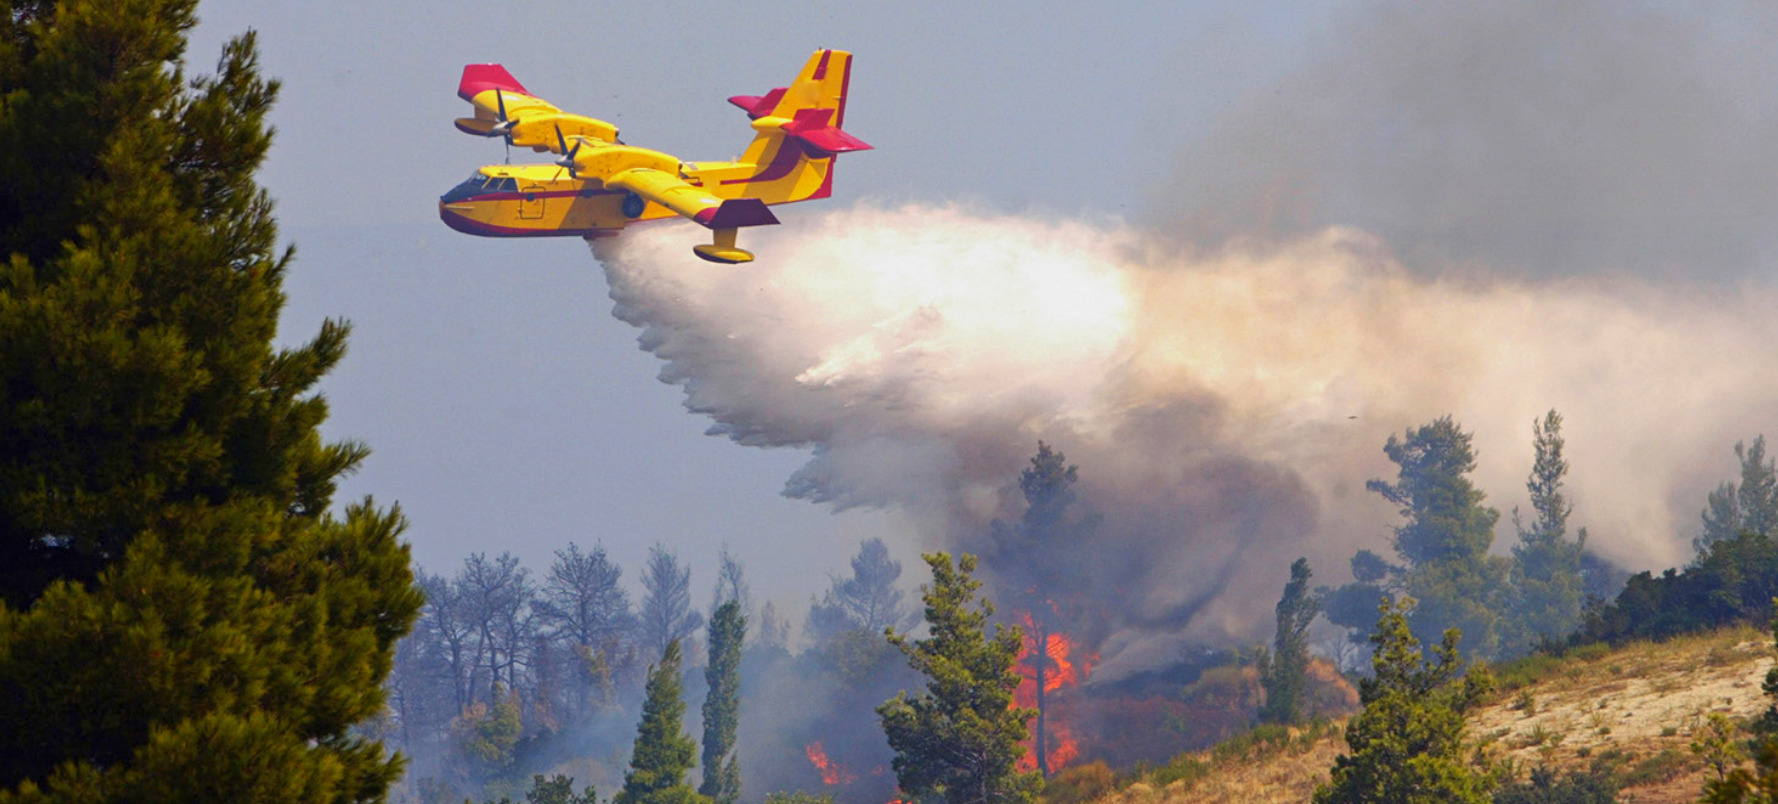
\includegraphics[width=0.95\linewidth]{img/canadair-drop.jpg}
    \caption{An amphibious aircraft dropping water on a wildfire~\cite{Viking/CL415Sheet}}
    \label{fig:canadair-drop}
\end{figure}

In order to model the scheduling problem, we divide the daylight hours into discrete time slots of fixed duration.
Twenty minute increments are selected, because in practice almost every relevant duration is a multiple of 20 minutes.
However, the duration can be easily changed if needed.
In fact, it is implicit -- everything is measured in terms of time slots, and not minutes or hours.

Because time is expressed in discrete time slots, instead of any real value, all decision variables are discrete, too.
The search space is a finite, albeit enormous, set of feasible discrete schedules, and the goal is to find the best one.
Therefore, the task at hand is an NP-hard combinatorial optimization problem.

Once an aircraft arrives at the fire front, it will most likely make multiple drops of water before returning to base.
To do that, it must refill in flight, including before arrival.
Because of their characteristics, helicopters and airplanes refill differently, and have different flight paths and flight speed.
Airplanes refill by scooping from a sufficiently long body of water, shown in Figure~\ref{fig:scooping}, whereas helicopters are often equipped with a bucket which they lower into the water while hovering at a low altitude.
If both types of aircraft were present at the same fire front, airspace coordination would become much more demanding, increasing the odds of an accidental collision.
Therefore, only one type of aircraft may operate at a fire front at the same time.

\begin{figure}[htb]
    \centering
    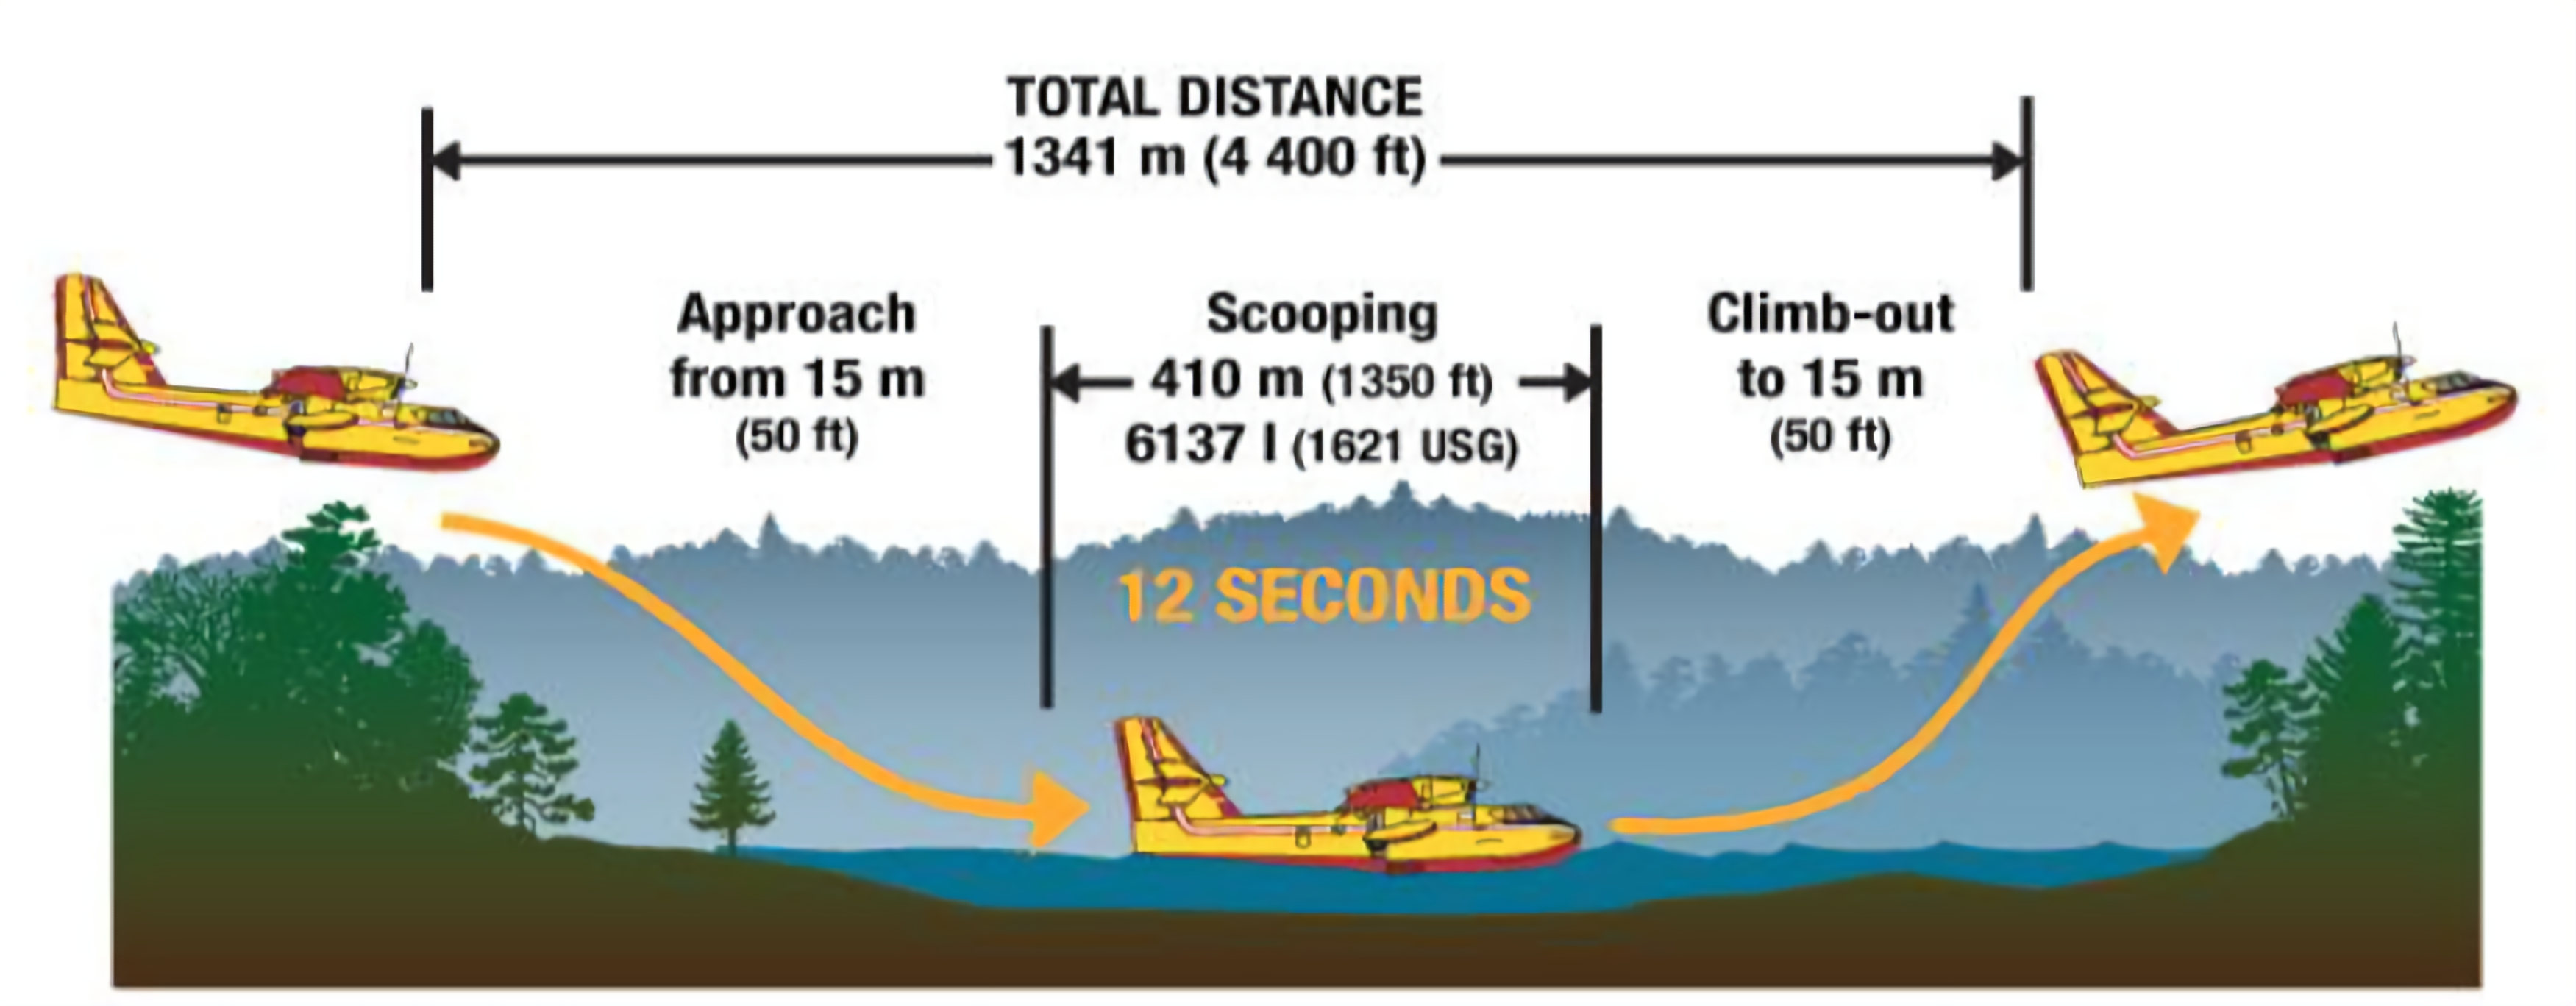
\includegraphics[width=0.95\linewidth]{img/scooping.jpg}
    \caption{An illustration of water scooping by an amphibious aircraft~\cite{Viking/Technique}}
    \label{fig:scooping}
\end{figure}

Helicopters can refill from a small body of water (e.g., a narrow river, a small lake, swimming pools, etc.), whereas airplanes cannot.
If a fire front has only such smaller water points in its vicinity, airplanes will have very limited usability as they will have to make long flights in order to refill at a further, larger water point.
Additionally, if the terrain is generally particularly difficult, it might be inaccessible to airplanes.
Consequently, some fire fronts have restrictions which allow only helicopters to be assigned to those fronts.

When multiple aerial resources are active at the same fire front at the same time, they fly in a carousel-like formation,\footnote{Simply referred to as a \textit{carousel}.} meaning that they are on a very similar flight route, following one another.
The flight route is a circular path defined by the water refilling point, and the discharge point.
An example of a flight route is shown in Figure~\ref{fig:carousel}.
To avoid overcrowding the air space, a limit is set on the number of aerial resources that can fly at the same time at the same front, depending on the fire front.
The limit can depend on the size of the fire front, and the distance and size of the water point.

\begin{figure}[htb]
    \centering
    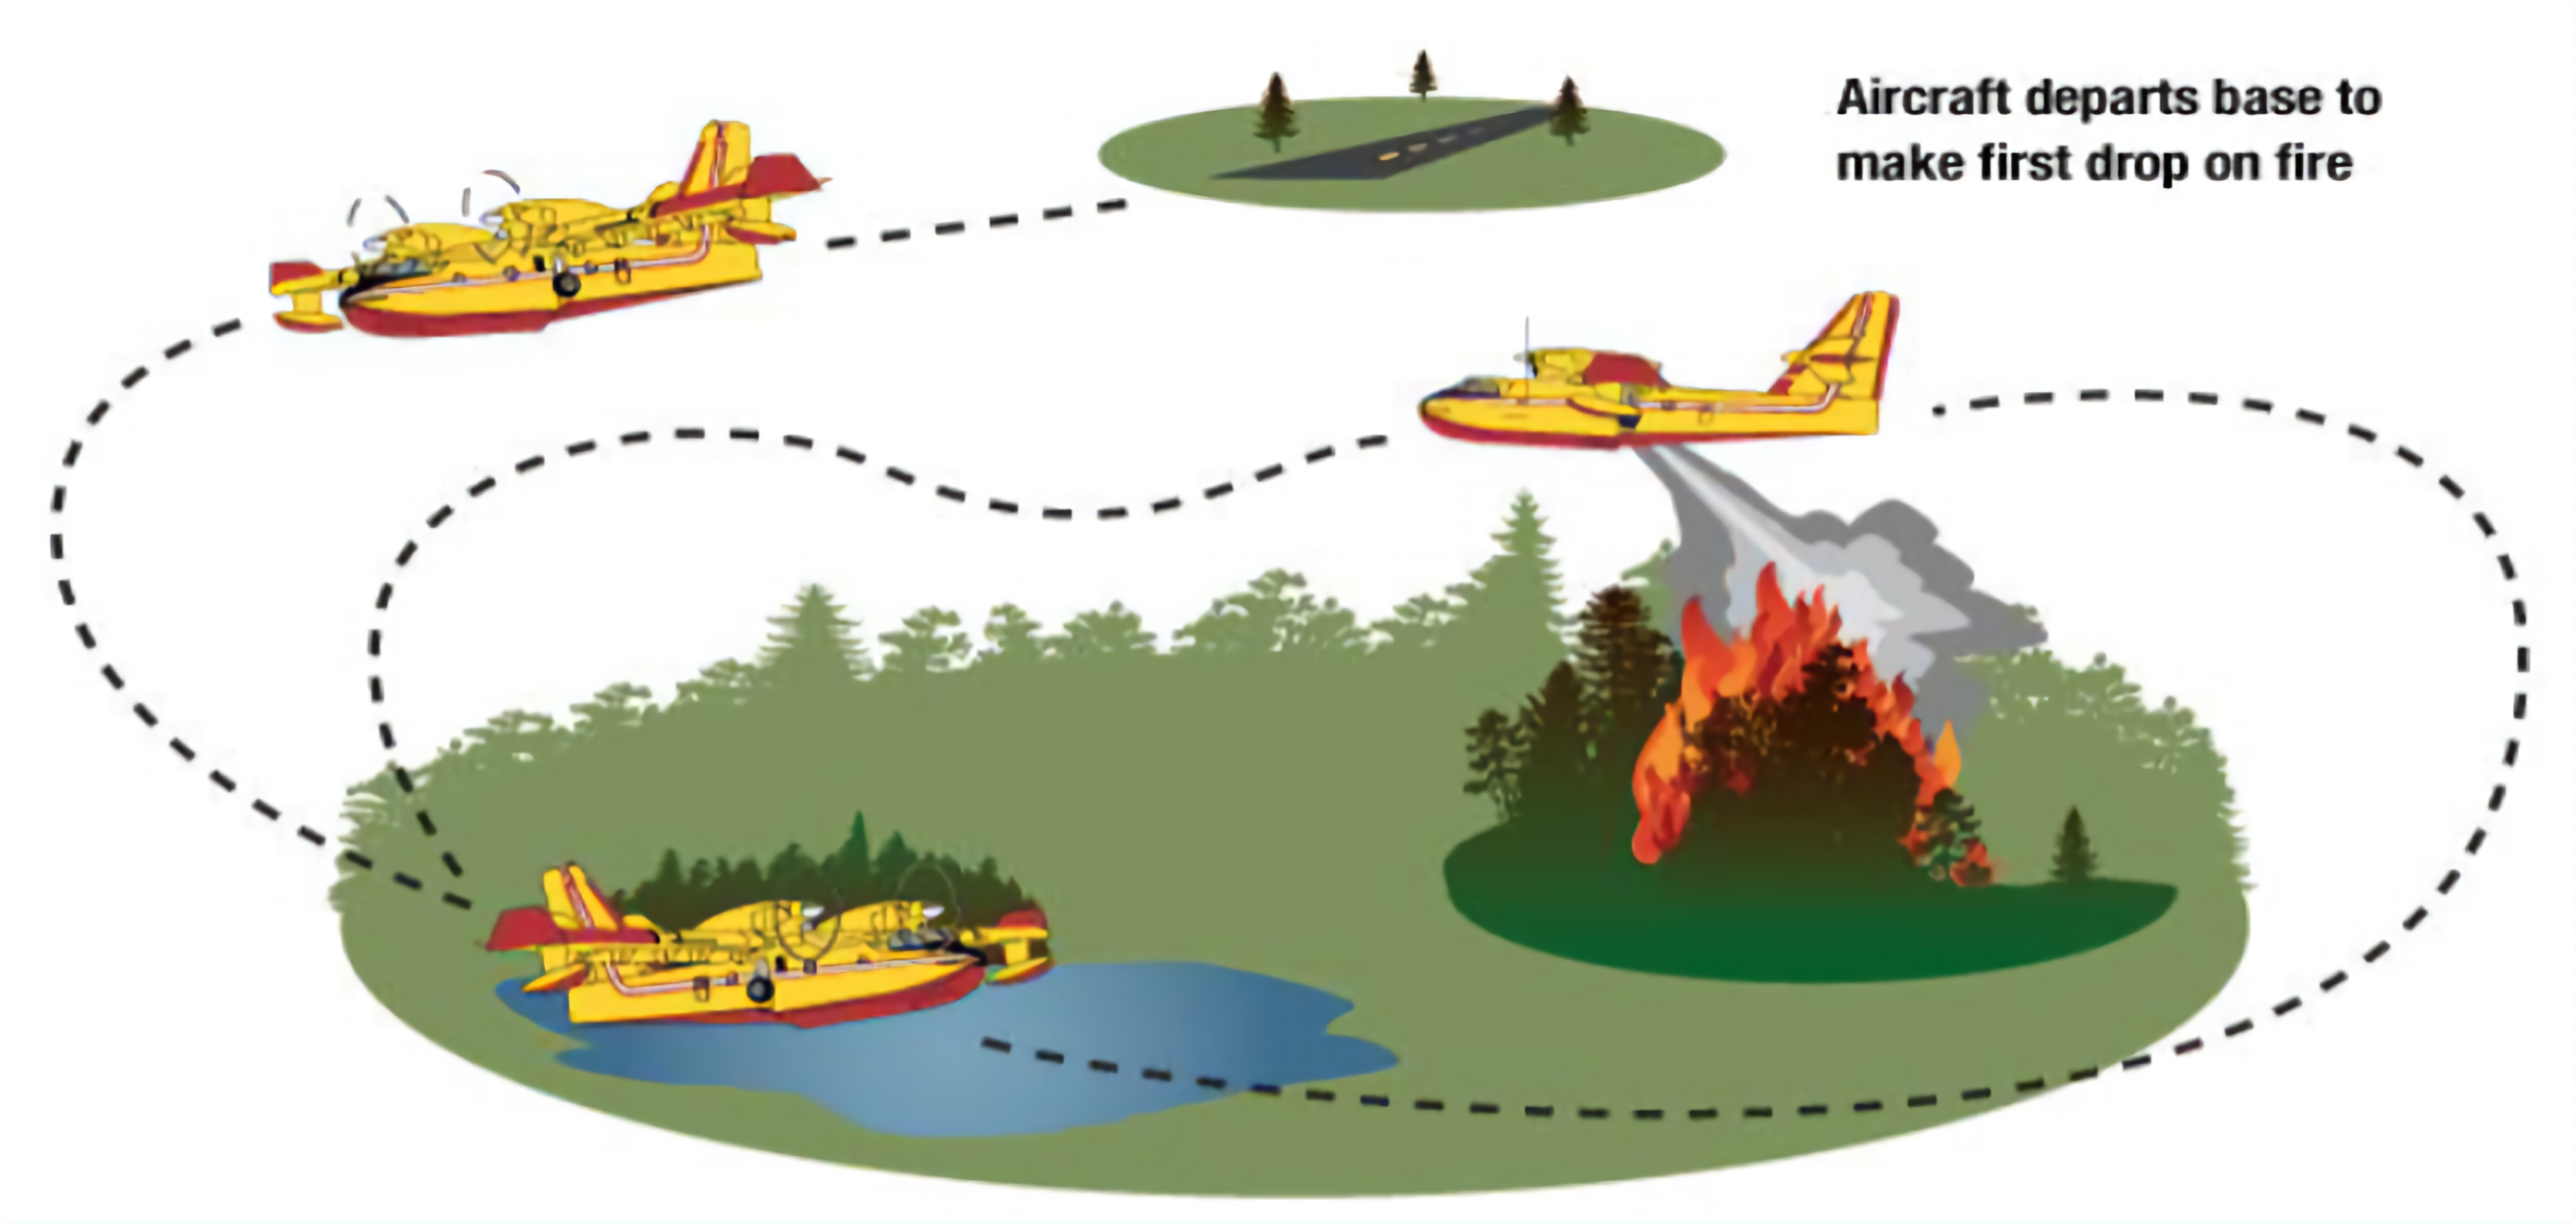
\includegraphics[width=0.95\linewidth]{img/carousel.jpg}
    \caption{A flight path which includes takeoff and repeated filling and dropping of water~\cite{Viking/Technique}}
    \label{fig:carousel}
\end{figure}

Creating a flight schedule cannot be done without taking the pilots (and the rest of the crew) into consideration.
In practice, one flight crew is assigned to one aircraft during a single day, and vice versa.
For that reason there is no need to differentiate between pilots and resources in this model, and whichever rules apply to the crew, also apply to the aircraft.
The terms \textit{aircraft}, \textit{pilot}, and \textit{flight crew} are used interchangeably, with the first being the most common.

Under Spanish regulation, a crew member must not be active for more than 12 consecutive hours~\cite{Spain/AnnexCircular}.
In a special case where the crew consists of military personnel, the 12 hour limit can be extended if resting periods are prolonged.

Between two consecutive flights, the crew must rest and the aircraft must be refueled.
The aircraft is inspected and, if needed, minor repairs can be made during this time.
In this model, we assume all resources will be working properly during availability time slots.
A minimum resting period is prescribed, depending on the duration of the previous flight, and the aircraft type.

Aerial resources are not necessarily available during the entire day.
Airplanes are deployed relatively sparsely, as shown in Figure~\ref{fig:spain-airplanes-deployment}.
On the other hand, helicopters are often readily available in the proximity of the fire, as they require less infrastructure and are overall more common.
In case an airplane was stationed in a faraway base prior to arriving to the general area of the wildfire, it is considered unavailable during the transit.
The same applies when the airplane is returning to another base at the end of the day.
Once the airplane reaches the general area of the wildfire, it is usually stationed in a relatively close base for several days, from where it engages the wildfire.
It is assumed that the mandatory resting period after the transit flight is included in the unavailability period.

Aerial firefighting in itself is significantly more dangerous than flying in normal conditions.
It requires performing special high-risk maneuvers, such as refilling water tanks mid-flight, flying at a low altitude, navigating difficult terrain, or avoiding vertical obstructions like power lines and wind turbines.
Exacerbating factors also include stronger winds, increased temperature, and reduced visibility due to the thick smoke, all caused by the large wildfire.
If we were to add night-time into the equation, the flight would become even more difficult and the risk of an accident would significantly increase.
Therefore, regulations dictate that aerial resources are not permitted to fight fires during night-time hours~\cite{Spain/AnnexCircular}, and the flight schedule is to be created only for the daytime.
While it could be possible for aircraft to perform longer transits at night-time, be it early in the morning or late in the evening, effectively extending the flight schedule, it is not considered in this model.


\section{Phases of Flight}

In each 20-minute time slot, an aerial resource may be active or inactive.
Active resources may be in one of three states:
\begin{itemize}
    \item \textbf{Transit:} travelling to or from the fire front during the entire time slot,
    \item \textbf{Hybrid:} arriving or departing from the fire front during the time slot. The resource spends some time in transit, and some time fighting the fire.
    \item \textbf{Firefighting:} actively fighting the fire during the entire time slot.
\end{itemize}

Consider a flight of duration $T \in \mathbb{N}$ with $u \in \mathbb{N}_0$ transit slots in each direction.
Let the flight begin in time slot $t$.
The previously discussed states correspond to the following time slots (also depicted in Figure~\ref{fig:phases-flight}):
\begin{itemize}
    \item Departing transit time slots: $[ t,\ t + u \rangle$,
    \item First hybrid time slot (arrival at fire): $t + u$,
    \item Firefighting time slots: $[ t + u + 1,\ t + T - u - 1 \rangle$,
    \item Second hybrid time slot (departure from fire): $t + T - u - 1$,
    \item Returning transit time slots: $[t + T - u,\ t + T \rangle$.
\end{itemize}

\begin{table}[htb]
\vspace{0.8\baselineskip}
\centering
\fontsize{9.5pt}{10pt}\selectfont
\begin{tabular}{@{}*5c@{}}
$t~~\cdots~~t+u-1$ & $t+u$ & $t+u+1~~\cdots~~t+T-u-2$ & $t+T-u-1$ & $t+T-u~~~\cdots~~~t+T-1$ \\
\upbracefill & \upbracefill & \upbracefill & \upbracefill & \upbracefill \\
Transit & Hybrid & Firefighting & Hybrid & Transit \\
\end{tabular}
% Faking a Figure, as the illustration is not really a proper table.
\captionof{figure}{Time slot ranges corresponding to different phases of flight} \label{fig:phases-flight}
\end{table}

Some groups of time slots may be empty, depending on parameter values.
If an aircraft is stationed close to a fire front, it is likely that there will be no transit slots, as the aircraft can reach the front within a single time slot.
Helicopters can be stationed at a variety of locations and tend to be within 20 minutes of flight time from the fire~\cite{INFOCACongreso2017}.
Airplanes are required to be stationed at airbases or airports, and typically have longer transit times (e.g., 40 minutes). 
On the other hand, due to the long transit times to and from a distant fire front, it is also technically possible for a flight to have no firefighting time slots.
Such flights are a poor use of available resources, but are not forbidden.
In the exceptional case that the aircraft barely reaches the fire front and already has to start returning to the base in the same time slot, it would be even less efficient than in a regular hybrid time slot.
However, such hybrid slots are not considered in this model, and are treated as if they were a regular hybrid slot.

Aircraft's suppression potential is measured in terms of the number of drops per time slot and fire front.
Note, the number of drops will differ between fronts due to locations of refill points.
Furthermore, they can differ over time due to meteorological conditions affecting flights and refill constraints.
For example, stronger winds may force an aircraft to fly slower, or take a different, longer flight path.
The number of drops is given as a real number, and not an integer, because it represents an estimated average value.
For example, if the value is $1.5$ drops per time slot, the aircraft will likely make one drop in one time slot, and two drops in the other time slot.
The amount of water dropped per time slot is calculated by multiplying the water capacity of the aircraft, with the estimated number of drops per time slot.
All values are given as problem input parameters.

When an aircraft is in a hybrid time slot, it spends some time traveling from the base.
To represent the amount of time spent in transit in such time slots, which depends on the distance from the base to the fire and the current weather conditions, the number of drops per time slot is proportionally smaller compared to a firefighting time slot.


\section{Parameters}

\subsection{Input Parameters}

All problem input parameters, their types and descriptions are listed in Table~\ref{tbl:input-params}.

\begin{table}[htb]
\caption{Descriptions and types of problem input parameters}
\label{tbl:input-params}
\small
\centering
\begin{tabularx}{\hsize}{@{}llX@{}}
Parameter & Type & Description \\
\midrule
$k,\ \mathcal{K}$ & -              & Index and set of aerial resources. \\
$f,\ \mathcal{F}$ & -              & Index and set of fire fronts. \\
$t,\ \mathcal{T}$ & -              & Index and set of consecutive time slots. \\
$V_k$             & $\{0,1\}$      & $1$ if aircraft $k$ is a helicopter, $0$ if it is an airplane. \\
$T_k$             & $\mathbb{N}$   & The flight duration of aircraft $k$, measured in time slots. \\
$R_k$             & $\mathbb{N}$   & The minimum resting period for aircraft $k$, measured in time slots. \\
$N_k$             & $\mathbb{N}$   & The maximum number of flights aircraft $k$ can perform in one day. \\
$P_k$             & $\mathbb{N}$   & The maximum number of continuous time slots in which a pilot is active, including flying and resting time. \\
$A_k^t$           & $\{0,1\}$      & $1$ if aircraft $k$ is available in time slot $t$, $0$ if it is not. \\
$B_{f}$           & $\{0,1\}$      & $1$ if only helicopters can fly on front $f$, $0$ if all types of aircraft can fly on that front. \\
$U_{kf}$          & $\mathbb{N}_0$ & The number of full time slots needed for aircraft $k$ to reach the front $f$. \\
$W_f^t$           & $\mathbb{R}^+$ & The target water content for fire front $f$ in time slot $t$, measured in liters. \\
$S_f$             & $\mathbb{N}$   & The maximum number of resources which can fly at front $f$ at one time. \\
$C_k$             & $\mathbb{N}$   & The water capacity of aircraft $k$, measured in liters. \\
$D_{kf}^t$        & $\mathbb{R}^+$ & The average number of drops aircraft $k$ will make over fire front $f$ in time slot $t$ if it spends the entire time slot actively fighting the fire. \\
$E_{kf}^t$        & $\mathbb{R}^+$ & The average number of drops aircraft $k$ will make over fire front $f$ in time slot $t$ if it is arriving to or leaving the fire front in that time slot. \\
$a_1, a_2, a_3$   & $\mathbb{R}^+$ & The weighting factors used in the objective function (see Section~\ref{sec:objective}). \\
\end{tabularx}
\end{table}


\subsection{Decision Variables}

The flight schedule is unambiguously determined by a takeoff matrix with elements \hbox{$c_{kf}^t \in \left\{ 0, 1 \right\}$}.
If the aircraft $k$ is initiating a flight towards the fire front $f$ in the time slot $t$, the element $c_{kf}^t$ will have value $1$.
Otherwise, the value of $c_{kf}^t$ will be $0$.

Because each aircraft's flights have a predetermined duration $T_k$, the state of each aircraft is known in every time slot solely based on the values of the takeoff matrix.
Consequently, the takeoff matrix is the only necessary decision variable for determining the flight schedule.


\subsection{Auxiliary Variables}

Water surplus in time slot $t$ on fire front $f$ is denoted by the variable $\mathit{WS}_{tf}$.
Water surplus is the difference between the amount of water that was dropped by all resources on that front in that time slot, and the target water content for that time slot and fire front.
If the value is negative, it means that particular target water content was not satisfied.
A positive value indicates that a larger amount of water was dropped than necessary, which is beneficial.

The sum of all water surplus values which are negative is called the negative water surplus, denoted by $\mathit{WS}_n$, and defined in Equation~\ref{eq:wsn-def}.
$\mathit{WS}_n \le 0$ always holds.
\begin{equation}\label{eq:wsn-def}
\mathit{WS}_n = \sum_{t \in \mathcal{T}} \sum_{f \in \mathcal{F}} \min (\!\mathit{WS}_{tf}, 0 )
\end{equation}

The minimal water surplus $Z$ is the smallest water surplus value, defined in Equation~\ref{eq:z-def}.
It may have any real value, but Equation~\ref{eq:z-wsn-relation} always holds.
\begin{equation}\label{eq:z-def}
Z = \min_{\substack{t \in \mathcal{T}\\f \in \mathcal{F}}} \mathit{WS}_{tf}
\end{equation}
\begin{equation}\label{eq:z-wsn-relation}
\mathit{WS}_n = 0 \iff Z \ge 0
\end{equation}

The total water output $\mathit{WO}$ is calculated as the sum of the amount of dropped water over all fire fronts and time slots.
This value is equal to zero if and only if the flight schedule is empty.
Otherwise, the total water output is a positive value.


\section{Objective Function}\label{sec:objective}

The objective function in Equation~\ref{eq:objective} maximizes the weighted sum of three distinct terms, representing three objectives of varying importance, regulated by weighting factors $a_1$, $a_2$, and $a_3$, in that order.
The first term is the sum of negative water surplus over all fire fronts and time slots, which is always negative or equal to zero.
The second term is the minimal water surplus over all fronts and time slots, which may have any real value.
Finally, the third factor is the total water output across all fronts and time slots, which is always non-negative.

\begin{equation}\label{eq:objective}
\max \left( a_1 \cdot \mathit{WS}_n
    + a_2 \cdot Z
    + a_3 \cdot \mathit{WO} \right)
\end{equation}

The original intention was to use the target water content as a hard constraint, meaning any flight schedule which did not meet all targets was unacceptable.
In that scenario, the water surplus would be positive across all fronts and time slots:
\begin{equation}
\mathit{WS}_{tf} \ge 0,\ \forall t \in \mathcal{T},\ \forall f \in \mathcal{F}
\end{equation}
Consequently, the first objective would always be equal to zero for feasible schedules.
Additionally, the second objective would always be positive, meaning the value of the entire objective function would also be positive.

However, meeting the target water content may not be possible, as will be described in detail in Section~\ref{sec:water-distribution}.
In order to solve that issue, meeting the target water content was changed to be a soft constraint, and the concept of maximizing negative water surplus was introduced into the objective function, as shown in Equation~\ref{eq:objective}.
That way schedules which do not meet the targets are penalized, but still considered feasible.

The second term in the objective function is used to facilitate spreading the water surplus more evenly across all time slots and fire fronts.
While other measurements, such as variance of water surplus, could achieve that goal more effectively, using a minimum value keeps the objective function, as well as the entire problem, linear.
It also keeps the model as similar as possible to the one in Ref~\cite{SkorinKapov/ILP}, which is needed for later comparisons of results.

The third term should be considered the least important of the three objectives.
While the total water output is a good measure of how effectively the resources were used in terms of their raw output, it is not indicative of the quality of the suppression efforts.
Dropping a large amount of water on some fronts or time slots, while leaving others neglected, can seriously harm the overall fire suppression.
It is much more beneficial to output less water overall, but in a more uniform manner, especially if the target water content was not met.
That being said, even if some flight does not impact the first or second term, it is still beneficial to schedule it and output more water in total.

Depending on the values of the weights $a_1$, $a_2$, and $a_3$, if the value of the objective function is positive, it is not indicative of the fact that all water content targets have been satisfied.
However, if the value of the objective function is negative, it is certain that the targets have not been fully met.
Of course, it is assumed that all weights are non-negative, as the objective function would not achieve its purpose otherwise.

The total cost, or any equivalent measure, is not considered to be a part of the objective function.
As was previously described, the goal is to maximize the suppression efforts with the given resources, regardless of monetary costs, as is typically done in practice in this phase for large-scale wildfires.
The implicit price limit was already established at the time of provisioning the aerial resources.


\section{Constraints}\label{sec:constraints}

The flight schedule is subject to a number of feasibility and legislative constraints.
Furthermore, some constraints are put in place to simplify the schedule and therefore slightly reduce the search space.
All constraints are listed and explained below.
Constraints apply to every aircraft, unless otherwise specified.

\textbf{Constraint 1.} It is assumed an aircraft cannot change fire fronts during the course of a single flight, which is common practice.
However, a single aircraft may fight the fire on different fronts during different flights in the same day.

\textbf{Constraint 2.} An aircraft is not allowed to take off towards any front before it has returned to base after the previous flight, as well as completed the specified resting period $R_k$ between consecutive flights.
This constraint does not apply to aircraft's first flight of the day as resources are deemed to be refueled and ready to fly immediately at the start of their availability.

\textbf{Constraint 3.} An aircraft is not allowed to be flying before the start of the day, after the end of the day, or during any time slot in which it is marked as unavailable: $A_k^t = 0$.
It is not necessary for the aircraft to complete the resting period before the end of the day or before the start of unavailability.

\textbf{Constraint 4.} An aircraft is not allowed to take off towards a front if it will not be able to make any drops on that front because the front is too far away, i.e., the transit time is too long: $U_{kf} \cdot 2 \ge T_k$.

\textbf{Constraint 5.} The number of times an aircraft takes off must not be greater than the maximum number of flights per day for that aircraft, $N_k$.

\textbf{Constraint 6.} We assume here that all flights last the maximum duration specified by legislation for that aircraft, i.e., stated in the input parameters as $T_k$.
In other words, it is not allowed to perform a shortened flight, for example near the end of the day.
Such an assumption should not reduce suppression efforts since the maximum number of flights $N_k$ is often more restrictive than the forced flight duration.
Although in reality flights can be shorter, in practice, flights tend to be near maximum duration when possible for large-scale ongoing suppression efforts.
Thus, this constraint is used to significantly simplify the model, drastically reducing the solution space.
Furthermore, this assumption eliminates solutions which assign very short flights to resources which may optimize the objective function but is not reasonable or practical from an operational and economic point of view.

\textbf{Constraint 7.} The time span in which an aircraft is active must not be greater than the maximum time a pilot can be present in one day, $P_k$.
More precisely, the active time span is considered to be the time between the beginning of the first flight and the end of the last flight, not including the resting period after the last flight.

\textbf{Constraint 8.} During no time slot may the number of aircraft flying at the same fire front be greater than the maximum number of aircraft allowed at that front, $S_f$, due to limited airspace.
Aircraft flying towards or away from the front, i.e., aircraft in transit, are not counted towards the limit.

\textbf{Constraint 9.} Aircraft of different types cannot fly at the same fire front in the same time slot.
Aircraft in pure transit are not considered in this constraint.

\textbf{Constraint 10.} In case a fire front has restrictions on the type of aircraft that is able to fly at that front ($B_{f} = 1$), aircraft of a different type are not allowed to fly there during any time slot.
Specifically, fire fronts can be limited to only allow helicopters, thus blocking airplane assignments, but not the other way around.

In~\cite{SkorinKapov/ILP}, the authors describe multiple other constraints which were not mentioned in this section.
However, they are primarily used to keep all auxiliary variables in the integer linear programming model in a consistent state, and as such can be considered implementation details and not relevant to our problem definition.

\chapter{Heuristic Algorithm}

Exact methods are algorithms that guarantee an optimal solution to a given problem will be found.
A very crude example is exhaustive (brute-force) search, which systematically enumerates all candidate solutions.
For linear problems, simplex algorithm, interior-point methods, and branch and bound are often used~\cite{HMO/ExactMethods}.
If $\text{P} \neq \text{NP}$, this NP-hard optimization problem cannot be optimally solved in worst-case polynomial time.

When an optimal solution is not required, or the optimization problem is intractable and an exact algorithm cannot solve it in reasonable time, heuristic algorithms may be used.
They do not offer any guarantees with respect to solution quality, but often find satisfying solutions in polynomial time.
Heuristic algorithm are divided into constructive algorithms, which gradually build a solution piece by piece, and improvement algorithms, which start from an existing solution and incrementally improve it~\cite{Cupic/Metaheuristics}.

A metaheuristic algorithm is a kind of general-purpose heuristic algorithm, with the task of guiding problem-specific heuristics towards parts of the solution space which contain high-quality solutions~\cite{Cupic/Metaheuristics}.
They are often inspired by processes occurring in nature.
Examples include tabu search, ant colony optimization algorithms, particle swarm optimization, genetic algorithm, and other evolutionary algorithms.
Metaheuristic algorithms are divided into algorithms which operate on a single solution, and those that operate on a set of solutions (population-based algorithms).

Herein, we describe the heuristic algorithm for aerial resource scheduling proposed in this thesis.


\section{Schedule Representation}

We define a \textit{takeoff} as a 3-tuple consisting of an aerial resource, a fire front, and a time slot, in that order: $(k, f, t)$.
It indicates that the aircraft $k$ is departing in the time slot $t$ in order to fight the fire at the front $f$.
In the pseudocode, a takeoff is typically given the name $e$, short for \textit{element}.

A \textit{schedule} is represented by a set of \textit{takeoffs}.
It is a one-to-one mapping of the model's decision variable, i.e., the takeoff matrix and its elements \hbox{$c_{kf}^t \in \left\{ 0, 1 \right\}$}:
\begin{equation}
    (k, f, t) \in \mathit{Schedule} \iff c_{kf}^t = 1,\ \forall k \in \mathcal{K}, f \in \mathcal{F}, t \in \mathcal{T}
\end{equation}

If a set of takeoffs does not satisfy all the constraints, it is not considered to be a valid schedule.
Because of the way the model and constraints are defined, every subset of a valid schedule is also a valid schedule, including an empty set.
Recall, the water target is a soft constraint moved to the objective function.
Thus, solutions which do not meet the desired water target are considered valid solutions as long as they satisfy the remaining constraints (availability, legislation, etc.). 
Furthermore, once a schedule becomes invalid by adding a takeoff which breaches a constraint, it is impossible to bring it back to a valid state by inserting more takeoffs.
Therefore, we limit ourselves to operating exclusively on valid schedules throughout the heuristic algorithm.
In order for a takeoff to even be considered for insertion into a schedule (referred to as potential or feasible takeoffs), the result must be a valid schedule.

The terms \textit{schedule} and \textit{solution} are used interchangeably.
In the pseudocode, they are sometimes given the short name $s$.

Consider a large problem instance with $7\,000$ different takeoffs, and a maximum of $100$ takeoffs in a schedule.
The upper limit on the number of different schedules is $\binom{7\,000}{100} \approx 1.7 \cdot 10^{226}$.
Obviously, the majority of those schedules are invalid, but that still easily puts the size of the search space above $10^{200}$ different valid solutions.


\section{Greedy Randomized Adaptive Search Procedure}

\begin{algorithm}[tb]
    \caption{Greedy Randomized Adaptive Search Procedure}
    \label{alg:grasp}
    
    \newcommand{\Stemp}{s'}
    \newcommand{\Sbest}{s^{\mathrm{best}}}
    
    \begin{algorithmic}[1]
        \Procedure{GRASP}{$\mathit{iterations}, N_D, N_R, \alpha_G, \alpha_D, \alpha_R, k_{r, G}, k_{p, G}, k_{r, R}, k_{p, R}, T_0, \beta, L$}
            \State $\Sbest \gets \emptyset$\,;
            \For{$i \gets 1$ \textbf{to} $\mathit{iterations}$} \label{alg:grasp-line-for-loop}
                \State $s \gets$ \Call{ConstructGreedySolution}{$\alpha_G, k_{r, G}, k_{p, G}$};
                \State $\Stemp \gets$ \Call{LocalSearch}{$s, N_D, N_R, \alpha_D, \alpha_R, k_{r, R}, k_{p, R}, T_0, \beta, L$};
                \If{$f(\Stemp) > f(\Sbest)$} \label{alg:grasp-line-if-better}
                    \State $\Sbest \gets \Stemp$;
                \EndIf
            \EndFor
            \State \textbf{return} $\Sbest$;
        \EndProcedure
    \end{algorithmic}
\end{algorithm}

The \textit{greedy randomized adaptive search procedure} (GRASP) is a multi-start metaheuristic algorithm, first introduced in Ref~\cite{Feo/GraspFirst}.
Each iteration or independent start consists of two phases -- initial construction, and local search~\cite{Feo/GraspReview}.
The construction phase employs a randomized greedy approach which most often starts with an empty solution.
Local search is then applied to improve upon the initial solution.
The two phases are otherwise not related, and exact algorithms for each phase can be chosen and modified practically without restrictions.
However, the search is required to be stochastic, as there is no sense in executing a deterministic algorithm more than once.
In the proposed algorithm, both phases are stochastic.

The GRASP pseudocode is shown in Algorithm~\ref{alg:grasp}.
The function takes a large number of parameters, all of which will be explained in later sections, where they are used.

Because of complicated constraints, especially the one stating that different types of aircraft cannot fly at the same front at the same time, it is easy for the search to drift in a certain direction and end up with parts of the solution that hardly ever change.
As an example, some schedule might have only airplanes flying at the fire front $f$ during the first half of the day, when it would have been better for them to be flying at a different front, or at $f$ but in the afternoon.
Making such a switch during local search can be extremely unlikely, particularly if it was not considered when designing the algorithm.
GRASP is the metaheuristic of choice because restarting the search often leads to vastly different initial solutions, some of which will hopefully nudge local search in a different direction.
Moreover, it can be seen that iterations have no search memory, making them almost completely independent from one another, except for the result aggregation phase (line~\ref{alg:grasp-line-if-better}).
This makes the algorithm trivially parallelizable, which is another reason why GRASP was selected.


\section{Randomized Greedy Algorithm}

\begin{algorithm}[tbp]
    \caption{Greedy Solution Construction}
    \label{alg:greedy}
    
    \newcommand{\Solution}{\mathit{Solution}}
    
    \begin{algorithmic}[1]
        \Procedure{ConstructGreedySolution}{$\alpha_G, k_{r, G}, k_{p, G}$}
            \State $\Solution \gets \emptyset$\,;
            \State $C \gets$ Candidate set of all feasible takeoffs in $\Solution$;
            \While{$C \not= \emptyset$} \label{alg:greedy-line-while-nonempty}
                \State $\Solution \gets$ \Call{GreedilyInsertTakeoff}{$\Solution, \alpha_G, k_{r, G}, k_{p, G}$};
                \State Update $C$ with respect to constraints;
            \EndWhile
            \State \textbf{return} $\Solution$;
        \EndProcedure

        \State

        \Procedure{GreedilyInsertTakeoff}{$s, \alpha_G, k_r, k_p$}
            \State $\Solution \gets s$;
            \State $C \gets$ Candidate set of all feasible takeoffs in $\Solution$;
            \If{$C = \emptyset$} \label{alg:greedy-line-check-empty}
                \State \textbf{return} $\Solution$;
            \EndIf

            \State $o(e) \gets$ Objective function value for $\Solution \cup \{ e \}$; \label{alg:greedy-line-o-def}

            \State $r(e) = \left\vert \left\{ e' \in C \, \mid \, e'.k = e.k \right\} \right\vert$; \label{alg:greedy-line-r-def}

            \State Calculate available takeoffs if $e$ were chosen next: $C_e$ for all $e \in C$;
            \State $p(e) = \left\vert C_e \right\vert$ for all $e \in C$; \label{alg:greedy-line-p-def}
            
            \State Evaluate $o(e)$, $r(e)$, $p(e)$ for all $e \in C$;

            \State $\hat{o} \gets$ Linearly scaled $o$ to range $\left[ 0, 1 \right]$;
            \State $\hat{r} \gets$ Linearly scaled $r$ to range $\left[ 0, 1 \right]$;
            \State $\hat{p} \gets$ Linearly scaled $p$ to range $\left[ 0, 1 \right]$;

            \State Evaluate the fitness function:
            \State ~~~~$f(e) = \hat{o}(e) - k_r \cdot \hat{r}(e) + k_p \cdot \hat{p}(e)$ for all $e \in C$; \label{alg:greedy-line-fitness-def}

            \State $\mathit{f^{min}} \gets \min \{f(e) \, \mid \, e \in C \}$;
            \State $\mathit{f^{max}} \gets \max \{f(e) \, \mid \, e \in C \}$;
            \State $\mathit{RCL} \gets \left\{e \in C \, \mid \, f(e) \ge f^{max} - \alpha_G \left( f^{max} - f^{min} \right) \right\}$; \label{alg:greedy-line-rcl}
            \State Randomly select $\mathit{Takeoff}$ from $\mathit{RCL}$;

            \State $\Solution \gets \Solution \cup \{ \mathit{Takeoff} \}$;
            \State \textbf{return} $\Solution$;
        \EndProcedure
    \end{algorithmic}
\end{algorithm}

A randomized greedy algorithm is used in the first phase of GRASP.
Its pseudocode is given in Algorithm~\ref{alg:greedy}.
It is a constructive algorithm, meaning that it starts from an empty solution and gradually inserts elements into it.
Construction stops when there are no more elements which can be inserted (line~\ref{alg:greedy-line-while-nonempty}).

The element to be inserted in each iteration is randomly chosen from a \textit{restricted candidate list} (RCL), a concept first described in Ref~\cite{Hart/RCL}.
All candidate elements, i.e., feasible takeoffs, are evaluated based on a fitness function.
A threshold is calculated based on the value of the parameter \hbox{$\alpha_G \in [ 0, 1 ]$}, as shown in line~\ref{alg:greedy-line-rcl}.
Because we are dealing with a maximization problem, only the takeoffs with the fitness value higher or equal to the threshold enter the restricted candidate list.
If the value of $\alpha_G$ is $0$, the best takeoff is selected every time, and the algorithm is completely deterministic.
If the value is $1$, the selection is completely random.

Instead of using the parameter $\alpha_G$ and the threshold, the RCL could be defined by taking a predefined number of elements with the highest fitness value.
It was decided not to use this approach because the quality of the solution can vary quite a lot for instances of different sizes if the same number is used.
For example, picking ten elements out of a thousand can be too restrictive, while picking ten out of twenty can be too random.
On the other hand, selecting the best $5\%$ of elements ($\alpha_G = 0.05$) should give mostly consistent results regardless of instance size.

The fitness function $f(e)$ is not the same as the objective function.
Instead, a weighted combination of three metrics is used in order to measure the benefit of selecting each takeoff.
The metrics are designed so that the choice of a takeoff in one iteration does not severely limit the choices available in the subsequent iteration, which is effectively limiting the greediness.

The first metric $o(e)$ (line~\ref{alg:greedy-line-o-def}) calculates the value of the objective function for the solution if takeoff $e$ were inserted.
It does not have an explicit weighting factor associated with it, as it is considered to be a baseline with the implicit factor $1$.

The second metric is the function $r(e)$, defined in line~\ref{alg:greedy-line-r-def}.
It counts the number of distinct potential takeoffs for the same aerial resource as the one in takeoff $e$.
Takeoffs with a lower value are preferred because related aircraft have fewer takeoffs left to choose from.
In later stages the choice will probably be further reduced, as other inserted takeoffs might block previously available takeoffs.
The value is scaled by a non-negative weighting factor $k_r \in \mathbb{R}^+$.

The third metric is $p(e)$ (line~\ref{alg:greedy-line-p-def}), used to count what would be the total number of feasible takeoffs in the next iteration if takeoff $e$ were selected in this iteration.
Higher values are considered better because they mean selecting that takeoff makes less of a difference with respect to limiting the number of choices in the future.
The value is scaled by a non-negative weighting factor $k_p \in \mathbb{R}^+$.

In order to avoid issues with different scales of different metrics, each of them is scaled to the range $[0, 1]$.
The importance of a metric is then determined only by the assigned weighting factor.
All of the metric are combined into the fitness function in line~\ref{alg:greedy-line-fitness-def}.

The candidate takeoffs need to be re-evaluated in every iteration because the benefits associated with every takeoff change when another is added to the solution.
The candidate set can also drastically change, as the insertion of one takeoff can make dozens of others infeasible.

The check in line~\ref{alg:greedy-line-check-empty} is redundant in the construction phase because of the condition in line~\ref{alg:greedy-line-while-nonempty}.
However, it will be relevant when the same procedure is reused as a part of local search is Section~\ref{sec:repair}.


\section{Local Search}

\textit{Local search} (LS) aims to improve the solution previously found during the greedy construction phase.
It is an improvement algorithm, meaning that it starts with a valid solution and iteratively attempts to find another solution with a higher objective function value, usually stopping when a local optimum is found~\cite{Feo/GraspReview}.
A solution is locally optimal if there is no other solution in the neighborhood with a higher value of the objective function (for a maximization problem).
A neighborhood of a solution is the set of valid solutions which can be reached from the current solution by performing a \textit{move} operation~\cite{Cupic/Metaheuristics}.
The design of those operations plays a vital role in the performance of the algorithm.

The pseudocode is given in Algorithm~\ref{alg:localsearch}.
In the proposed heuristic algorithm, local search is implemented as a combination of large neighborhood search and simulated annealing.
Large neighborhood search is used to sample a single solution $s'$ from the neighborhood (lines~\ref{alg:localsearch-line-destroy} and \ref{alg:localsearch-line-repair}).
Simulated annealing is then used to determine if the sampled solution should be accepted as the current solution $s$ (lines~\ref{alg:localsearch-line-sa-start}~--~\ref{alg:localsearch-line-sa-end}).
Both algorithms are explained in detail in upcoming sections.
Every sampled solution $s'$ is compared to the incumbent solution $s^{\mathrm{best}}$ (line~\ref{alg:localsearch-line-if-best}), which is updated if necessary.

There can be a number of different reasons why the search would be terminated, commonly named stopping criteria.
For example, the time limit is exceeded, the number of iterations without improvement of the incumbent solution is reached, or a local optimum is found.
Because the neighborhood is not exhaustively searched in this version of local search, it is not possible to say with certainty if a local optimum was reached.
Instead, the search is stopped when the total number of iterations, $L$, is reached.

\begin{algorithm}[tb]
    \caption{Local Search}
    \label{alg:localsearch}
    
    \newcommand{\Stemp}{s'}
    \newcommand{\Sbest}{s^{\mathrm{best}}}
    
    \begin{algorithmic}[1]
        \Procedure{LocalSearch}{$s, N_D, N_R, \alpha_D, \alpha_R, k_{r, R}, k_{p, R}, T_0, \beta, L$}
            \State $\Sbest \gets s$;
            \State $T \gets T_0$; \label{alg:localsearch-line-temp-init}
            \For{$i \gets 1$ \textbf{to} $L$}
                \State $s_D \gets$ \Call{Destroy}{$s, N_D, \alpha_D$}; \label{alg:localsearch-line-destroy}
                \State $\Stemp \gets$ \Call{Repair}{$s_D, N_R, \alpha_R, k_{r, R}, k_{p, R}$}; \label{alg:localsearch-line-repair}
                \If{$f(\Stemp) > f(\Sbest)$} \label{alg:localsearch-line-if-best}
                    \State $\Sbest \gets \Stemp$;
                \EndIf
                
                \State $\Delta f =  f(\Stemp) - f(s)$; \label{alg:localsearch-line-sa-start}
                \If{$\Delta f > 0$\, \textbf{or}\, $\mathrm{rand}(0, 1) < e ^ {\Delta f / \, T}$} \label{alg:localsearch-line-sa-accept}
                    \State $s \gets \Stemp$;
                \EndIf
                
                \State $T \gets \beta \cdot T$; \label{alg:localsearch-line-sa-end}
            \EndFor
            \State \textbf{return} $\Sbest$;
        \EndProcedure
    \end{algorithmic}
\end{algorithm}


\section{Large Neighborhood Search}

\textit{Large neighborhood search} (LNS) is a metaheuristic algorithm, proposed for the first time in Ref~\cite{Shaw/LNS}.
It belongs to a class of \textit{very large-scale neighborhood search} (VLSN) heuristic algorithms, which are based on empirical evidence that algorithms exploring larger neighborhoods tend to find solutions of higher quality.
Obviously, thoroughly exploring a larger neighborhood comes at a significant computational cost which may render such an algorithm practically unusable.
Large neighborhood search approaches this problem by using an implicit neighborhood which can be stochastically sampled~\cite{Pisinger/LNS}.
The neighborhood is defined by a pair of \textit{destroy} and \textit{repair} methods.
The \textit{destroy} method takes a feasible solution and, usually in some heuristic manner, destroys parts of it.
The resulting partial solution, which may or may not be feasible, is passed to the \textit{repair} method to be reconstructed and made feasible, but different from the starting solution.
Reconstruction can also be done heuristically, although this is not mandatory.

It can be concluded that the neighborhood of a solution is the set of all solutions which can be reached by applying the \textit{destroy} and \textit{repair} methods.
Considering the methods' stochastic nature and neighborhood size, it is highly unlikely that the same neighbor would be generated multiple times, even if the neighborhood were sampled many times over.
One can sample any number of neighbors from the implicit neighborhood, for example to choose the best one out of the sampled subset. 
However, in this heuristic algorithm it was chosen to generate a single neighbor, for reasons which are explained in Section~\ref{sec:simulated-annealing}.


\subsection{Destroy Method}

The pseudocode of the \textit{destroy} method is shown in Algorithm~\ref{alg:destroy}.
The solution is partially destroyed by removing up to $N_D$ takeoffs.
While it is theoretically possible that the solution contains fewer than $N_D$ takeoffs, destroying all of them would result in an empty solution, which defeats the purpose of an iterative search algorithm.
The solution remains feasible throughout this method.

Takeoffs are ranked based on their contribution to the solution quality.
That is measured by calculating the objective function value of the solution without a takeoff, as defined by the function $f$ in line~\ref{alg:destroy-line-f-def}.
The best takeoff is the one with the lowest value of $f$, meaning that it was critical in increasing the objective function value.

From rudimentary testing it was concluded that removing the best or the worst takeoff yields significantly worse results than if it were chosen completely at random.
It was also concluded that randomly choosing a takeoff from a subset of best takeoffs gives lower quality solutions than choosing it from a subset of worst takeoffs.
Therefore, a design choice was made to use the restricted candidate list shown in line~\ref{alg:destroy-line-rcl}, similar to the RCL used in the greedy construction algorithm.
This way, a takeoff is chosen from a subset of worst takeoffs, with the possibility to control the randomness via the parameter $\alpha_D$.
When $\alpha_D$ is set to $1$, the takeoff is chosen completely at random.

In order to get a sense of scale, let us consider a solution $s$ with $100$ takeoffs, and $N_D = 5$, both of which are realistic values for larger problem instances.
The described method can destroy the solution in $\binom{\vert s \vert}{N_D} = \binom{100}{5} \approx 7.5 \cdot 10^7$ different ways, resulting in the same number of partial solutions.
However, the neighborhood size is much larger than that, because each of those partial solution can then be repaired in thousands, and often millions, of different ways.

\begin{algorithm}[htbp]
    \caption{Destroy Method}
    \label{alg:destroy}
    
    \newcommand{\Solution}{\mathit{Solution}}
    
    \begin{algorithmic}[1]
        \Procedure{Destroy}{$s, N_D, \alpha_D$}
            \State $\Solution \gets s$;
            \State $N'_D \gets \min ( N_D, \vert s \vert )$;
            
            \For{$i \gets 1$ \textbf{to} $N'_D$}
                \State $f(e) \gets$ Objective function value for $\Solution \setminus \{ e \}$; \label{alg:destroy-line-f-def}
                \State Evaluate $f(e)$ for all $e \in \Solution$;
                
                \State $\mathit{f^{min}} \gets \min \{f(e) \, \mid \, e \in \Solution \}$;
                \State $\mathit{f^{max}} \gets \max \{f(e) \, \mid \, e \in \Solution \}$;
                \State $\mathit{RCL} \gets \left\{e \in \Solution \, \mid \, f(e) \ge f^{max} - \alpha_D \left( f^{max} - f^{min} \right) \right\}$; \label{alg:destroy-line-rcl}
                \State Randomly select $\mathit{Takeoff}$ from $\mathit{RCL}$;
                
                \State $\Solution \gets \Solution \setminus \{ \mathit{Takeoff} \}$;
            \EndFor
            \State \textbf{return} $\Solution$;
        \EndProcedure
    \end{algorithmic}
\end{algorithm}


\subsection{Repair Method}\label{sec:repair}

\begin{algorithm}[tb]
    \caption{Repair Method}
    \label{alg:repair}

    \newcommand{\Stemp}{s'}
    \newcommand{\Sbest}{s^{\mathrm{best}}}
    \newcommand{\Solution}{\mathit{Solution}}

    \begin{algorithmic}[1]
        \Procedure{OptimalDFS}{$s, V$}
            \State $\Sbest \gets s$;
            \State $C \gets$ Candidate set of all feasible takeoffs in $s$;

            \ForAll{$e \in C \setminus V$} \label{alg:repair-line-remove-visited}
                \State $V' \gets V$;
                \State $\Stemp \gets$ \Call{OptimalDFS}{$s \cup \{ e \}, V'$}; \label{alg:repair-line-recursion}
                \If{$f(\Stemp) > f(\Sbest)$}
                    \State $\Sbest \gets \Stemp$;
                \EndIf
                \State $V \gets V \cup \{ e \}$;
            \EndFor

            \State \textbf{return} $\Sbest$;
        \EndProcedure

        \State

        \Procedure{Repair}{$s, N_R, \alpha_R, k_{r, R}, k_{p, R}$}
            \State $\Solution \gets s$;
            \For{$i \gets 1$ \textbf{to} $N_R$} \label{alg:repair-line-greedy-loop}
                \State $\Solution \gets$ \Call{GreedilyInsertTakeoff}{$\Solution, \alpha_R, k_{r, R}, k_{p, R}$};
            \EndFor \label{alg:repair-line-greedy-loop-end}
            \State $\Solution \gets$ \Call{OptimalDFS}{$\Solution, \emptyset$}; \label{alg:repair-line-optimal}
            \State \textbf{return} $\Solution$;
        \EndProcedure
    \end{algorithmic}
\end{algorithm}

The \textit{repair} method is performed in two steps -- a greedy partial reconstruction followed by an optimal completion of the schedule.
Algorithm~\ref{alg:repair} contains the relevant pseudocode.

The greedy partial reconstruction (lines \ref{alg:repair-line-greedy-loop} -- \ref{alg:repair-line-greedy-loop-end}) uses the same function as the initial greedy construction, just with different parameter values.
It inserts up to $N_R$ takeoffs into the solution.
In case that an inserted takeoff blocks all remaining possible takeoffs, fewer than $N_R$ takeoffs may be inserted, and the second part of repairs will effectively be skipped.

Instead of fully repairing the partial solution by using the greedy approach, the solution is completed optimally (line~\ref{alg:repair-line-optimal}) by finding a set of takeoffs which, when inserted into the partial solution, maximize the value of the objective function.
The optimal completion will only insert additional takeoffs, and will never modify existing ones.
That is done by employing a modified recursive \textit{depth-first search} (DFS) algorithm.
An iterative version is also possible, but it is a bit more complicated to implement.

At this stage in the algorithm $N_D$ takeoffs were removed, followed by inserting $N_R$ takeoffs.
Assuming that $N_D$ and $N_R$ were small enough that no steps were skipped, the incomplete solution has $N_D - N_R$ takeoffs less than the starting solution.
However, that does not mean optimal completion will insert exactly $N_D - N_R$ missing takeoffs.

Consider an incomplete solution $s$.
Inserting any legal takeoff $e$ will guarantee that $f(s \cup \{ e \}) > f(s)$, where $f$ is the objective function.
This is because, at the very least, the total water output will be increased.
However, inserting more than one legal takeoff does not guarantee that the new solution will be better than if some other takeoff were inserted:
\begin{equation}
    f(s \cup \{ e_1, e_2 \}) \not> f(s \cup \{ e_3 \}), \, \text{where}~e_1, e_2, e_3~\text{are unique}
\end{equation}
The same applies for any number of takeoffs, for example four versus three inserted takeoffs.
Therefore, we need to explore all options, from inserting just one to inserting as many takeoffs as possible, which is precisely what can be done with depth-first search.

Depth-first search needs to explore all combinations of potential takeoffs.
The number of combinations grows exponentially with the maximum number of takeoffs that can be inserted, making the search computationally very expensive.
Even though optimal completion could theoretically be used to find an optimal solution by starting from an empty set of takeoffs, that would take a tremendous number of operations.
It is only practical for partial solutions which are missing very few takeoffs, for example up to five takeoffs.
This is the reason why DFS is combined with a greedy algorithm in the repair process.
If only optimal completion were used in the \textit{repair} method, either a smaller $N_D$ would have to be used, limiting the exploration capabilities, or the entire search would be slowed down by several orders of magnitude.

\begin{figure}[htb]
    % Graphviz code is at the bottom of this file.
    \centering
    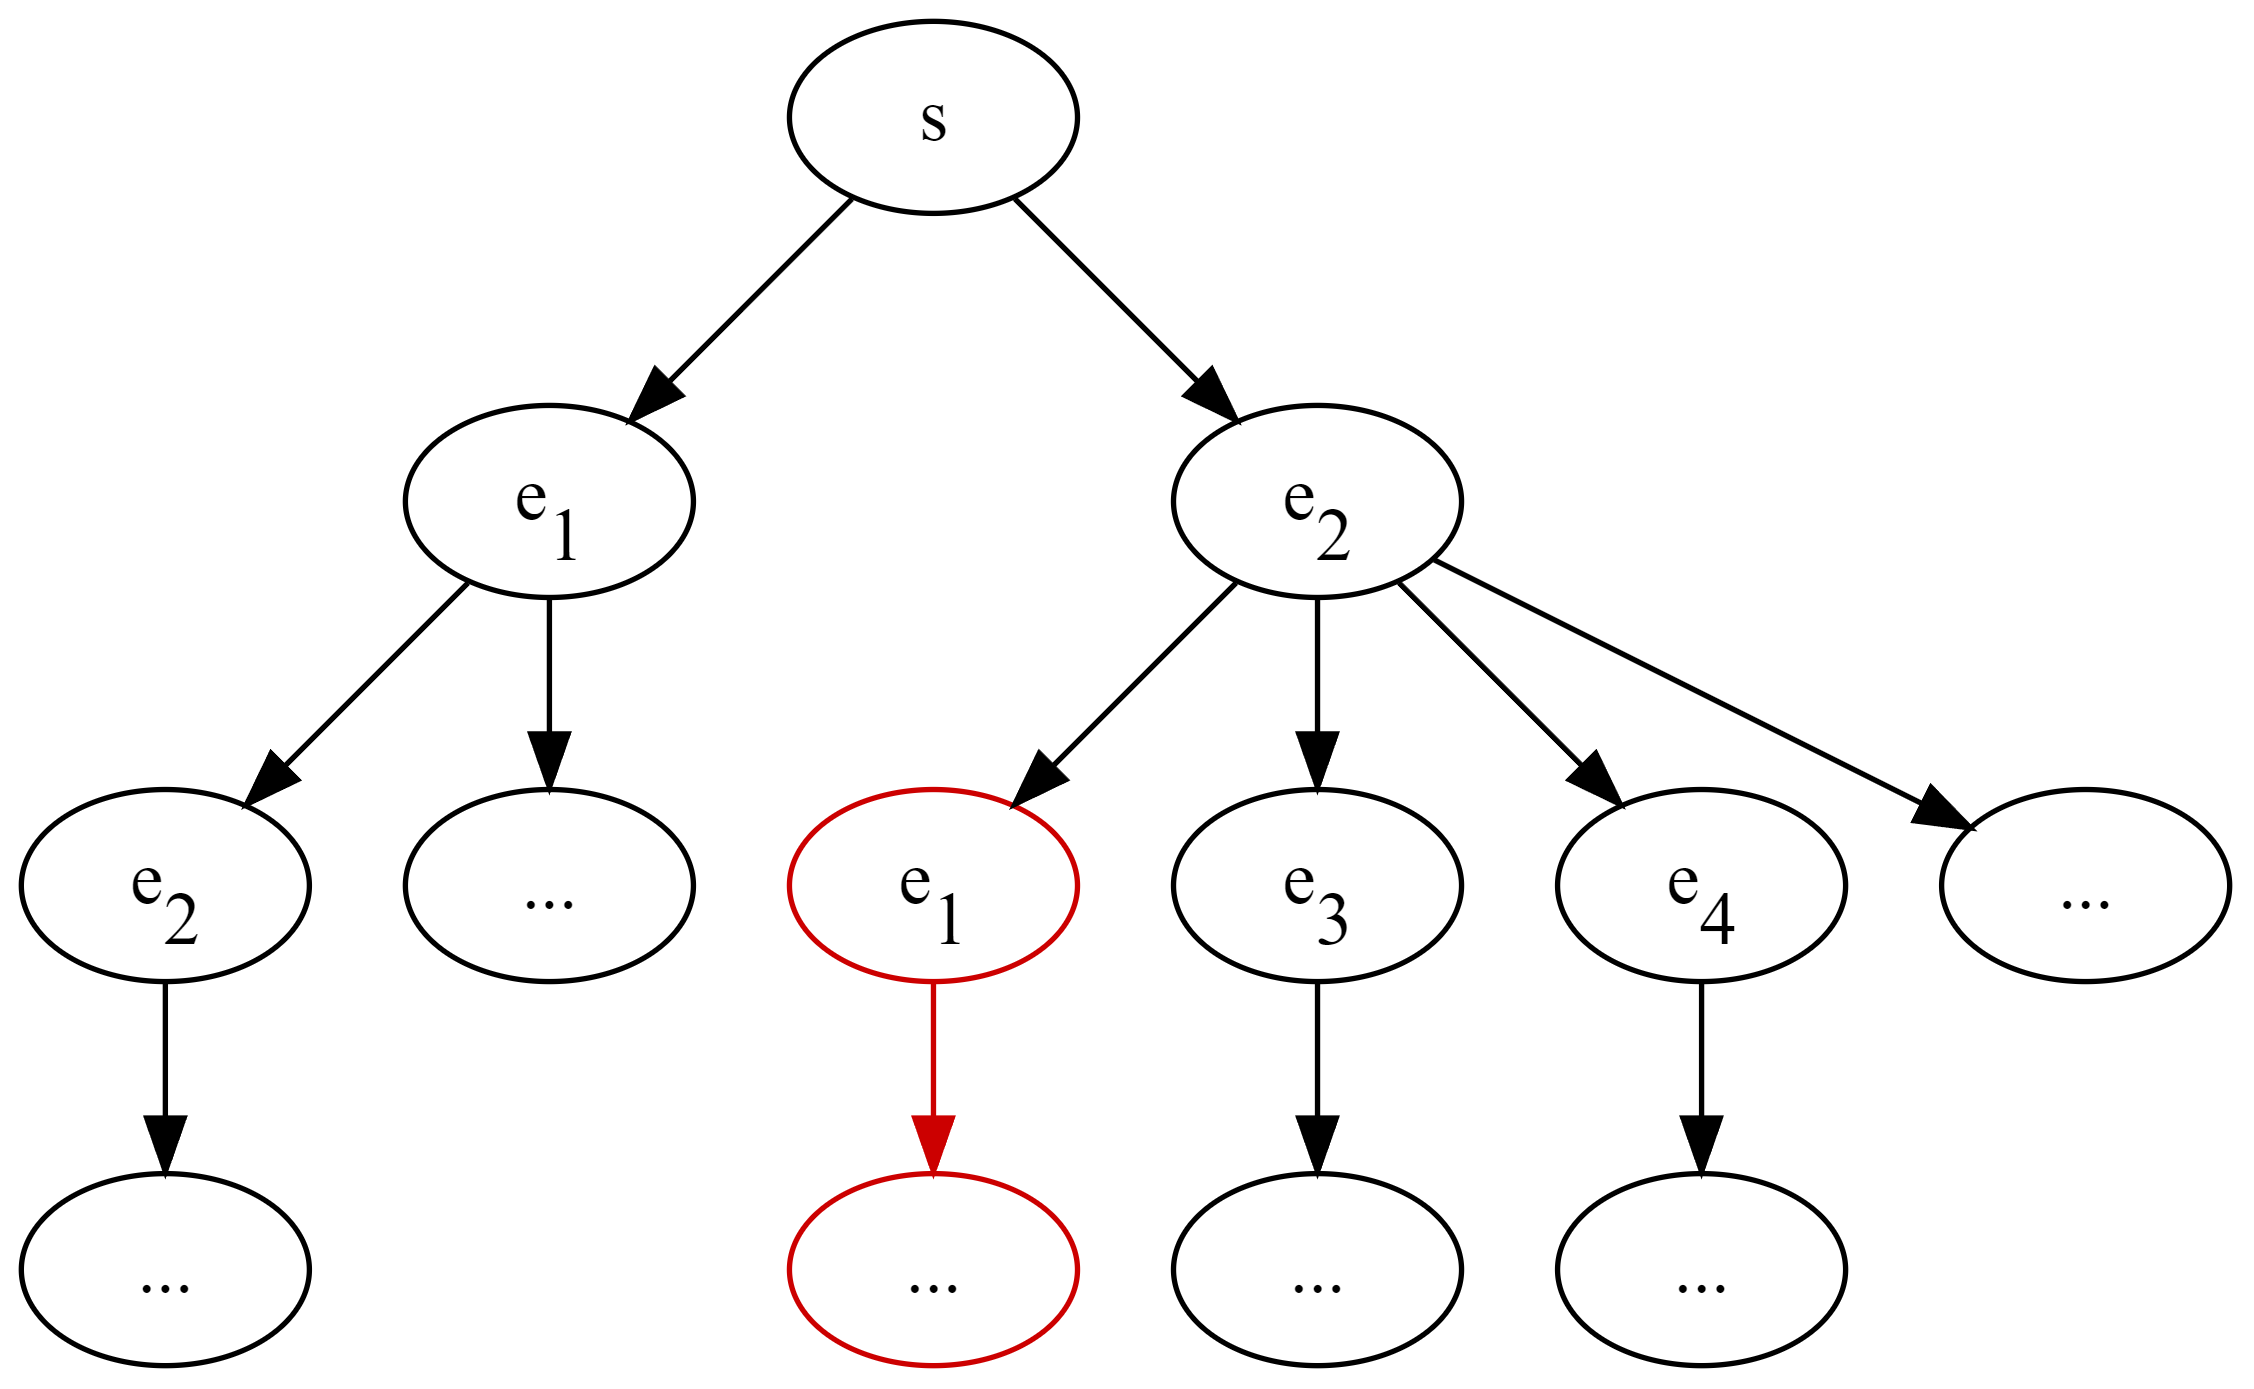
\includegraphics[width=0.85\linewidth]{img/DFS-graph.png}
    \caption{Example search tree for optimal solution completion}
    \label{fig:dfs-graph}
\end{figure}

Regular depth-first search marks each node in a graph as visited once it processes it, meaning that it will not come back to the same node again.
On the other hand, DFS used in the optimal completion cannot skip a potential takeoff just because it already encountered it at some previous time.
Consider a very simple example of a search tree in Figure \ref{fig:dfs-graph}, with a partial solution $s$ in the root node.
Let us start by inserting takeoff $e_1$, followed by takeoff $e_2$, as shown in the left branch.
Other takeoffs may also be inserted and evaluated, but that is irrelevant.
After the search in the left branch is completed and we have the best solution which contains $e_1$, the algorithm moves on to the right branch.
It starts by inserting the takeoff $e_2$, even though it was already visited in the left branch.
This is because the contexts are different -- in the left branch $e_2$ was explored in the context of an already inserted $e_1$, which most likely blocked some other potential takeoffs.
In the right branch, $e_2$ has an empty context because it is being inserted directly into $s$.
The next step would be to insert $e_1$.
However, that is unnecessary because we would get a partial solution $s \cup \{ e_1, e_2 \}$, which is a superset of the partial solution $s \cup \{ e_1 \}$, and that was already fully explored in the left branch.
Therefore, the red nodes in the tree are skipped during the search.

In order to keep track of which nodes can be safely skipped, thus reducing the search space, a set of visited takeoffs $V$ is used.
As mentioned, it does not contain all visited takeoffs, but only those that were already fully explored in the same context.
In practical terms, the visited set contains the left siblings of every ancestor of the currently observed node.
It does not contain the ancestors themselves, although including them would not make a difference. 
The ancestors cannot appear again in the currently explored subtree because they were already inserted into the current partial solution.
As an example, consider the takeoff $e_4$ in Figure~\ref{fig:dfs-graph}.
The visited set for that node would be $V = \{ e_1, e_3 \}$.
At the start of the search, $V$ is an empty set (line~\ref{alg:repair-line-optimal}).

In line~\ref{alg:repair-line-remove-visited} it can be seen that all takeoffs in the visited set $V$ are removed from $C$, the set of potential takeoffs that need to be explored.
Before starting a new recursive call, i.e., descending a level in the search tree, the takeoff $e$ is inserted into a copy of the current partial solution (line~\ref{alg:repair-line-recursion}).
The function result is the best solution in the searched subtree.
The function recursively calls itself for every child node (subtree) in the search tree, and tracks the best found solution.
It should be noted that the search tree is implicit and the set of potential takeoffs changes depending on which takeoffs were previously inserted.


\section{Simulated Annealing}\label{sec:simulated-annealing}

\textit{Simulated annealing} (SA) is an iterative, single-solution based metaheuristic algorithm inspired by the annealing process used in metallurgy, and the Boltzmann's law~\cite{Kirkpatrick/SA}.
This probabilistic technique is based on a Monte Carlo model which simulates energy levels in cooling solids~\cite{Misevicius/SA}.
The main idea behind simulated annealing is the possibility to accept non-improving solutions in order to escape from a local optimum, delaying the convergence and hopefully finding an ever better solution.

The most common method of updating the current solution $s$ is as follows:
if the generated neighboring solution $s'$ is better than the current solution, accept it;
if it is worse, accept it with a probability which depends on the current value of the control parameter $T \ge 0$, and the relative fitness $\Delta f = f(s') - f(s), \, \Delta f \le 0$.
For a maximization problem, the probability of acceptance of a non-improving solution is equal to $P(\Delta f) = e^{\Delta f / \, T}$.
This makes it less likely to accept far worse solutions which have a larger absolute value of $\Delta f$.

The control parameter $T$ represents the temperature in the real-world annealing process.
At high temperatures, the probability of acceptance will be higher, resembling random local search at extreme temperatures.
To facilitate convergence, the temperature is usually gradually reduced, intensifying the search in the process.
At the lowest temperature, $T = 0$, only improving solutions are accepted, resulting in a hill-climbing algorithm.

In the proposed algorithm, a homogeneous cooling schedule is used, slightly decreasing the temperature in every iteration, starting from the initial temperature $T_0$.
A simple geometric decrement function is used: $T \gets \beta \cdot T$.
The cooling factor $\beta \in [0, 1]$ determines the cooling speed, with a usual value very close to $1$.
Another popular decrement function is the \textit{very slow decrease}: $T \gets T \, / \left( 1 + \gamma \cdot T \right), \, \gamma \ge 0$.
However, at the beginning, this function reduces high temperatures far too rapidly, which is not suitable for use with very large absolute values of the objective function and its differences, as is the case in this optimization problem.
In order to have a meaningful probability of acceptance, an average $\Delta f$ and $T$ need to have roughly the same magnitude, making geometric decrease a better choice.

Simulated annealing is a part of local search, so it is integrated into Algorithm~\ref{alg:localsearch}.
At the beginning, the current temperature $T$ is set to the initial temperature $T_0$ (line~\ref{alg:localsearch-line-temp-init}).
In line~\ref{alg:localsearch-line-sa-accept}, the acceptance criteria are checked to see if the current solution should be replaced by the sampled solution.
Finally, the current temperature is updated in line~\ref{alg:localsearch-line-sa-end}, and the next iteration can commence.

State-of-the-art simulated annealing algorithms do not necessarily only decrease the temperature, but rather oscillate it~\cite{Misevicius/SA}\cite{Ma/InhomogeneousSA}.
This leads to reannealing (reheating), which can improve the found solutions.
However, it seems to have almost no effect on this particular problem, and results in approximately doubled execution time for local search.
Therefore, it was not included in the proposed algorithm.


\newcommand{\comment}[1]{}
\comment{

-- fig:dfs-graph --
https://dreampuf.github.io/GraphvizOnline
digraph G {
  e11[label=<e<SUB>1</SUB>>];
  e12[label=<e<SUB>1</SUB>>, color="#cc0000"];
  e21[label=<e<SUB>2</SUB>>];
  e22[label=<e<SUB>2</SUB>>];
  e3[label=<e<SUB>3</SUB>>];
  e4[label=<e<SUB>4</SUB>>];
  s -> e11;
  e11 -> e21 -> dots11;
  e11 -> dots1;
  s -> e22;
  e22 -> e12;
  e12 -> dots22 [color="#cc0000"];
  e22 -> e3 -> dots3;
  e22 -> e4 -> dots4;
  e22 -> dots2;
  dots1[label=<...>];
  dots2[label=<...>];
  dots3[label=<...>];
  dots4[label=<...>];
  dots11[label=<...>];
  dots22[label=<...>, color="#cc0000"];
}

}

\chapter{Implementation}

\section{Technologies}

The heuristic algorithm was implemented in software using the programming language C++, specifically C++20, the standard's latest revision.
Build automation was achieved with CMake, version 3.21.
Source code was compiled with Microsoft Visual C++ (MSVC) compiler.
Even though other compilers were not tested, both GCC and Clang are also supposed to support all of the used language features.
There are no known limitation with respect to the operating system, although the development and benchmarking was performed exclusively on Windows 10.
The application can be compiled both for 32-bit and 64-bit system, without any noticeable performance differences.

Only the central processing unit (CPU) is used for program execution.
The implementation does not rely on the graphics processing unit (GPU) for massive parallelization, in order to have the simplest hardware requirements.
However, it does extensively employ multiple processing units at once in the form of multithreading.

There are no special requirements in the developed program that would warrant the use of any specialized programming language.
C++ was chosen over other programming languages simply because of the performance benefits.
With the time limit set aggressively low at ten minutes, it was necessary to maximize the hardware's potential, which was done in part by the choice of a programming language.


\section{Input Data Formats}

All input parameters are passed to the program in the form of an input file or read from the standard input stream (stdin).
Two textual representations are supported, referred to as \textit{AMPL format} and \textit{simple format}.


\subsection{AMPL Format}

A problem-specific subset of the AMPL data format is supported.
AMPL is an algebraic modeling language used for mathematical computing.
The full format specification is described in detail in Ref~\cite{Fourer/AMPL}.
This section focuses on the few features supported in the developed program, and explains requirements which have to be met in order for the input data to be correctly interpreted by the program.
This format is primarily supported for compatibility reasons, so that the same input data files can be read as the ones used in Ref~\cite{SkorinKapov/ILP}, simplifying the algorithm comparison.

An example of data in this format is shown in Appendix~\ref{appx:input-file-ampl}.
Real input data must closely follow this example.
The names of sets and parameters are irrelevant, as long as their order is the same.
The names of elements in sets of aircraft, fire fronts, and aircraft types must be a single letter followed by an integer.
These elements must always appear in ascending order, including when used as labels for rows or columns of matrices.
Time slots must also always be used in ascending order.
The numbering of all elements and labels must be one-based.
The number and positioning of blank lines between different parameters, as well as within matrix definitions, must be strictly respected. 
Comments (starting with \texttt{\#}) may only appear in the same places as in the example, but can also be omitted as long as the preceding semicolon stays in the same line.
The number of separating spaces and tabulators between labels and values in the same line is irrelevant, as long as there is at least one separating character.

In the set of aircraft types, \texttt{Q1} and \texttt{Q2} represent helicopters and airplanes, respectively.
Only these two types are allowed, and both must be present.
The second row of matrix \texttt{V} is ignored.
Strictly speaking, it should be a negation of the first row, which contains values for the parameter $V_k$.
The second row of matrix \texttt{B} is also ignored, and should always contain only zeroes, as it is not allowed to restrict a fire front only to airplanes.
The first row contains values for the parameter $B_f$.
The parameter \texttt{M} is a large integer constant used in the ILP formulation, and ignored in the input data.
The usage of all other parameters is self-explanatory, and backed by comments in the example data.

It should have been possible to use the AMPL C++ API, which exists for Windows, Linux and macOS, in order to parse the input data file.
That would have removed all of the aforementioned restrictions, on top of eliminating the need for a custom data parser.
However, it was decided against using the API to avoid licensing issues, as well as having a library dependency which is platform dependent.


\subsection{Simple Format}

Unless AMPL API is used, generating and parsing AMPL data files is unnecessarily complicated.
To help alleviate this issue, another input data format was designed, aptly named the \textit{simple format}.
An example of data in this format is given in Appendix~\ref{appx:input-file-simple}.
Data in this example is the same as in Appendix~\ref{appx:input-file-ampl}.

Data consists only of integers and floating point numbers, separated by one or more whitespace characters.
Different whitespace characters can be freely mixed.
The most compact representation would be a single line of text with the numbers separated by a single space character.

Parameters have a predefined order.
For parameters which are matrices, \textit{row-major} order is used, meaning the leftmost index changes the least frequently.
The order of aircraft and fire fronts is irrelevant, as long as it is the same throughout the input data.
The time slots must be sorted and indexed such that the earliest time slots is the first one.
The order is as follows:
\begin{itemize}
    \item the number of aerial resources $\vert \mathcal{K} \vert$,
    \item the number of fire fronts $\vert \mathcal{F} \vert$,
    \item the number of time slots $\vert \mathcal{T} \vert$,
    \item vectors $V_k$, $T_k$, $R_k$, $P_k$, $N_k$,
    \item matrix $A^t_k$, indexed as $A[t][k]$,
    \item vector $B_f$,
    \item matrix $U_{kf}$, indexed as $U[k][f]$,
    \item vectors $C_k$, $S_f$,
    \item matrix $D^t_{kf}$, indexed as $D[f][t][k]$,
    \item matrix $E^t_{kf}$, indexed as $E[f][t][k]$,
    \item matrix $W^t_f$, indexed as $W[t][f]$,
    \item $a_1, a_2, a_3$.
\end{itemize}

Note that, for the most part, the simple format is just the AMPL format with all labels removed, keeping only the important numerical values in the same predefined arrangement.
Compared to the AMPL format, this format eliminates declaring the aircraft and fire front sets, simplifies defining the type of each aircraft and type limitations for fronts, and removes the redundant ILP parameter $M$.

If the data generation is done in software, for example, as an export from a graphical user interface, it should be considerably easier to generate input data in this format compared to the AMPL data format.
The only noticed downside is limited readability for humans because of the lack of annotations, especially if newline characters are not consistently used to separate different parameters into groups.


\section{Output Data}

\begin{table}[htbp]
\caption{Keys and descriptions of some output values}
\label{tbl:output-params}
\small
\centering

\newcommand{\twoline}[2]{\begin{tabular}[t]{@{}l@{}}\texttt{#1} \\ \texttt{#2}\end{tabular}}
\newcommand{\threeline}[3]{\begin{tabular}[t]{@{}l@{}}\texttt{#1} \\ \texttt{#2} \\ \texttt{#3}\end{tabular}}
\newcommand{\thinline}{\specialrule{.001em}{.2em}{.2em}}

\begin{tabularx}{\hsize}{@{}lX@{}}
Key & Description \\
\midrule
\texttt{WO}        & The total water output (positive). \\
\texttt{Sum\_WSn}  & The total negative water surplus (negative or zero). \\
\texttt{Z}         & The minimal water surplus (any real value). \\
\texttt{objective} & The objective function value (any real value). \\

\thinline

\texttt{\_solve\_wall\_time}    & The duration of the entire execution. \\
\texttt{\_takeoffs\_count}      & The number of takeoffs in the best schedule. \\
\texttt{\_takeoffs\_count\_max} & The theoretical upper limit on the number of takeoffs for the given input parameters. \\
\texttt{\_best\_iteration}      & The ordinal number of the GRASP iteration which yielded the best schedule, using one-based indexing. \\
\texttt{\_total\_iterations}    & The total number of executed GRASP iterations. \\
\texttt{\_threads}              & The number of worker threads in the thread pool. \\

\thinline

\threeline{\_objective\_greedy\_best}{\_objective\_greedy\_avg}{\_objective\_greedy\_stddev} & The best value, arithmetic mean, and standard deviation of the objective function values of all solutions constructed in the greedy phase of GRASP. \\
\thinline
\twoline{\_objective\_ls\_avg}{\_objective\_ls\_stddev}             & Arithmetic mean and standard deviation of the objective function values of all solutions found by local search. \\
\thinline
\twoline{\_duration\_iteration\_avg}{\_duration\_iteration\_stddev} & Arithmetic mean and standard deviation of the duration of all GRASP iterations. \\
\thinline
\twoline{\_duration\_greedy\_avg}{\_duration\_greedy\_stddev}       & Arithmetic mean and standard deviation of the duration of the greedy phase of GRASP. \\
\thinline
\twoline{\_duration\_ls\_avg}{\_duration\_ls\_stddev}               & Arithmetic mean and standard deviation of the duration of local search. \\

\thinline

\texttt{\_durations\_iteration} & A list durations for every GRASP iteration. \\
\texttt{\_durations\_greedy}    & A list durations for every greedy construction phase. \\
\texttt{\_durations\_LS}        & A list durations for every local search. \\
\end{tabularx}
\end{table}

The program output contains relevant information on the best found schedule in a human-readable format.
An example of such output is given in Appendix~\ref{appx:output-file}.
The output is always sent to the standard output stream (stdout), and also to an output file if explicitly requested.

In the beginning, the output data gives an overview of the three objective values, followed by values related to the performance of the algorithm.
Results of both phases of every GRASP iteration are aggregated, and the arithmetic means and standard deviations of the objective function values and execution times are given.
Table~\ref{tbl:output-params} lists and describes all of the simple output values.
All durations are measured as elapsed real time, in seconds.

The bulk of the output data is related to different representation of the best schedule.
The order of all rows, columns, indices, etc., is the same as the order in the input data.
All indexing is zero-based.

The first representation, called \textit{condensed schedule}, is the most compact.
It is a two-dimensional $\vert \mathcal{K} \vert \times \vert \mathcal{T} \vert$ matrix, with elements representing the number of the front on which the aircraft is flying in the relevant time slot.
A dash symbol means the aircraft is not flying, either because it is resting or is unavailable.

The full schedule is a three-dimensional $\vert \mathcal{K} \vert \times \vert \mathcal{F} \vert \times \vert \mathcal{T} \vert$ boolean matrix.
It is an expanded version of the condensed schedule.
Each block of values represents one aircraft, labeled with \texttt{x = k} for easier navigation.
Elements take value $1$ if the corresponding aircraft is flying at the fire front during the time slot.
Value $0$ means the aircraft is not flying at that specific front, but it might be flying elsewhere.

The takeoffs matrix is the same as the model's decision variable, with boolean elements $c_{kf}^t$.

Finally, a two-dimensional $\vert \mathcal{F} \vert \times \vert \mathcal{T} \vert$ matrix of water surplus per fire front and time slot is given, with elements $\mathit{WS}_{tf} \in \mathbb{R}$.
Using this information, the input parameters can be tuned and the algorithm can be executed again if needed.
For example, the target water content can be increased on some fronts, or an aircraft can be sent to a faraway base because it is actually not needed.


\section{Command-line Flags}

All program's parameters are set via command-line flags, including every hyperparameter used in pseudocode.
Every flag has a reasonable default value in order to simplify launching the program.
Flags are handled by a command line parser library licensed under the 3-clause BSD license~\cite{Schreiner/CLI11}.

The most important flags are \texttt{-i,-{}-input} and \texttt{-o,-{}-output}.
They are used to set the paths to the input and output files.
If the values are "\texttt{-}" (default), the standard input and output streams are used instead.
Considering that two different input file formats are supported, the flag \texttt{-f,-{}-format} is used to set the exact input format.
While it would have been possible to assume AMPL data format was used if data started with \texttt{data;}, that was not done in case a third format has to be introduced in the future.

The flag \texttt{-t,-{}-threads} can be used to set the number of worker threads.
For maximum performance, the value should be between the number of physical CPU cores and the number of logical processors.
Setting a value higher than the number of logical processors will most likely result in slower execution than if a lower number was selected.

A comprehensive list of flags, their arguments' types and default values, as well as their descriptions, are depicted in Table~\ref{tbl:cli}.
If the program is executed with the \texttt{-h,-{}-help} flag, a help message with similar information is printed and the program is terminated.

The following is an example of how one might start the program: \newline
\texttt{AerialResourceScheduler.exe -i~input.dat -o~results.txt \\ -f~ampl -t~8 -{}-iters~40}

\begin{table}[htbp]
\caption{Supported command-line flags}
\label{tbl:cli}
\fontsize{10.6pt}{13.3pt}\selectfont
\centering
\begin{tabularx}{\hsize}{@{}llllX@{}}
Flag & Type & Default & Parameter & Description \\
\midrule
\texttt{-i,-{}-input}   & string & \texttt{-}     & \texttt{N/A}       & Path to input file. Reads from stdin if omitted or set to a dash symbol. \\
\texttt{-o,-{}-output}  & string & \texttt{-}     & \texttt{N/A}       & Path to output file. Skips printing to a file if omitted or set to a dash symbol. \\
\texttt{-f,-{}-format}  & enum   & \texttt{ampl}  & \texttt{N/A}       & Input data format. Either \texttt{ampl} or \texttt{simple}. \\
\texttt{-t,-{}-threads} & uint   & \texttt{1}     & \texttt{N/A}       & Number of worker threads. \\
\texttt{-{}-iters}      & uint   & \texttt{20}    & $\mathit{iterations}$ & Total number of GRASP iterations to run. Preferably a multiple of \texttt{-{}-threads} for maximum efficiency. \\
\texttt{-{}-ls-iters}   & uint   & \texttt{6000}  & $L$                   & Number of iterations in local search. \\
\texttt{-{}-nd}         & uint   & \texttt{5}     & $N_D$                 & Number of takeoffs to be removed in destroy method. \\
\texttt{-{}-nr}         & uint   & \texttt{3}     & $N_R$                 & Number of takeoffs to be added in greedy part of repair method. \\
\texttt{-{}-alpha-g}    & float  & \texttt{0.10}  & $\alpha_G$            & Alpha value for RCL in greedy construction. \\
\texttt{-{}-alpha-d}    & float  & \texttt{0.75}  & $\alpha_D$            & Alpha value for RCL in destroy method. \\
\texttt{-{}-alpha-r}    & float  & \texttt{0.10}  & $\alpha_R$            & Alpha value for RCL in greedy part of repair method. \\
\texttt{-{}-kr-g}       & float  & \texttt{4.0}   & $k_{r, G}$            & Kr weight in greedy construction. \\
\texttt{-{}-kp-g}       & float  & \texttt{4.0}   & $k_{p, G}$            & Kp weight in greedy construction. \\
\texttt{-{}-kr-r}       & float  & \texttt{1.0}   & $k_{r, R}$            & Kr weight in greedy part of repair method. \\
\texttt{-{}-kp-r}       & float  & \texttt{1.0}   & $k_{p, R}$            & Kp weight in greedy part of repair method. \\
\texttt{-{}-t0}         & float  & \texttt{1e12}  & $T_0$                 & Starting temperature T0 in SA. \\
\texttt{-{}-temp-coeff} & float  & \texttt{0.995} & $\beta$               & Cooling factor in SA. \\
\end{tabularx}
\end{table}


\section{Schedule Class}

Takeoffs are modeled as a simple data structure (\texttt{struct}) consisting of three unsigned bytes (\texttt{std::uint8\_t}) representing the ordinal numbers of the aircraft, the fire front, and the time slot.
This way, $2^8 = 256$ different aerial resources, fire fronts, and time slots can be defined in the input data, far exceeding any real world requirements, while at the same time slightly reducing the amount of used memory.
Of course, the ordinal numbers themselves are pointless outside of the context of a problem instance, which contains all the information parsed from the input data.

A schedule is modeled as a relatively complex class.
Much like in the pseudocode, the main part of a schedule is a set of takeoffs which constitute it.
For typical problem instances, the takeoff matrix is rather sparse (usually between $1\%$ and $4\%$ of elements have their value set to $1$), so using a set to represent a sparse matrix makes sense.

In order to improve performance, various calculations and constraint violations are cached, for example, the number of remaining available takeoffs for each aircraft, the number of remaining places in the carousel per front and time slot, the water surplus per front and time slot, as well as the total water output.
Overall, great care was taken to reduce the execution time as much as possible.
Throughout development even minor changes to the implementation were benchmarked to determine the most performant choice.

The schedule keeps track of the number of constraints that are violated for every possible takeoff -- all $\vert \mathcal{K} \vert \cdot \vert \mathcal{F} \vert \cdot \vert \mathcal{T} \vert$ of them.
It is implemented as a three-dimensional matrix of unsigned bytes, in order to keep the memory usage low.
At the beginning, it is initialized to block takeoffs which would be in conflict with aircraft availability, or begin too late for the aircraft to return to base in time, or would have an aircraft of the wrong type flying on a type-restricted fire front.
Each inserted (removed) takeoff increases (decreases) the constraint violation counters.
A value of $n$ could mean that a single constraint would be violated for $n$ takeoffs, or $n$ constraints would be violated for a single takeoff, or anything in between.
If a value in the matrix is greater than zero, it means that the corresponding takeoff cannot be inserted in the current schedule because it would break one or more constraints, for example, because the same aircraft is already flying during that time slot, or because pilot's physical presence limit would be exceeded, or an aircraft of a different type is already scheduled to be flying at that front at any point during the prospective flight, etc.
However, if the value in the matrix is equal to zero, it still does not mean it is legal to insert the takeoff, because not every constraint is tracked in this manner.
The two constraints tracked separately are the number of remaining available takeoffs per aircraft, and the number of remaining places in the carousel per fire front and time slot.
Only if all of the constraints are satisfied can the takeoff be considered feasible.

Contrary to what is depicted in the pseudocode, making copies of a schedule was avoided whenever possible.
The only exceptions are when the incumbent solution needs to be updated, so a copy of the schedule is stored as the best found solution so far.
In all other situations, manipulations on the schedule are done in-place, by inserting and removing takeoffs.
For example, values of functions $o(e)$ and $p(e)$ defined in lines \ref{alg:greedy-line-o-def} and \ref{alg:greedy-line-p-def} of Algorithm~\ref{alg:greedy} are calculated by inserting the takeoff $e$, computing the needed values, and then removing the takeoff $e$ from the schedule.
Compared to making a copy of the schedule, inserting a takeoff, and then discarding it, this approach lowered execution time approximately five times.


\section{Algorithm Parallelization}

Looking at the loop in line~\ref{alg:grasp-line-for-loop} of Algorithm~\ref{alg:grasp}, it can be seen that each iteration is almost completely independent from all others.
Iterations are only coupled by the aggregation phase of the algorithm, where the best solution from all iterations is chosen.
This makes the whole search algorithm trivially parallelizable, since GRASP is the top-level metaheuristic.

Parallelization is performed via a thread pool, where each GRASP iteration is a task that needs to be solved, sent into the task queue.
A thread pool library is used, licensed under the MIT License~\cite{Shoshany/ThreadPool}.
The worker threads repeatedly take tasks out of the queue, execute the search, and return the found solution.
The main thread iterates over all submitted tasks, outputting the value of the objective function for the found solution as each iteration finishes, as well as updating the incumbent solution.
This way, the user has a live insight into the progress of the search, as opposed to waiting until all iterations finish.
Once all the tasks are finished, detailed information about the best found solution is output to the standard output stream, and possibly a file if specified.
This marks the end of the program, and the process is terminated.

During development, a peculiar issue was discovered after GRASP was parallelized.
Even though different threads did not appear to share any resources, using 12 worker threads on a CPU with 12 physical cores resulted in roughly three times performance improvement, instead of the expected 12 times, compared to the single-threaded performance.
However, when multiple single-threaded processes were started, the performance improved linearly.
For example, executing 12 processes at once did in fact take the same amount of time as executing a single process.
This means that the memory bandwidth and the amount of available CPU cache are not the limiting factors.

The main cause of the slowdown were allocations of a larger amount of contiguous memory than necessary, in a function which looks for and returns all feasible takeoffs.
To be exact, almost 150~KiB were reserved for each returned \texttt{std::vector} (one per function call), while most often just a few hundred bytes were actually being used.
This memory was released shortly after it was reserved, and no more than five of those vectors were allocated at the same time.
Per GRASP iteration, this was done almost $2.5$~million times, resulting in a total of over 350~GiB of memory being reserved each iteration.
When 12 iterations were being executed at the same time, in total over 4~TiB of memory was reserved and released in the span of approximately 20 seconds.
Granted, the actual RAM usage was rather low, and stayed under 10~MiB throughout the entire execution.
The issue was remedied by not proactively reserving any memory, and letting the vector increase its size as needed.
The most interesting observation was that the amount of reserved memory had almost no impact on single-threaded performance.
If fact, the performance slightly improved when memory was allocated ahead of time, but not to the point where it would be immediately noticeable.

It is suspected the issue was related to heap contention.
In the case of multiple single-threaded processes, each of them has its own heap.
In a multithreaded process, each thread has a separate call stack, but there is only one shared global heap.
For multiple threads to be able to simultaneously allocate and deallocate memory, the heap must be thread-safe.
Access to the heap is automatically serialized, meaning that while one thread's request is not finished, the other threads will be blocked.
This is the default behaviour, which can be changed if a custom memory allocator is used~\cite{Ferreira/MemoryAllocators}.
An \texttt{std::vector} stores data on the heap, so that it can be automatically resized as needed.
Allocating so many vectors from a dozen threads at once most likely resulted in memory contention.


\section{Algorithm Time Complexity}

\def\Tkmax{T_{k, \mathrm{max}}}

To simplify notation, aliases for the sizes of sets are defined: $K = \vert \mathcal{K} \vert,\, F = \vert \mathcal{F} \vert,\, T = \vert \mathcal{T} \vert$.
Auxiliary variables are used to denote the maximum number of takeoffs in a valid schedule ($S$), and the longest flight time ($\Tkmax$):
\begin{equation}
S = \sum_{k \in \mathcal{K}}{N_k}
\end{equation}
\begin{equation}
\Tkmax = \max_{k \in \mathcal{K}} T_k
\end{equation}

Time complexity of the randomized greedy algorithm is given in Equation~\ref{eq:big-o-greedy}.
It is dominated by searching for all feasible takeoffs that could be inserted in the next iteration of the construction phase, i.e., evaluating the function $p(e)$ (Algorithm~\ref{alg:greedy}, line~\ref{alg:greedy-line-p-def}).
\begin{equation}\label{eq:big-o-greedy}
\mathcal{O} \left(
S \cdot \Tkmax \cdot \left( K F T \right) ^ 2
\right)
\end{equation}
Algorithm complexity of each local search iteration is given in Equation~\ref{eq:big-o-ls-long}.
The last term is related to depth-first search.
However, in practice, the base (representing feasible takeoffs) is significantly smaller than $K F T$ and $N_D - N_R \le 2$ is often used, meaning that the complexity can be approximated by Equation~\ref{eq:big-o-ls-short}.
\begin{equation}\label{eq:big-o-ls-long}
\mathcal{O} \left(
N_R \cdot \Tkmax \cdot \left( K F T \right) ^ 2 + \left( K F T \right) ^ {N_D - N_R}
\right)
\end{equation}
\begin{equation}\label{eq:big-o-ls-short}
\mathcal{O} \left(
N_R \cdot \Tkmax \cdot \left( K F T \right) ^ 2
\right)
\end{equation}
If $\Tkmax$ and $N_R$ are assumed to be constants, and $\mathcal{O}(S) = \mathcal{O}(K)$ is assumed, the complexities can be simplified even further.
Finally, by combining the complexities for each GRASP phase and applying the simplifications, the algorithm complexity for a single GRASP iteration can be found:
\begin{equation}\label{eq:big-o-grasp}
\mathcal{O} \left(
\left( L + K \right) \cdot \left( K F T \right) ^ 2
\right)
\end{equation}
Equation~\ref{eq:big-o-grasp} shows that the implemented heuristic algorithm has polynomial time complexity.

\chapter{Test Scenarios}\label{chap:test-scenarios}

Because the model described in this thesis was designed in Ref~\cite{SkorinKapov/ILP}, and at the time of writing no other research was done relating to that specific model, there are no standard benchmark datasets available other than those used in Ref~\cite{SkorinKapov/ILP}.
They were programmatically generated, and the same generator, albeit with different parameters, was used in this thesis.
The test scenarios are generated in a way that respects Spanish regulations~\cite{Spain/AnnexCircular}.
Parameter values have similarities with those of real aerial resources and real situations, but do not portray any specific wildfire.


\section{General Parameter Values}

It is assumed that daylight hours are between 7:00 and 22:00, which is representative of a typical summer day in Spain.
This results in 15 hours of daytime, split into 45 time slots, each 20 minutes long: $\mathcal{T} = \left\{ 1, \ldots, 45 \right\}$.

Test scenarios come in seven different sizes with respect to the number of aerial resources and fire fronts.
Helicopters make up around $65\%$ of all aerial resources, and airplanes account for the remaining $35\%$.
Helicopters are further divided into light, medium, heavy and military categories, with approximately $50\%$, $20\%$, $20\%$, and $10\%$ shares, respectively.
The exact numbers are depicted in Table~\ref{tbl:scenario-sizes}.

\begin{table}[htb]
\caption{Sizes of test scenarios and the number of aircraft per subtype}
\label{tbl:scenario-sizes}
\centering
\footnotesize
\begin{tabular}{lrr|*5r}
Scenario & Aircraft & Fronts & Light h. & Medium h. & Heavy h. & Military h. & Airplanes \\
\midrule
K07\_F02 & 7  & 2 & 2  & 1 & 1 & 0 & 3  \\
K10\_F03 & 10 & 3 & 3  & 1 & 1 & 1 & 4  \\
K15\_F03 & 15 & 3 & 5  & 2 & 2 & 0 & 6  \\
K20\_F04 & 20 & 4 & 7  & 3 & 3 & 0 & 7  \\
K25\_F04 & 25 & 4 & 8  & 3 & 3 & 2 & 9  \\
K30\_F05 & 30 & 5 & 10 & 4 & 4 & 1 & 11 \\
K35\_F05 & 35 & 5 & 11 & 4 & 4 & 3 & 13 \\
\end{tabular}
\end{table}

Fronts on which airplanes cannot operate are considered to be uncommon -- parameter $B_f$.
There is a $20\%$ chance a test scenario is selected to contain such a front.
If it is selected, a single random front is picked as the one on which only helicopters can operate, while others remain open for airplanes.

The maximum number of aircraft in a carousel, $S_f$, is chosen at random for each fire front, with values in range $[7, 10]$.
The size of an instance has no effect on the size of the carousel as that is determined by the terrain features, such as the number of water points and the size of the fire front.
The carousel size has to be limited so that airspace does not become congested, which increases the risk of a collision.

The Spanish regulations impose a limit on maximum continuous flight time -- parameter $T_k$.
For helicopters that limit is two hours, and for airplanes it is four hours~\cite{Spain/AnnexCircular}.
Legislation also imposes the minimum duration of resting periods between continuous flights -- parameter $R_k$.
In case of helicopters the breaks must be at least 40 minutes, and for airplanes it is at least 80 minutes.
Furthermore, helicopters can make at most four flights in a single day, while airplanes have a lower limit of just two flights per day -- parameter $N_k$.
Regulations limit pilot presence to 12 continuous hours, regardless of aircraft type -- parameter $P_k$.

With respect to availability, $A_k^t$, helicopters are assumed available in all time slots, as they tend to remain in proximity to the fire, and usually do not come from faraway bases.
For airplanes, it is considered that at the start of the day they might have to fly in from a further base where they were previously located, or return to it at the end of the day, perhaps to fight another wildfire the following day.
An example of the distribution of airplanes across different bases is shown in Figure~\ref{fig:spain-airplanes-deployment}.
The availability is as follows:
\begin{itemize}
    \item $85\%$ chance the airplane is available throughout the entire day,
    \item $10\%$ chance it is unavailable at the beginning of the day, with unavailability ending between 10:20 and 13:00,
    \item $5\%$ chance it is unavailable at the end of the day, with unavailability starting between 18:20 and 20:00.
\end{itemize}
In case an airplane was unavailable for a part of the day, one flight is deducted from the available daily quota, with the reason being that it was spent on transit between bases of operation.
Consequently, one airplane cannot be unavailable both in the morning and in the evening, as deducting two flights would leave it without any flights to spend fighting the fire.

All helicopters are assumed to be able to reach any front within a single time slot -- parameter $U_{kf}$ is given value $0$.
This is because helicopters are more flexible with respect to takeoff and landing and can thus depart from and return to a larger set of destinations (airports, bases, fields, or even parking lots) which are typically within 20~minutes of the fire~\cite{INFOCACongreso2017}.
On the other hand, airplanes require a runway, so the choice of bases is limited.
Furthermore, longer transit times are less of an issue for airplanes because of their longer maximum flight duration.
For those reasons, the value of parameter $U_{kf}$ is randomly set to $0$, $1$, or $2$ for every airplane.
Whichever value is selected, it is the same for all fronts.

\begin{table}[htb]
\caption{Water capacities and average drops per hour for each aircraft subtype}
\label{tbl:capacity-and-droprate}
\centering
\small
\begin{tabular}{lrrl}
Aircraft subtype    & Capacity ($C_k$) & Avg. drops & Aircraft models \\
\midrule
Light helicopter    & \SI{900}{\liter}  & $5$ & AS350B3, A119 Koala \\
Medium helicopter   & \SI{1500}{\liter} & $5$ & Bell 412, W-3 Sokół \\
Heavy helicopter    & \SI{4500}{\liter} & $4$ & Kamov Ka-32 \\
Military helicopter & \SI{2100}{\liter} & $5$ & AS332 Super Puma, NH90 \\
Airplane            & \SI{5500}{\liter} & $3$ & CL-215, CL-415 \\
\end{tabular}
\end{table}

The water capacity and average drops per time slot for each model aircraft are derived from their real-life counterparts~\cite{Frias/Capacities, Sanz/Helicopters, Merida/Evaluation}, and according to data provided by the 43rd Group of the Spanish Air Force.
Values are shown in Table \ref{tbl:capacity-and-droprate}.
The exact number of drops per time slot depends on the features of the front and the time of day.
On some fire fronts the water points could be farther away from the actual fire which in turn lowers the effectiveness and the number of drops that can be made in the same amount of time~\cite{Merida/Evaluation}.
Different weather conditions throughout the day, such as increased wind speed, could also reduce the effectiveness of aerial resources.
For testing purposes, each fire front is given a random accessibility rating between $0.8$ and $1.2$ which is used as a weighting factor for the average drops per time slot (Table \ref{tbl:capacity-and-droprate}), resulting in the drops per firefighting time slot -- parameter $D_{kf}^t$.
Between 15:00 and 18:00 the drops are reduced by $5\%$ to simulate worse weather conditions.
As for hybrid time slots, $E_{kf}^t$, drops per time slot are selected to be equal to between $0\%$ and $50\%$ of their firefighting counterpart, with up to $5\%$ variation between fronts.
That is to simulate the fact that aircraft spend some of the time in transit, as opposed to exclusively fighting the fire.


\section{Distribution of the Target Water Content}\label{sec:water-distribution}

\textit{Total water capacity} (TWC) is estimated by multiplying the maximum number of firefighting time slots for all flights, with the amount of water dropped in an average firefighting time slot, summed across all aircraft.
While the total water output $\mathit{WO}$ will approach TWC when resources are scheduled according to their strengths, the distribution of water output over time and fronts is highly unlikely to be uniform, or otherwise desirable.
In order to set accomplishable goals with respect to the target water content, a different metric has to be used.

\textit{Corrected total water capacity} (CTWC) is calculated by multiplying TWC with the \textit{correction factor} $\mathit{CF}$ -- a value between $0\%$ and $100\%$.
CTWC is used as a guideline on what the sum of the target water content should be for the generated instance -- parameter $W_f^t$.
Two types of categories are used to determine the distribution of water content -- \textit{distribution over time} (DOT) and \textit{distribution over fronts} (DOF).
Distribution over time can be either \textit{initial attack} (IA) or \textit{mostly uniform over time} (MUOT).
Distribution over fronts can be either \textit{uniform over fronts} (UOF) or \textit{non-uniform over fronts} (NUOF).
Categories are combined, giving a total of four possible distributions.

UOF splits CTWC equally over all fronts, whereas NUOF splits it unevenly.
For example, in case of two fire fronts NUOF will delegate $65\%$ of CTWC to the first front, and $35\%$ to the second.
It is used to simulate the fact that some fronts are often more important than others.
That could be the case for a number of reasons, such as the sheer size of the wildfire on that front, requiring more resources to contain it, or perhaps the fact that some front is closer to an inhabited area and needs to be prioritized.

Selected DOT further distributes the delegated water content across time slots.
IA will uniformly distribute $60\%$ of the water over time slots in the first six hours of the day, and the remaining water across the remaining time slots.
MUOT will either distribute the water completely uniformly, or will assign about $15\%$ more water to the time slots between 13:00 and 18:20, for example to simulate stronger winds which increase the risk of the fire spreading.

The first and last time slots of the day are always assigned $75\%$ lower targets.
This is because all aircraft have to either start or end those time slot in their base, i.e., no flight can be in a dedicated firefighting state at those moments.
Because of the nature of the problem, aircraft have very limited suppression capabilities in those time slots.
Setting high targets in the first and last slots would require many resources to be deployed both early and late in the day in order to meet those targets, leaving fewer available flights throughout the bulk of the day, and severely hindering the total suppression efforts.
Reducing those targets allows us to meet them more easily, and $75\%$ empirically showed to be a good reduction factor.


\section{Weighting Factors}

\begin{table}[htb]
\caption{Effects of $a_2$ on negative water surplus}
\label{tbl:weighting-comparison}
\centering
\begin{tabular}{@{}*8r@{}}
~ & ~ & \multicolumn{2}{c}{2 slots} & \multicolumn{2}{c}{3 slots} & \multicolumn{2}{c}{10 slots} \\
\cmidrule(lr){3-4} \cmidrule(lr){5-6} \cmidrule(lr){7-8}
$a_2$ & Objective & Per slot & Total & Per slot & Total & Per slot & Total \\
\midrule
$0.01$  & $-1.01$  & $-0.502$ & $-1.005$ & $-0.336$ & $-1.007$ & $-0.101$ & $-1.009$ \\
$0.10$  & $-1.10$  & $-0.524$ & $-1.048$ & $-0.355$ & $-1.065$ & $-0.109$ & $-1.089$ \\
$0.50$  & $-1.50$  & $-0.600$ & $-1.200$ & $-0.429$ & $-1.286$ & $-0.143$ & $-1.429$ \\
$1.00$  & $-2.00$  & $-0.667$ & $-1.333$ & $-0.500$ & $-1.500$ & $-0.182$ & $-1.818$ \\
$2.00$  & $-3.00$  & $-0.750$ & $-1.500$ & $-0.600$ & $-1.800$ & $-0.250$ & $-2.500$ \\
$10.00$ & $-11.00$ & $-0.917$ & $-1.833$ & $-0.846$ & $-2.538$ & $-0.550$ & $-5.500$ \\
\end{tabular}
\end{table}

Weighting factors used in Equation \ref{eq:objective} play an important role in determining the real-life effectiveness of the aerial resources.
As was previously mentioned in Section \ref{sec:objective}, the total water output is not necessarily a good measure of effectiveness, which is the reason why $a_3$ should be several orders of magnitude smaller than factors $a_1$ and $a_2$.
Additionally, total water output is usually measured in millions of litres of water, so a low value of $a_3$ is needed to bring down the scale.

The question which needs to be answered is what constitutes a \textit{good value} for $a_2$, relative to $a_1$.
As an example, if the schedule quality is only dictated by the total negative water surplus, then having a single time slot with negative surplus equal to $-10\,000$ L would be considered equal to having ten time slots with negative surplus of $-1\,000$ L.
However, from a fire suppression perspective, it is clearly beneficial to spread out the negative water surplus over multiple time slots, even at the cost of a higher negative water surplus.
In case a solution which meets all water content targets can be found, then the relative value of $a_1$ and $a_2$ becomes irrelevant, because at that point $a_1$ will be multiplied by zero in the objective function.

Table \ref{tbl:weighting-comparison} analyzes different values of the factor $a_2$.
The goal is to illustrate how negative water surplus can change, even though the objective function value stays the same.
It is assumed that $a_1 = 1$, and total water output is ignored for simplicity, as it would have minimal impact.
It is also assumed that all other time slots have their targets satisfied, except for the number of slots written in the header, which will be denoted by $N$.
The negative water surplus per slot is considered to be the same, in order to explore the worst-case scenario with respect to the total negative water surplus, and will be denoted by $\mathit{ws}$.
Consequently, the minimal water surplus is also equal to $\mathit{ws}$.
The reference value is a single unsatisfied time slot ($N = 1$) with the water surplus $\mathit{ws} = -1.00$, which is also the total negative surplus.
The reference objective function values, displayed in the second column, are calculated using Equation \ref{eq:a2-surplus}, which is derived from Equation \ref{eq:objective}.
The same equation can then be used to calculate $\mathit{ws}$ for $N \in \left\{ 2, 3, 10 \right\}$, which can be found in the \textit{per slot} columns.
Values in the columns labeled \textit{total} represent the total negative water surplus, which is equal to $N \cdot \mathit{ws}$.
\begin{equation}\label{eq:a2-surplus}
\begin{split}
\mathit{objective} &= a_1 \cdot \mathit{ws} \cdot N + a_2 \cdot \mathit{ws} \\
                   &= \mathit{ws} \cdot (N + a_2)
\end{split}
\end{equation}

The goal is to strike a balance between not being concerned about the distribution of the negative surplus, and punishing the outliers so much that the end result could have a significantly higher negative surplus.
Taking an example from the Table \ref{tbl:weighting-comparison} for $a_2 = 10.00$, it can be seen that we could end up with more than five times higher negative water surplus for the same objective function value.
On the other hand, using $a_2 = 0.01$ or lower will barely make a difference in the preferred distribution of negative water surplus, as expected.

The decision ultimately comes down to the end user's choice for a particular problem instance, depending on what is prioritized.
For an average problem instance, a good balance of weighting factors could be $a_1 = 1$, $a_2 = 1$, $a_3 = 10^{-4}$.
However, in order to significantly simplify result comparisons with the solver used in Ref~\cite{SkorinKapov/ILP}, only the following parameters will be used in this paper: $a_1 = 10^7$, $a_2 = 10^2$, $a_3 = 10^{-4}$.

\chapter{Results}

The solution quality and performance of the heuristic algorithm are primarily evaluated by comparing the implementation with an integer linear programming (ILP) model, described in AMPL and executed using CPLEX linear solver, herein simply referred to as \textit{ILP solutions}.\footnote{The full results, containing all input and output files, can be found in the following public \textit{GitHub} repository: \url{https://github.com/LMesaric/MSc-Thesis-FER-2022}.}
While the ILP can find optimal solutions for smaller instances, it is not scalable for larger instances.
Thus, the ILP was run with a maximal time limit and the suboptimal solutions obtained were used for comparison with the proposed heuristic algorithm.

All test scenarios used the same objective function weighting factors: $a_1 = 10^7$, $a_2 = 10^2$, $a_3 = 10^{-4}$.
As a part of the analysis, three different \textit{correction factor} ($\mathit{CF}$) values were used: $15\%$, $25\%$, $50\%$.
This was done to investigate the solution quality under increasing target water content.

Five randomly generated test instances were evaluated for every test scenario.
With seven sizes, two distributions over time (IA, MUOT), two distributions over fronts (NUOF, UOF), three correction factor values, and five instances for each combination, a total of 420 problem instances were used in the evaluation, with 60 instances for each scenario size.

Three different machines were used to find heuristic and ILP results presented in this chapter.
All used processors support dividing each physical core into two logical processors (threads).
Their hardware and operating system specifications are:
\begin{itemize}
    \item AMD Ryzen(TM) 7 5800H CPU at \SI{4.00}{\GHz} (8 cores, 16 threads),  \SI{16.00}{\giga\byte} DDR4 RAM, Windows~10 Home 64-bit,
    \item AMD Ryzen(TM) 9 3900X CPU at \SI{4.40}{\GHz} (12 cores, 24 threads), \SI{32.00}{\giga\byte} DDR4 RAM, Windows~10 Education 64-bit,
    \item Intel(R) Core(TM) i7-7700 at \SI{3.60}{\GHz} (4 cores, 8 threads),   \SI{16.00}{\giga\byte} DDR4 RAM, Windows~10 Pro 64-bit.
\end{itemize}


\section{Comparison of Heuristic and ILP Results}

Results are presented in Table~\ref{tbl:comparison-cf-15}, Table~\ref{tbl:comparison-cf-25}, and Table~\ref{tbl:comparison-cf-50}, one for each value of the correction factor.
Shown values are the arithmetic means for the five instances of the same test scenario.
They were rounded to the nearest integer as differences of less than one liter are considered negligible.
If the optimal solution was found for one or more instances, the scenario is marked with a single asterisk.
If the optimal solution was found for all five instances, the scenario is marked with a double asterisk.
The requirements for a solution to be considered optimal are explained in Section~\ref{sec:discussion}.

Because of the stark differences between the values of the weighting factors $a_1$, $a_2$, and $a_3$, for example, a solution which has a slightly better negative water surplus and a significantly worse minimal water surplus is still considered to be overall better.
Therefore, the solutions are effectively compared as tuples $(\!\mathit{WS_n}, \mathit{Z}, \mathit{WO})$.
The better of the two solutions for the same scenario is written in a bold font.

The differences between each of the three objectives are expressed in terms of the number of average-sized downloads (drops) of water, to put the results in perspective.
A positive value means the heuristic algorithm performed better with respect to the relevant objective.
The amount of water in an average-sized download depends on the instance size, specifically on the number of aircraft of each subtype.
It is calculated by dividing the estimated total water output of all aircraft with the estimated average number of downloads, using the data from Table~\ref{tbl:capacity-and-droprate}.
For example, if a heavy helicopter makes four flights, each lasting two hours, and performing on average four drops per hour, the estimated total number of drops it will make is $4 \cdot \SI{2}{\hour} \cdot \SI{4}{\per\hour} = 32$, and the estimated total water output is $32 \cdot \SI{4500}{\liter} = \SI{144000}{\liter}$.
For the test scenarios shown in Table~\ref{tbl:scenario-sizes}, the capacity of an average-sized download ranges between approximately \SI{2700}{\liter} and \SI{3000}{\liter}.

The ILP model was run on the machine with the i7-7700 CPU with a time limit of two hours, terminating early only if the optimal solution was found, which rarely happened.
The heuristic algorithm was executed on the machines with the 5800H and 3900X CPUs, using different hyperparameters.
For every test instance, up to 200 GRASP and 7\,000 local search iterations were executed.
The better of the two runs (for each instance) was selected as the heuristic solution presented in this paper.

\begin{landscape}
\begin{table}[htbp]
\footnotesize
\caption{Comparison of heuristic (H) and ILP results for $\mathit{CF} = 15\%$}
\label{tbl:comparison-cf-15}
\centering

\def\mygapstart{0mm}

\def\someoptimal{\makebox[0pt][l]{$^{\ast}$}}
\def\alloptimal{\makebox[0pt][l]{$^{\ast\ast}$}}

\newcommand{\twoline}[2]{\begin{tabular}[c]{@{}c@{}}#1 \\ #2\end{tabular}}
\newcommand{\diff}{\twoline{Deviation}{(no. of dls.)}}

\begin{tabular}{ll<{\hspace{\mygapstart}}*{4}{|rrr}}
\multicolumn{2}{c}{} & \multicolumn{3}{c}{NUOF + IA} & \multicolumn{3}{c}{NUOF + MUOT} & \multicolumn{3}{c}{UOF + IA} & \multicolumn{3}{c}{UOF + MUOT} \\ 
\cmidrule(lr){3-5} \cmidrule(lr){6-8} \cmidrule(lr){9-11} \cmidrule(lr){12-14}
{} & {} & H & ILP & \diff & H & ILP & \diff & H & ILP & \diff & H & ILP & \diff \\ \hline

\multirow{3}{*}{\rotatebox[origin=c]{90}{K07\_F02}}
& $\mathit{WS_n}$ & $-173$\someoptimal & $\pmb{-173}$\alloptimal & $0.000$ & $-238$\someoptimal & $\pmb{-235}$\alloptimal & $-0.001$ & $-189$\someoptimal & $\pmb{-189}$\alloptimal & $0.000$ & $\pmb{-30}$\alloptimal & $-30$\alloptimal & $0.000$ \\ 
& $\mathit{Z}$ & $-62$\someoptimal & $\pmb{-51}$\alloptimal & $-0.004$ & $-47$\someoptimal & $\pmb{-58}$\alloptimal & $0.004$ & $-83$\someoptimal & $\pmb{-59}$\alloptimal & $-0.008$ & $\pmb{171}$\alloptimal & $171$\alloptimal & $0.000$ \\ 
& $\mathit{WO}$ & $468188$\someoptimal & $\pmb{468607}$\alloptimal & $-0.140$ & $484432$\someoptimal & $\pmb{483953}$\alloptimal & $0.159$ & $468851$\someoptimal & $\pmb{464343}$\alloptimal & $1.503$ & $\pmb{428983}$\alloptimal & $427730$\alloptimal & $0.418$ \\ \hline

\multirow{3}{*}{\rotatebox[origin=c]{90}{K10\_F03}}
& $\mathit{WS_n}$ & $-133$\someoptimal & $\pmb{-98}$\alloptimal & $-0.012$ & $-126$\someoptimal & $\pmb{-37}$\alloptimal & $-0.031$ & $-208$\someoptimal & $\pmb{-136}$\alloptimal & $-0.025$ & $-168$\someoptimal & $\pmb{-90}$\someoptimal & $-0.028$ \\ 
& $\mathit{Z}$ & $7$\someoptimal & $\pmb{154}$\alloptimal & $-0.052$ & $-21$\someoptimal & $\pmb{111}$\alloptimal & $-0.047$ & $-29$\someoptimal & $\pmb{107}$\alloptimal & $-0.048$ & $-64$\someoptimal & $\pmb{54}$\someoptimal & $-0.042$ \\ 
& $\mathit{WO}$ & $687429$\someoptimal & $\pmb{685224}$\alloptimal & $0.783$ & $700775$\someoptimal & $\pmb{690004}$\alloptimal & $3.823$ & $678180$\someoptimal & $\pmb{677711}$\alloptimal & $0.166$ & $701048$\someoptimal & $\pmb{693559}$\someoptimal & $2.659$ \\ \hline

\multirow{3}{*}{\rotatebox[origin=c]{90}{K15\_F03}}
& $\mathit{WS_n}$ & $\pmb{0}$ & $0$ & $0.000$ & $\pmb{0}$ & $0$ & $0.000$ & $\pmb{0}$ & $0$ & $0.000$ & $\pmb{0}$ & $0$ & $0.000$ \\ 
& $\mathit{Z}$ & $\pmb{500}$ & $485$ & $0.005$ & $\pmb{550}$ & $485$ & $0.023$ & $\pmb{507}$ & $456$ & $0.018$ & $\pmb{554}$ & $413$ & $0.050$ \\ 
& $\mathit{WO}$ & $\pmb{954880}$ & $922474$ & $11.459$ & $\pmb{934539}$ & $932870$ & $0.590$ & $\pmb{938814}$ & $937418$ & $0.493$ & $\pmb{913906}$ & $895341$ & $6.565$ \\ \hline

\multirow{3}{*}{\rotatebox[origin=c]{90}{K20\_F04}}
& $\mathit{WS_n}$ & $\pmb{0}$ & $0$ & $0.000$ & $\pmb{-26}$ & $-26$ & $0.000$ & $\pmb{0}$ & $-63$ & $0.023$ & $\pmb{-44}$ & $-92$ & $0.018$ \\ 
& $\mathit{Z}$ & $\pmb{819}$ & $528$ & $0.108$ & $\pmb{465}$ & $182$ & $0.105$ & $\pmb{752}$ & $297$ & $0.169$ & $\pmb{515}$ & $132$ & $0.142$ \\ 
& $\mathit{WO}$ & $\pmb{1289480}$ & $1304870$ & $-5.715$ & $\pmb{1273218}$ & $1227526$ & $16.968$ & $\pmb{1325138}$ & $1292050$ & $12.288$ & $\pmb{1274888}$ & $1254996$ & $7.387$ \\ \hline

\multirow{3}{*}{\rotatebox[origin=c]{90}{K25\_F04}}
& $\mathit{WS_n}$ & $\pmb{0}$ & $-1004$ & $0.370$ & $\pmb{0}$ & $-37$ & $0.013$ & $\pmb{0}$ & $0$ & $0.000$ & $\pmb{0}$ & $-246$ & $0.091$ \\ 
& $\mathit{Z}$ & $\pmb{998}$ & $-450$ & $0.534$ & $\pmb{1031}$ & $234$ & $0.294$ & $\pmb{1250}$ & $616$ & $0.234$ & $\pmb{988}$ & $81$ & $0.335$ \\ 
& $\mathit{WO}$ & $\pmb{1557007}$ & $1556972$ & $0.013$ & $\pmb{1624811}$ & $1624768$ & $0.016$ & $\pmb{1625807}$ & $1594114$ & $11.688$ & $\pmb{1653663}$ & $1573720$ & $29.482$ \\ \hline

\multirow{3}{*}{\rotatebox[origin=c]{90}{K30\_F05}}
& $\mathit{WS_n}$ & $\pmb{0}$ & $-6531$ & $2.389$ & $\pmb{0}$ & $-2345$ & $0.858$ & $\pmb{0}$ & $-2362$ & $0.864$ & $\pmb{0}$ & $-1614$ & $0.590$ \\ 
& $\mathit{Z}$ & $\pmb{1247}$ & $-632$ & $0.687$ & $\pmb{1122}$ & $-571$ & $0.619$ & $\pmb{1087}$ & $-627$ & $0.627$ & $\pmb{1024}$ & $-479$ & $0.550$ \\ 
& $\mathit{WO}$ & $\pmb{1935023}$ & $1751826$ & $67.010$ & $\pmb{1876768}$ & $1744786$ & $48.277$ & $\pmb{1907201}$ & $1714092$ & $70.636$ & $\pmb{1889009}$ & $1765286$ & $45.256$ \\ \hline

\multirow{3}{*}{\rotatebox[origin=c]{90}{K35\_F05}}
& $\mathit{WS_n}$ & $\pmb{0}$ & $-18018$ & $6.573$ & $\pmb{0}$ & $-5629$ & $2.054$ & $\pmb{0}$ & $-8425$ & $3.073$ & $\pmb{0}$ & $-6110$ & $2.229$ \\ 
& $\mathit{Z}$ & $\pmb{910}$ & $-2455$ & $1.228$ & $\pmb{1010}$ & $-901$ & $0.697$ & $\pmb{1201}$ & $-1953$ & $1.151$ & $\pmb{1220}$ & $-1245$ & $0.899$ \\ 
& $\mathit{WO}$ & $\pmb{2085463}$ & $1777452$ & $112.356$ & $\pmb{2087712}$ & $2017826$ & $25.493$ & $\pmb{2363235}$ & $2211200$ & $55.459$ & $\pmb{2284475}$ & $2027012$ & $93.917$ \\

\end{tabular}
\end{table}
\end{landscape}

\begin{landscape}
\begin{table}[htbp]
\footnotesize
\caption{Comparison of heuristic (H) and ILP results for $\mathit{CF} = 25\%$}
\label{tbl:comparison-cf-25}
\centering

\def\mygapstart{0mm}

\def\someoptimal{\makebox[0pt][l]{$^{\ast}$}}
\def\alloptimal{\makebox[0pt][l]{$^{\ast\ast}$}}

\newcommand{\twoline}[2]{\begin{tabular}[c]{@{}c@{}}#1 \\ #2\end{tabular}}
\newcommand{\diff}{\twoline{Deviation}{(no. of dls.)}}

\begin{tabular}{ll<{\hspace{\mygapstart}}*{4}{|rrr}}
\multicolumn{2}{c}{} & \multicolumn{3}{c}{NUOF + IA} & \multicolumn{3}{c}{NUOF + MUOT} & \multicolumn{3}{c}{UOF + IA} & \multicolumn{3}{c}{UOF + MUOT} \\ 
\cmidrule(lr){3-5} \cmidrule(lr){6-8} \cmidrule(lr){9-11} \cmidrule(lr){12-14}
{} & {} & H & ILP & \diff & H & ILP & \diff & H & ILP & \diff & H & ILP & \diff \\ \hline

\multirow{3}{*}{\rotatebox[origin=c]{90}{K07\_F02}}
& $\mathit{WS_n}$ & $-797$\someoptimal & $\pmb{-776}$\alloptimal & $-0.007$ & $\pmb{-871}$\alloptimal & $-871$\alloptimal & $0.000$ & $-967$\someoptimal & $\pmb{-780}$\alloptimal & $-0.062$ & $-912$\someoptimal & $\pmb{-903}$\alloptimal & $-0.003$ \\ 
& $\mathit{Z}$ & $-400$\someoptimal & $\pmb{-332}$\alloptimal & $-0.023$ & $\pmb{-378}$\alloptimal & $-378$\alloptimal & $0.000$ & $-525$\someoptimal & $\pmb{-419}$\alloptimal & $-0.035$ & $-349$\someoptimal & $\pmb{-349}$\alloptimal & $0.000$ \\ 
& $\mathit{WO}$ & $466143$\someoptimal & $\pmb{437246}$\alloptimal & $9.633$ & $\pmb{485478}$\alloptimal & $483170$\alloptimal & $0.769$ & $450239$\someoptimal & $\pmb{427062}$\alloptimal & $7.726$ & $487367$\someoptimal & $\pmb{474622}$\alloptimal & $4.248$ \\ \hline 

\multirow{3}{*}{\rotatebox[origin=c]{90}{K10\_F03}}
& $\mathit{WS_n}$ & $-479$\someoptimal & $\pmb{-271}$\alloptimal & $-0.074$ & $-244$\someoptimal & $\pmb{-219}$\someoptimal & $-0.009$ & $-638$\someoptimal & $\pmb{-622}$\someoptimal & $-0.005$ & $-292$\someoptimal & $\pmb{-289}$\someoptimal & $-0.001$ \\ 
& $\mathit{Z}$ & $-219$\someoptimal & $\pmb{-69}$\alloptimal & $-0.053$ & $-125$\someoptimal & $\pmb{-79}$\someoptimal & $-0.017$ & $-326$\someoptimal & $\pmb{-283}$\someoptimal & $-0.015$ & $-180$\someoptimal & $\pmb{-180}$\someoptimal & $0.000$ \\ 
& $\mathit{WO}$ & $689887$\someoptimal & $\pmb{667833}$\alloptimal & $7.829$ & $695754$\someoptimal & $\pmb{686653}$\someoptimal & $3.231$ & $687891$\someoptimal & $\pmb{670438}$\someoptimal & $6.196$ & $697977$\someoptimal & $\pmb{697431}$\someoptimal & $0.194$ \\ \hline 

\multirow{3}{*}{\rotatebox[origin=c]{90}{K15\_F03}}
& $\mathit{WS_n}$ & $\pmb{-4}$ & $-81$ & $0.027$ & $\pmb{-60}$ & $-378$ & $0.112$ & $\pmb{-53}$ & $-74$ & $0.007$ & $\pmb{-79}$ & $-757$ & $0.239$ \\ 
& $\mathit{Z}$ & $\pmb{286}$ & $163$ & $0.043$ & $\pmb{296}$ & $73$ & $0.079$ & $\pmb{201}$ & $92$ & $0.039$ & $\pmb{236}$ & $-336$ & $0.202$ \\ 
& $\mathit{WO}$ & $\pmb{974851}$ & $943844$ & $10.965$ & $\pmb{931316}$ & $921445$ & $3.491$ & $\pmb{935915}$ & $961386$ & $-9.007$ & $\pmb{927291}$ & $905444$ & $7.726$ \\ \hline 

\multirow{3}{*}{\rotatebox[origin=c]{90}{K20\_F04}}
& $\mathit{WS_n}$ & $\pmb{0}$ & $-580$ & $0.215$ & $\pmb{-44}$ & $-771$ & $0.270$ & $\pmb{0}$ & $-515$ & $0.191$ & $\pmb{-73}$ & $-708$ & $0.236$ \\ 
& $\mathit{Z}$ & $\pmb{501}$ & $-96$ & $0.222$ & $\pmb{296}$ & $-418$ & $0.265$ & $\pmb{490}$ & $-213$ & $0.261$ & $\pmb{297}$ & $-235$ & $0.198$ \\ 
& $\mathit{WO}$ & $\pmb{1293201}$ & $1267246$ & $9.639$ & $\pmb{1260252}$ & $1193833$ & $24.666$ & $\pmb{1294392}$ & $1276368$ & $6.694$ & $\pmb{1266846}$ & $1177696$ & $33.107$ \\ \hline 

\multirow{3}{*}{\rotatebox[origin=c]{90}{K25\_F04}}
& $\mathit{WS_n}$ & $\pmb{0}$ & $-6396$ & $2.359$ & $\pmb{0}$ & $-3707$ & $1.367$ & $\pmb{0}$ & $-2142$ & $0.790$ & $\pmb{0}$ & $-2334$ & $0.861$ \\ 
& $\mathit{Z}$ & $\pmb{687}$ & $-2282$ & $1.095$ & $\pmb{438}$ & $-982$ & $0.524$ & $\pmb{933}$ & $-637$ & $0.579$ & $\pmb{714}$ & $-1137$ & $0.683$ \\ 
& $\mathit{WO}$ & $\pmb{1624734}$ & $1596726$ & $10.329$ & $\pmb{1615536}$ & $1525710$ & $33.127$ & $\pmb{1620544}$ & $1441906$ & $65.881$ & $\pmb{1620279}$ & $1519582$ & $37.136$ \\ \hline 

\multirow{3}{*}{\rotatebox[origin=c]{90}{K30\_F05}}
& $\mathit{WS_n}$ & $\pmb{0}$ & $-10615$ & $3.883$ & $\pmb{0}$ & $-22177$ & $8.112$ & $\pmb{0}$ & $-11170$ & $4.086$ & $\pmb{0}$ & $-14438$ & $5.281$ \\ 
& $\mathit{Z}$ & $\pmb{869}$ & $-2040$ & $1.064$ & $\pmb{770}$ & $-2247$ & $1.104$ & $\pmb{708}$ & $-1319$ & $0.741$ & $\pmb{680}$ & $-1850$ & $0.925$ \\ 
& $\mathit{WO}$ & $\pmb{1897405}$ & $1780406$ & $42.796$ & $\pmb{1914978}$ & $1728888$ & $68.068$ & $\pmb{1892579}$ & $1638394$ & $92.976$ & $\pmb{1880980}$ & $1574298$ & $112.179$ \\ \hline 

\multirow{3}{*}{\rotatebox[origin=c]{90}{K35\_F05}}
& $\mathit{WS_n}$ & $\pmb{0}$ & $-27702$ & $10.105$ & $\pmb{-7}$ & $-17986$ & $6.558$ & $\pmb{0}$ & $-45151$ & $16.470$ & $\pmb{0}$ & $-19260$ & $7.026$ \\ 
& $\mathit{Z}$ & $\pmb{665}$ & $-4230$ & $1.786$ & $\pmb{758}$ & $-2279$ & $1.108$ & $\pmb{845}$ & $-3438$ & $1.562$ & $\pmb{916}$ & $-1792$ & $0.988$ \\ 
& $\mathit{WO}$ & $\pmb{2059599}$ & $1793304$ & $97.139$ & $\pmb{2109832}$ & $1859236$ & $91.412$ & $\pmb{2379209}$ & $2038154$ & $124.410$ & $\pmb{2307628}$ & $2057578$ & $91.213$ \\ 

\end{tabular}
\end{table}
\end{landscape}

\begin{landscape}
\begin{table}[htbp]
\footnotesize
\caption{Comparison of heuristic (H) and ILP results for $\mathit{CF} = 50\%$}
\label{tbl:comparison-cf-50}
\centering

\def\mygapstart{0mm}

\def\someoptimal{\makebox[0pt][l]{$^{\ast}$}}
\def\alloptimal{\makebox[0pt][l]{$^{\ast\ast}$}}

\newcommand{\twoline}[2]{\begin{tabular}[c]{@{}c@{}}#1 \\ #2\end{tabular}}
\newcommand{\diff}{\twoline{Deviation}{(no. of dls.)}}

\begin{tabular}{ll<{\hspace{\mygapstart}}*{4}{|rrr}}
\multicolumn{2}{c}{} & \multicolumn{3}{c}{NUOF + IA} & \multicolumn{3}{c}{NUOF + MUOT} & \multicolumn{3}{c}{UOF + IA} & \multicolumn{3}{c}{UOF + MUOT} \\ 
\cmidrule(lr){3-5} \cmidrule(lr){6-8} \cmidrule(lr){9-11} \cmidrule(lr){12-14}
{} & {} & H & ILP & \diff & H & ILP & \diff & H & ILP & \diff & H & ILP & \diff \\ \hline

\multirow{3}{*}{\rotatebox[origin=c]{90}{K07\_F02}}
& $\mathit{WS_n}$ & $-2989$\someoptimal & $\pmb{-2883}$\alloptimal & $-0.035$ & $-2012$\someoptimal & $\pmb{-1844}$\alloptimal & $-0.056$ & $-2301$\someoptimal & $\pmb{-2274}$\alloptimal & $-0.009$ & $\pmb{-1823}$\alloptimal & $-1823$\alloptimal & $0.000$ \\ 
& $\mathit{Z}$ & $-1019$\someoptimal & $\pmb{-973}$\alloptimal & $-0.015$ & $-763$\someoptimal & $\pmb{-881}$\alloptimal & $0.039$ & $-1318$\someoptimal & $\pmb{-1318}$\alloptimal & $0.000$ & $\pmb{-1015}$\alloptimal & $-1015$\alloptimal & $0.000$ \\ 
& $\mathit{WO}$ & $449896$\someoptimal & $\pmb{442592}$\alloptimal & $2.435$ & $493192$\someoptimal & $\pmb{487790}$\alloptimal & $1.801$ & $442313$\someoptimal & $\pmb{438901}$\alloptimal & $1.137$ & $\pmb{491523}$\alloptimal & $491225$\alloptimal & $0.099$ \\ \hline 

\multirow{3}{*}{\rotatebox[origin=c]{90}{K10\_F03}}
& $\mathit{WS_n}$ & $\pmb{-896}$\someoptimal & $-1127$\someoptimal & $0.082$ & $\pmb{-2854}$ & $-2948$\someoptimal & $0.033$ & $\pmb{-1542}$ & $-2207$\someoptimal & $0.236$ & $\pmb{-4599}$ & $-6554$ & $0.694$ \\ 
& $\mathit{Z}$ & $\pmb{-444}$\someoptimal & $-536$\someoptimal & $0.033$ & $\pmb{-1205}$ & $-1225$\someoptimal & $0.007$ & $\pmb{-546}$ & $-777$\someoptimal & $0.082$ & $\pmb{-1698}$ & $-1927$ & $0.082$ \\ 
& $\mathit{WO}$ & $\pmb{720051}$\someoptimal & $716686$\someoptimal & $1.195$ & $\pmb{652713}$ & $654070$\someoptimal & $-0.482$ & $\pmb{710147}$ & $707986$\someoptimal & $0.767$ & $\pmb{641558}$ & $635346$ & $2.205$ \\ \hline 

\multirow{3}{*}{\rotatebox[origin=c]{90}{K15\_F03}}
& $\mathit{WS_n}$ & $\pmb{-2542}$ & $-2973$\someoptimal & $0.152$ & $\pmb{-2721}$ & $-4002$ & $0.453$ & $\pmb{-3527}$ & $-4486$ & $0.339$ & $\pmb{-3573}$ & $-5769$ & $0.777$ \\ 
& $\mathit{Z}$ & $\pmb{-1296}$ & $-1444$\someoptimal & $0.052$ & $\pmb{-1271}$ & $-1745$ & $0.168$ & $\pmb{-1446}$ & $-1606$ & $0.057$ & $\pmb{-1232}$ & $-1821$ & $0.208$ \\ 
& $\mathit{WO}$ & $\pmb{980092}$ & $975986$\someoptimal & $1.452$ & $\pmb{914063}$ & $897083$ & $6.004$ & $\pmb{977230}$ & $968173$ & $3.203$ & $\pmb{900147}$ & $910705$ & $-3.734$ \\ \hline 

\multirow{3}{*}{\rotatebox[origin=c]{90}{K20\_F04}}
& $\mathit{WS_n}$ & $\pmb{-1715}$ & $-10184$ & $3.145$ & $\pmb{-1470}$ & $-9855$ & $3.114$ & $\pmb{-1466}$ & $-7625$ & $2.287$ & $\pmb{-1708}$ & $-13600$ & $4.416$ \\ 
& $\mathit{Z}$ & $\pmb{-777}$ & $-2880$ & $0.781$ & $\pmb{-588}$ & $-2921$ & $0.866$ & $\pmb{-353}$ & $-2185$ & $0.680$ & $\pmb{-790}$ & $-1988$ & $0.445$ \\ 
& $\mathit{WO}$ & $\pmb{1210731}$ & $1135203$ & $28.049$ & $\pmb{1251442}$ & $1237540$ & $5.163$ & $\pmb{1246658}$ & $1205878$ & $15.144$ & $\pmb{1239359}$ & $1197545$ & $15.528$ \\ \hline 

\multirow{3}{*}{\rotatebox[origin=c]{90}{K25\_F04}}
& $\mathit{WS_n}$ & $\pmb{-152}$ & $-13990$ & $5.104$ & $\pmb{-88}$ & $-18996$ & $6.973$ & $\pmb{-656}$ & $-37551$ & $13.607$ & $\pmb{-63}$ & $-13246$ & $4.862$ \\ 
& $\mathit{Z}$ & $\pmb{-55}$ & $-3156$ & $1.144$ & $\pmb{86}$ & $-3476$ & $1.314$ & $\pmb{-120}$ & $-4562$ & $1.639$ & $\pmb{190}$ & $-2907$ & $1.142$ \\ 
& $\mathit{WO}$ & $\pmb{1611245}$ & $1606310$ & $1.820$ & $\pmb{1605835}$ & $1515948$ & $33.150$ & $\pmb{1666759}$ & $1472142$ & $71.774$ & $\pmb{1629678}$ & $1546952$ & $30.509$ \\ \hline 

\multirow{3}{*}{\rotatebox[origin=c]{90}{K30\_F05}}
& $\mathit{WS_n}$ & $\pmb{-470}$ & $-89250$ & $32.474$ & $\pmb{-284}$ & $-26813$ & $9.704$ & $\pmb{-625}$ & $-62326$ & $22.569$ & $\pmb{-595}$ & $-61670$ & $22.340$ \\ 
& $\mathit{Z}$ & $\pmb{-24}$ & $-6762$ & $2.465$ & $\pmb{-106}$ & $-4317$ & $1.541$ & $\pmb{-365}$ & $-5088$ & $1.728$ & $\pmb{-159}$ & $-4129$ & $1.452$ \\ 
& $\mathit{WO}$ & $\pmb{1937631}$ & $1689280$ & $90.842$ & $\pmb{1927256}$ & $1767732$ & $58.351$ & $\pmb{1971345}$ & $1655500$ & $115.530$ & $\pmb{2044985}$ & $1749104$ & $108.228$ \\ \hline 

\multirow{3}{*}{\rotatebox[origin=c]{90}{K35\_F05}}
& $\mathit{WS_n}$ & $\pmb{-968}$ & $-134787$ & $48.814$ & $\pmb{-175}$ & $-124334$ & $45.291$ & $\pmb{-696}$ & $-142156$ & $51.602$ & $\pmb{-365}$ & $-132965$ & $48.370$ \\ 
& $\mathit{Z}$ & $\pmb{-561}$ & $-8363$ & $2.846$ & $\pmb{57}$ & $-6597$ & $2.427$ & $\pmb{-273}$ & $-5479$ & $1.899$ & $\pmb{-158}$ & $-4322$ & $1.519$ \\ 
& $\mathit{WO}$ & $\pmb{2121506}$ & $1819684$ & $110.099$ & $\pmb{2148979}$ & $1785340$ & $132.648$ & $\pmb{2252157}$ & $1659594$ & $216.155$ & $\pmb{2162483}$ & $1690788$ & $172.065$ \\ 

\end{tabular}
\end{table}
\end{landscape}



\section{Comparison with Extended Execution Time}

In order to more accurately assess the quality of the solutions found by the heuristic algorithm for larger instances, CPLEX solver was used on ten randomly selected test instances, with effectively six times longer execution time.
This was achieved by executing instances with a time limit of six hours, which is three times longer than for previous instances, and using a CPU with double the physical and logical core count (Ryzen 7 5800H).
Even though a laptop was used, and the CPU usage was consistently very high (often staying at $100\%$ for a short time), there were no signs of overheating or CPU throttling, with temperatures staying well below \SI{65}{\degreeCelsius}, and the CPU clock speed not dropping under 3.90~GHz.

The test instances were randomly picked by hand.
Two instances were selected from each test scenario size with 15 or more aircraft (Table~\ref{tbl:scenario-sizes}), one with $\mathit{CF} = 15\%$, and the other with $\mathit{CF} = 50\%$.
Different distributions of the target water content were sampled, to keep the scenarios varied.

The results are presented in Table~\ref{tbl:comparison-extended}.
These values are for single instances, and not average values of five instances.

\begin{table}[htbp]
\footnotesize
\caption{Comparison of heuristic (H) and ILP results with extended execution time}
\label{tbl:comparison-extended}
\centering

\def\mygapstart{2mm}
\def\mygapmid{4mm}

\newcommand{\twoline}[2]{\begin{tabular}[c]{@{}c@{}}#1 \\ #2\end{tabular}}
\newcommand{\diff}{\twoline{Deviation}{(no. of dls.)}}

\begin{tabular}{
    ll
    <{\hspace{\mygapstart}}|>{\hspace{\mygapstart}}
    *3r
    <{\hspace{\mygapmid}}|>{\hspace{\mygapmid}}
    *3r
}
\multicolumn{2}{c}{} & \multicolumn{3}{c}{$\mathit{CF} = 15\%$} & \multicolumn{3}{c}{$\mathit{CF} = 50\%$} \\ 
\cmidrule(l{\mygapstart}r{\mygapmid}){3-5} \cmidrule(l{\mygapmid}r){6-8}
{} & {} & H & ILP & \diff & H & ILP & \diff \\ \hline

\multirow{3}{*}{\rotatebox[origin=c]{90}{K15\_F03}}
& $\mathit{WS_n}$ & $0$ & $\pmb{0}$ & $0.00$ & $\pmb{-1357}$ & $-1653$ & $0.10$ \\ 
& $\mathit{Z}$ & $564$ & $\pmb{638}$ & $-0.03$ & $\pmb{-545}$ & $-545$ & $0.00$ \\ 
& $\mathit{WO}$ & $940252$ & $\pmb{932840}$ & $2.62$ & $\pmb{833730}$ & $830704$ & $1.07$ \\ \hline

\multirow{3}{*}{\rotatebox[origin=c]{90}{K20\_F04}}
& $\mathit{WS_n}$ & $-131$ & $\pmb{0}$ & $-0.05$ & $\pmb{-978}$ & $-4868$ & $1.44$ \\ 
& $\mathit{Z}$ & $-131$ & $\pmb{41}$ & $-0.06$ & $\pmb{-433}$ & $-2174$ & $0.65$ \\ 
& $\mathit{WO}$ & $1186142$ & $\pmb{1208480}$ & $-8.30$ & $\pmb{1133633}$ & $1142120$ & $-3.15$ \\ \hline

\multirow{3}{*}{\rotatebox[origin=c]{90}{K25\_F04}}
& $\mathit{WS_n}$ & $\pmb{0}$ & $0$ & $0.00$ & $\pmb{0}$ & $-124$ & $0.05$ \\ 
& $\mathit{Z}$ & $\pmb{1120}$ & $582$ & $0.20$ & $\pmb{161}$ & $-124$ & $0.11$ \\ 
& $\mathit{WO}$ & $\pmb{1532352}$ & $1579490$ & $-17.38$ & $\pmb{1427212}$ & $1507580$ & $-29.64$ \\ \hline

\multirow{3}{*}{\rotatebox[origin=c]{90}{K30\_F05}}
& $\mathit{WS_n}$ & $\pmb{0}$ & $0$ & $0.00$ & $\pmb{0}$ & $-37635$ & $13.77$ \\ 
& $\mathit{Z}$ & $\pmb{1136}$ & $775$ & $0.13$ & $\pmb{12}$ & $-4960$ & $1.82$ \\ 
& $\mathit{WO}$ & $\pmb{1935784}$ & $1959720$ & $-8.76$ & $\pmb{2162213}$ & $2041240$ & $44.25$ \\ \hline

\multirow{3}{*}{\rotatebox[origin=c]{90}{K35\_F05}}
& $\mathit{WS_n}$ & $\pmb{0}$ & $0$ & $0.00$ & $\pmb{-378}$ & $-16843$ & $6.01$ \\ 
& $\mathit{Z}$ & $\pmb{165}$ & $31$ & $0.05$ & $\pmb{-244}$ & $-4000$ & $1.37$ \\ 
& $\mathit{WO}$ & $\pmb{1916688}$ & $1918110$ & $-0.52$ & $\pmb{2031193}$ & $1888430$ & $52.08$ \\ 
\end{tabular}
\end{table}



\section{Comparison of GRASP Phases}

The elapsed real time per GRASP iteration, measured in seconds, is shown in Table~\ref{tbl:iteration-time}.
Execution times for the randomized greedy algorithm and local search are also shown.
Their sum is approximately equal to the duration of a GRASP iteration.

These arithmetic means and standard deviations were calculated based on 12\,000 iterations for each test scenario size, i.e., a total of 84\,000 GRASP iterations were used.
The results are not divided based on the test scenario type like in previous tables as there were no noticeable differences in execution time.
Instead, measurements are only grouped based on the size of the scenario.

Only the results from the machine with the 3900X CPU were used, to keep measurements consistent.
The 3900X machine has 12 physical cores, and the heuristic algorithm was executed with 20 worker threads.
This means that Simultaneous Multithreading\footnote{AMD's equivalent of Intel's proprietary Hyper-Threading Technology.} was extensively used, and uneven thread scheduling could explain the approximately $10\%$ standard deviation with respect to iteration duration.

A fixed number of 7\,000 local search iterations was used for these measurements.
While that is reasonable for larger instances, the smaller ones typically converge much sooner.
For example, scenarios of size K10\_F03 could easily be executed within one second without the solution quality being noticeably diminished.

\begin{table}[htbp]
\sisetup{separate-uncertainty}
\footnotesize
\caption{Execution times for a GRASP iteration, divided into phases}
\label{tbl:iteration-time}
\centering

\begin{tabular}
  {
    l|
    S[table-format = 2.3(3)]
    S[table-format = 1.3(3)]
    S[table-format = 1.3(3)]
  }
\multicolumn{1}{c}{} & \multicolumn{3}{c}{Elapsed real time per GRASP iteration (\si{s})} \\
\cmidrule(lr){2-4}
Instance & \multicolumn{1}{c}{GRASP} & {Randomized greedy} & {Local search} \\
\midrule
K07\_F02 &  1.230(162)  & 0.008(1)   & 1.223(162)  \\
K10\_F03 &  2.630(343)  & 0.052(6)   & 2.578(344)  \\
K15\_F03 &  3.126(331)  & 0.150(15)  & 2.976(332)  \\
K20\_F04 &  5.809(551)  & 0.723(50)  & 5.086(550)  \\
K25\_F04 &  7.032(717)  & 1.321(83)  & 5.711(703)  \\
K30\_F05 & 12.439(914)  & 3.636(292) & 8.804(878)  \\
K35\_F05 & 14.644(1078) & 5.464(418) & 9.179(973)  \\
\end{tabular}
\end{table}


\begin{landscape}
\begin{table}[htbp]
\footnotesize
\caption{Comparison of randomized greedy (RG) and local search (LS) results for $\mathit{CF} = 50\%$}
\label{tbl:comparison-greedy-ls-50}
\centering

\def\mygapstart{0mm}

\def\someoptimal{\makebox[0pt][l]{$^{\ast}$}}
\def\alloptimal{\makebox[0pt][l]{$^{\ast\ast}$}}

\newcommand{\twoline}[2]{\begin{tabular}[c]{@{}c@{}}#1 \\ #2\end{tabular}}
\newcommand{\diff}{\twoline{Deviation}{(no. of dls.)}}

\begin{tabular}{ll<{\hspace{\mygapstart}}*{4}{|rrr}}
\multicolumn{2}{c}{} & \multicolumn{3}{c}{NUOF + IA} & \multicolumn{3}{c}{NUOF + MUOT} & \multicolumn{3}{c}{UOF + IA} & \multicolumn{3}{c}{UOF + MUOT} \\ 
\cmidrule(lr){3-5} \cmidrule(lr){6-8} \cmidrule(lr){9-11} \cmidrule(lr){12-14}
{} & {} & LS & RG & \diff & LS & RG & \diff & LS & RG & \diff & LS & RG & \diff \\ \hline

\multirow{3}{*}{\rotatebox[origin=c]{90}{K07\_F02}}
& $\mathit{WS_n}$ & $\pmb{-2989}$\someoptimal & $-6748$ & $1.253$ & $\pmb{-2012}$\someoptimal & $-4475$ & $0.821$ & $\pmb{-2301}$\someoptimal & $-4148$ & $0.616$ & $\pmb{-1823}$\alloptimal & $-4099$ & $0.759$ \\ 
& $\mathit{Z}$ & $\pmb{-1019}$\someoptimal & $-1853$ & $0.278$ & $\pmb{-763}$\someoptimal & $-1372$ & $0.203$ & $\pmb{-1318}$\someoptimal & $-1442$ & $0.041$ & $\pmb{-1015}$\alloptimal & $-1835$ & $0.274$ \\ 
& $\mathit{WO}$ & $\pmb{449896}$\someoptimal & $451482$ & $-0.529$ & $\pmb{493192}$\someoptimal & $491596$ & $0.532$ & $\pmb{442313}$\someoptimal & $439821$ & $0.830$ & $\pmb{491523}$\alloptimal & $491268$ & $0.085$ \\ \hline 
\multirow{3}{*}{\rotatebox[origin=c]{90}{K10\_F03}}
& $\mathit{WS_n}$ & $\pmb{-896}$\someoptimal & $-4834$ & $1.398$ & $\pmb{-2854}$ & $-8419$ & $1.975$ & $\pmb{-1542}$ & $-6776$ & $1.858$ & $\pmb{-4599}$ & $-12429$ & $2.779$ \\ 
& $\mathit{Z}$ & $\pmb{-444}$\someoptimal & $-1286$ & $0.299$ & $\pmb{-1205}$ & $-1932$ & $0.258$ & $\pmb{-546}$ & $-1659$ & $0.395$ & $\pmb{-1698}$ & $-1993$ & $0.105$ \\ 
& $\mathit{WO}$ & $\pmb{720051}$\someoptimal & $713320$ & $2.389$ & $\pmb{652713}$ & $649593$ & $1.108$ & $\pmb{710147}$ & $698928$ & $3.982$ & $\pmb{641558}$ & $644659$ & $-1.101$ \\ \hline 

\multirow{3}{*}{\rotatebox[origin=c]{90}{K15\_F03}}
& $\mathit{WS_n}$ & $\pmb{-2542}$ & $-8575$ & $2.133$ & $\pmb{-2721}$ & $-8024$ & $1.875$ & $\pmb{-3527}$ & $-9681$ & $2.176$ & $\pmb{-3573}$ & $-9844$ & $2.218$ \\ 
& $\mathit{Z}$ & $\pmb{-1296}$ & $-3049$ & $0.620$ & $\pmb{-1271}$ & $-2618$ & $0.476$ & $\pmb{-1446}$ & $-2890$ & $0.511$ & $\pmb{-1232}$ & $-2462$ & $0.435$ \\ 
& $\mathit{WO}$ & $\pmb{980092}$ & $965535$ & $5.148$ & $\pmb{914063}$ & $886811$ & $9.637$ & $\pmb{977230}$ & $968692$ & $3.019$ & $\pmb{900147}$ & $893642$ & $2.300$ \\ \hline 

\multirow{3}{*}{\rotatebox[origin=c]{90}{K20\_F04}}
& $\mathit{WS_n}$ & $\pmb{-1715}$ & $-8449$ & $2.501$ & $\pmb{-1470}$ & $-8624$ & $2.657$ & $\pmb{-1466}$ & $-6005$ & $1.685$ & $\pmb{-1708}$ & $-8230$ & $2.422$ \\ 
& $\mathit{Z}$ & $\pmb{-777}$ & $-2203$ & $0.530$ & $\pmb{-588}$ & $-2701$ & $0.785$ & $\pmb{-353}$ & $-2054$ & $0.632$ & $\pmb{-790}$ & $-2021$ & $0.457$ \\ 
& $\mathit{WO}$ & $\pmb{1210731}$ & $1194753$ & $5.934$ & $\pmb{1251442}$ & $1235285$ & $6.000$ & $\pmb{1246658}$ & $1231172$ & $5.751$ & $\pmb{1239359}$ & $1229243$ & $3.757$ \\ \hline 

\multirow{3}{*}{\rotatebox[origin=c]{90}{K25\_F04}}
& $\mathit{WS_n}$ & $\pmb{-152}$ & $-6338$ & $2.282$ & $\pmb{-88}$ & $-3680$ & $1.325$ & $\pmb{-656}$ & $-2845$ & $0.808$ & $\pmb{-63}$ & $-1629$ & $0.577$ \\ 
& $\mathit{Z}$ & $\pmb{-55}$ & $-2274$ & $0.818$ & $\pmb{86}$ & $-1380$ & $0.541$ & $\pmb{-120}$ & $-1045$ & $0.341$ & $\pmb{190}$ & $-778$ & $0.357$ \\ 
& $\mathit{WO}$ & $\pmb{1611245}$ & $1597549$ & $5.051$ & $\pmb{1605835}$ & $1588078$ & $6.549$ & $\pmb{1666759}$ & $1646783$ & $7.367$ & $\pmb{1629678}$ & $1608702$ & $7.736$ \\ \hline 

\multirow{3}{*}{\rotatebox[origin=c]{90}{K30\_F05}}
& $\mathit{WS_n}$ & $\pmb{-470}$ & $-6043$ & $2.038$ & $\pmb{-284}$ & $-4616$ & $1.585$ & $\pmb{-625}$ & $-6923$ & $2.304$ & $\pmb{-595}$ & $-5813$ & $1.909$ \\ 
& $\mathit{Z}$ & $\pmb{-24}$ & $-2272$ & $0.822$ & $\pmb{-106}$ & $-1251$ & $0.419$ & $\pmb{-365}$ & $-1855$ & $0.545$ & $\pmb{-159}$ & $-1537$ & $0.504$ \\ 
& $\mathit{WO}$ & $\pmb{1937631}$ & $1889475$ & $17.615$ & $\pmb{1927256}$ & $1856982$ & $25.705$ & $\pmb{1971345}$ & $1943905$ & $10.037$ & $\pmb{2044985}$ & $1997203$ & $17.478$ \\ \hline 

\multirow{3}{*}{\rotatebox[origin=c]{90}{K35\_F05}}
& $\mathit{WS_n}$ & $\pmb{-968}$ & $-12209$ & $4.100$ & $\pmb{-175}$ & $-4945$ & $1.740$ & $\pmb{-696}$ & $-10047$ & $3.411$ & $\pmb{-365}$ & $-5574$ & $1.900$ \\ 
& $\mathit{Z}$ & $\pmb{-561}$ & $-4310$ & $1.368$ & $\pmb{57}$ & $-1757$ & $0.661$ & $\pmb{-273}$ & $-2315$ & $0.745$ & $\pmb{-158}$ & $-2010$ & $0.676$ \\ 
& $\mathit{WO}$ & $\pmb{2121506}$ & $2085391$ & $13.174$ & $\pmb{2148979}$ & $2113979$ & $12.767$ & $\pmb{2252157}$ & $2196051$ & $20.467$ & $\pmb{2162483}$ & $2115347$ & $17.194$ \\ 

\end{tabular}
\end{table}
\end{landscape}


Table~\ref{tbl:comparison-greedy-ls-50} compares the quality of solutions found by the randomized greedy algorithm and local search.
The local search solutions are the same as heuristic solutions from Table~\ref{tbl:comparison-cf-50}.
Randomized greedy algorithm was executed separately, on the machine with the 3900X CPU, with hyperparameters tuned such that the greedy algorithm would find much better solutions than usual, but subsequent local search would perform poorly as the greedy solution was too deep in a local optimum.
Local search was eliminated by setting $L = 0$, and the number of GRASP iterations was increased to 400 to keep the overall execution time comparable.
The key to getting better solutions was to reduce the weighting factors used in the greedy fitness function: $k_{r, G} = k_{p, G} = 1$.


\section{Discussion}\label{sec:discussion}

The heuristic algorithm outperforms the ILP approach in every single test instance with 20 or more aerial resources -- all 240 of them.
Consequently, it also outperforms ILP in averaged objective values shown in the three tables with results.

In case of scenarios with 15 resources, the heuristic algorithm always outperforms the ILP approach with respect to averaged objective values.
When it comes to specific instances, ILP found better solutions in 10 of the 60 instances, one of which was the optimal solution.

In case of scenarios with seven or ten resources, the results are a bit more mixed.
Of the 120 test instances, ILP approach found the optimal solution for 80 of them, whereas the heuristic algorithm found 61 optimal solutions.
For additional seven test instances the heuristic and ILP approaches found the same solution, but CPLEX could not guarantee it was optimal.

Knowing which instances could be improved, we could have run the algorithm for thousands of iterations until, hopefully, optimal solutions would be found.
For example, it would take us approximately one minute per 1\,000 GRASP iterations for a test instance with seven resources.
However, that was not done so as not to give the heuristic algorithm an unfair advantage.
In real-world scenarios, there is no reason not to execute the algorithm for as long as possible according to the time available.

\begin{figure}[htb]
    \centering
    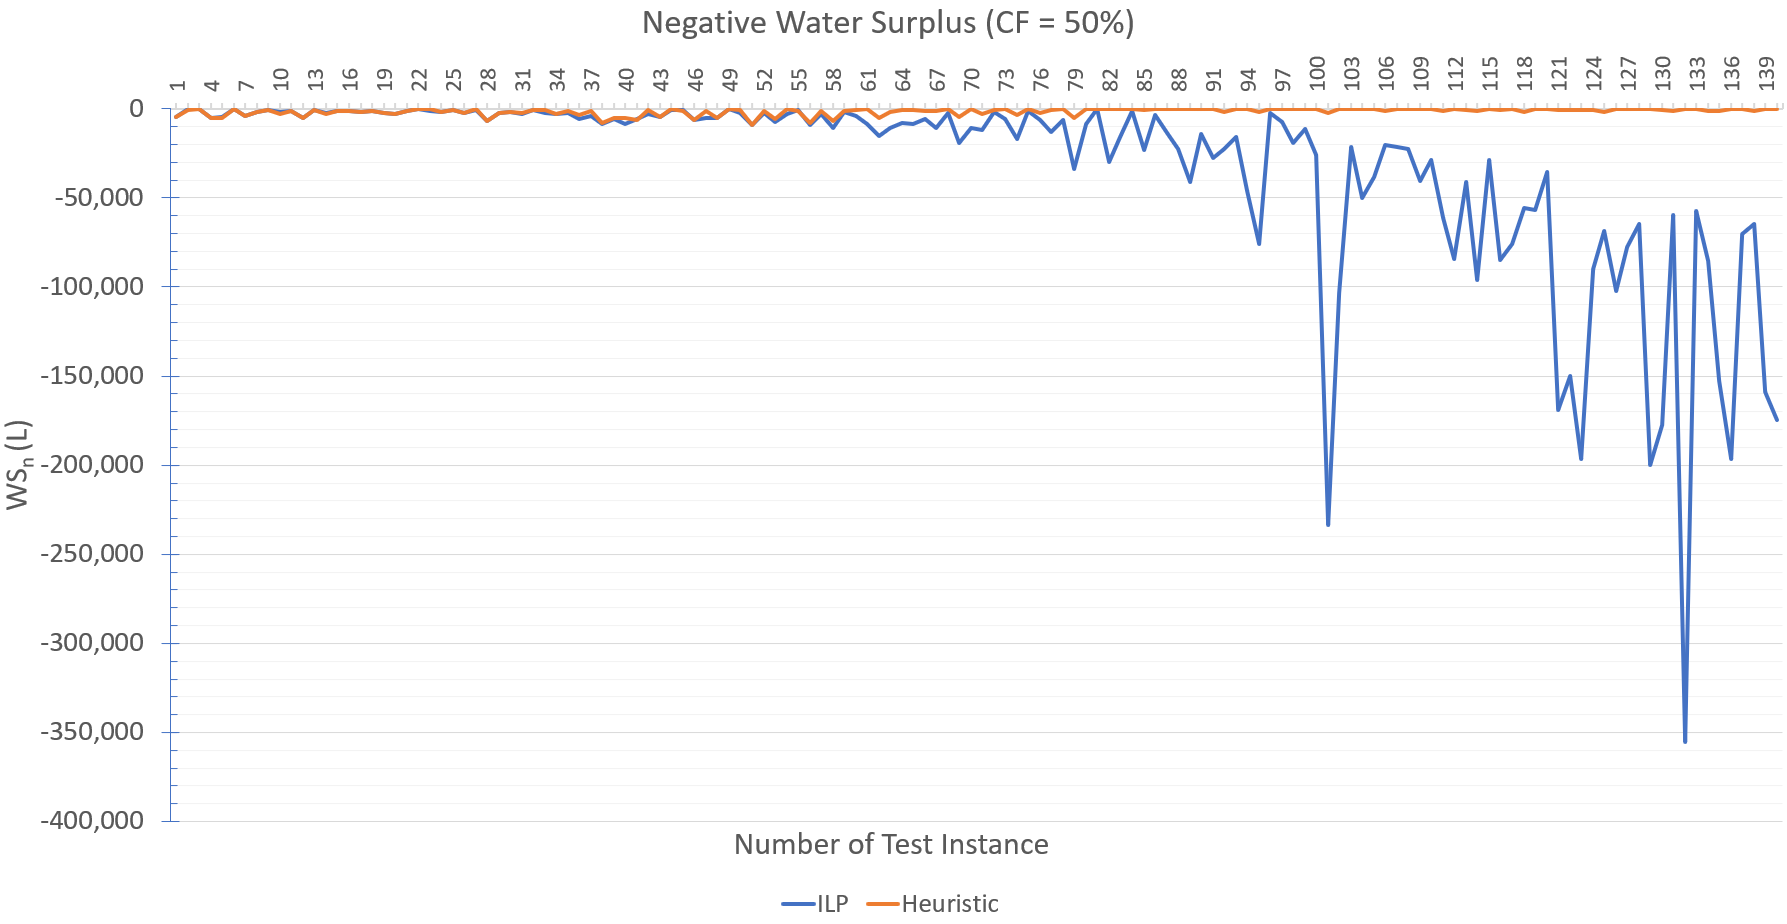
\includegraphics[width=\linewidth]{img/wsn-cf50.png}
    \caption{Comparison of negative water surplus per test instance for $\mathit{CF} = 50\%$}
    \label{fig:wsn-cf50}
\end{figure}

To get a better idea of the obtained results, Figure~\ref{fig:wsn-cf50} depicts the negative water surplus in the solutions obtained by the heuristic and ILP approaches, for each $\mathit{CF} = 50\%$ test instance.
The 140 test instances are ordered by increasing size, as if Table~\ref{tbl:comparison-cf-50} were read row by row, with the size increasing every 20 instances.
Note the scale on the vertical axis -- the negative water surplus of ILP solutions reaches hundreds of thousands of liters, while heuristic solutions stay firmly within ten thousand liters (corresponding to 2--3 drops for airtankers or heavy helicopters, or around 10 drops for light helicopters).

The relative optimality gap in CPLEX was set to $10^{-4}$, meaning that it is unlikely $\mathit{WO}$ will be optimal as it barely had any effect on the value of the objective function, and, if the absolute value of $\mathit{WS_n}$ is large, $\mathit{Z}$ might also be suboptimal, but should be fairly close.
This is the reason why, in some rare cases, the heuristic algorithm can find a better solution than what CPLEX considers to be optimal.
For example, the K07\_F02 UOF + MUOT scenarios for $\mathit{CF} = 15\%$ and $\mathit{CF} = 50\%$, and the K07\_F02 NUOF + MUOT $\mathit{CF} = 25\%$ scenario.
It is also possible that the heuristic algorithm found some optimal solutions which the ILP approach did not manage to find, however, we cannot know that for sure.

Instances with a higher $\mathit{CF}$ value have approximately uniformly higher target water content per time slot than those with a lower value.
Having very little negative water surplus in instances with a high $\mathit{CF}$ value is much more important, as it means a more uniform distribution of water was achieved for a similar total water output.
However, setting a very high $\mathit{CF}$ value (e.g., $90\%$) leads to very large absolute values of negative water surplus because it is impossible to schedule resources such that the targets are close to being satisfied.
This also often results in a large absolute value of minimal water surplus, sometimes completely ignoring several time slots, and entirely missing the goal of achieving a continuous flow of water.
As can be seen from Table~\ref{tbl:comparison-cf-50}, approximately $\mathit{CF} = 50\%$ seems to be a reasonable choice because the negative water surplus is often very close to zero.
Of course, in real-world scenarios the incident commander determines the required target water content, but their decision should be grounded on similar principles so as not to lead to unsatisfying solutions.
It should also be noted that the heuristic algorithm outperforms the ILP approach by a growing margin as $\mathit{CF}$ increases, as well as beginning to outperform ILP for smaller instances.

There seems to very little difference in solution quality for different target water content distributions over time and fronts, indicating that the heuristic algorithm is robust.
The differences are not consistent, and the relative performance for a certain distribution changes for different $\mathit{CF}$ values and scenario sizes.
This is likely due to the random nature of the test scenarios.
Perhaps some groups of scenarios had slightly higher targets and simulated worse flying conditions (reduced number of drops per hour), resulting in relatively worse solution quality.

As expected, local search always improves the solutions found by the randomized greedy algorithm.
It should be noted that, for $\mathit{CF} = 50\%$ and scenarios with 20 or more aerial resources, the greedy algorithm manages to beat the ILP approach in averaged objective values.
More precisely, it beats the ILP solutions in 72 of the 80 test instances.

For larger test instances, the randomized greedy algorithm takes approximately a third of the total execution time.
Of course, the exact ratio depends on the duration of the local search, i.e., the number of iterations $L$.
For smaller instances, the greedy algorithm finishes practically instantly.

Unfortunately, the performance of the heuristic algorithm does not improve linearly with the number of used threads.
Employing more threads, up to the number of available cores, will increase the number of performed GRASP iterations per unit of time, but will also slow down individual iterations, increasing their duration.
Therefore, the durations shown in Table~\ref{tbl:iteration-time} depict the worst-case scenario, and allow for realistic calculations of what the execution time would be for a large number of threads and iterations.
For example, for K35\_F05, 200 GRASP iterations, and 20 threads, each thread would execute 10 GRASP iterations, resulting in an execution time of approximately \SI{146}{\second}.
If a CPU with eight threads were used, it can be expected that the execution would take \SI{366}{\second}, or approximately six minutes, assuming that the processor has similar single-threaded performance as the 3900X.
If a single worker thread were used, the GRASP iteration duration would be reduced by approximately $35\%$ (measured for K35\_F05), bringing the time down to about \SI{9.5}{\second} per iteration.
Of course, it is more beneficial to perform more GRASP iterations in a predetermined amount of time, which is why using as many worker threads as reasonably possible is recommended.
In most cases, the number of worker threads should be equal to the number of logical processors.

Rudimentary testing was performed on instances outside of the scope of the defined test scenarios.
Specifically, test instances with 50 aerial resources, five fire fronts, and $\mathit{CF} = 50\%$ were used.
For the same parameters as in Table~\ref{tbl:iteration-time}, an average GRASP duration took approximately \SI{25.2}{\second}, divided into \SI{14.8}{\second} for the randomized greedy algorithm, and \SI{10.4}{\second} for local search.

Not only is the heuristic algorithm very fast, but it also uses very little memory (RAM).
For largest tested instances (K35\_F05), it reported using approximately $\SI{1}{\mega\byte} + w \cdot \SI{0.5}{\mega\byte}$ of memory, where $w$ is the number of worker threads in a thread pool.
On the other hand, the ILP approach occasionally used more than \SI{900}{\mega\byte} of RAM with 16 active threads.
With respect to the CPU usage, the number of worker threads can be specified for both approaches, making them scalable with the number of CPU cores, and therefore tied in that regard.

Table~\ref{tbl:comparison-extended} provides a comparison of ILP solutions found after six hours using a more powerful CPU, and the solutions found by the heuristic algorithm.
It can be seen that, in most cases, the heuristic algorithm will still prevail in quality, doing so in mere seconds per GRASP iteration.
ILP solutions have higher quality only for smaller instances and $\mathit{CF} = 15\%$, which is less important, and it is truly not a significant difference.
It most certainly does not justify the required execution time.
To reiterate, the heuristic algorithm found the solutions shown in Table~\ref{tbl:comparison-extended} in less than 150 seconds per problem instance (elapsed real time), on the same hardware where the linear solver was executed.
Each instance with 15 or 20 resources was solved within one minute.


\section{Hyperparameter Values}

Detailed analysis of the effects of hyperparameter values (function arguments in Algorithm~\ref{alg:grasp}) was not conducted.
From rudimentary testing it was concluded that very different values of parameters still perform remarkably well.
Also, performance depends on the specific instance -- some values might achieve better results with one instance, and worse with another.
Default values, as shown in Table~\ref{tbl:cli}, have been found to work quite well.

Generally speaking, higher numbers of GRASP and local search iterations may lead to better solutions, with diminishing returns after approximately $100$ and $7\,000$ iterations, respectively, depending on the instance size.
In some smaller instances, optimal solutions were found withing a dozen GRASP iterations.
For small instances, a couple thousand local search iterations should be more than enough.
Obviously, a larger number of iterations will increase the execution time, doing so approximately linearly.

As a rule of thumb, $N_D - N_R \le 2$ should hold.
Otherwise, the search will be slowed down significantly due to the extensive use of optimal depth-first search, with a minimal benefit to the solution quality.
It would be better to spend the time on executing more iterations than on deepened DFS.
If DFS wants to be completely avoided, the hyperparameters can be set such that $N_R \gg N_D$.

The optimal starting temperature heavily depends on the values of the weighting factors in the objective function, and the expected negative water surplus, which in turn define the expected values of the objective function.
In practice, it is a good idea to initially have approximately $50\%$ chance of accepting non-improving solutions, resulting in $T_0 \approx -1.5 \, \cdot \, \Delta f$.
The expected average value of $\Delta f$ is an open question, and depends on the problem instance.
It should not be a big issue if $T_0$ is larger than described, as that will only result in a more randomized search at the beginning, which is not necessarily a bad thing.
After $L$ local search iterations, the final temperature will be $T_L = \beta ^ L \cdot T_0$.
If one already has a final temperature in mind, the equation can be reversed in order to calculate the required cooling factor: $\beta = \log_L \left( T_L \, / \, T_0 \right)$.
If $a_1 \gg a_2 \gg a_3$ holds, and the target water content can be almost satisfied for a particular problem instance, then $T_L \in [ a_3, a_2 ]$ is a reasonable target value for the final temperature.

Weighting factors used in the greedy construction phase and the repair method ($k_{r, G}, k_{p, G}, k_{r, R}, k_{p, R}$) are particularly prone to noticeably altering the solution quality when modified.
For some instances smaller values work best, and for others it is beneficial to set them to values upwards of $10$, completely overshadowing the objective function (Algorithm~\ref{alg:greedy}, line~\ref{alg:greedy-line-fitness-def}).
Factors $k_{p, G}$ and $k_{p, R}$ should not be set close to zero if $N_R \not\gg N_D$, as that can lead to intermediate schedules which have a lot of unscheduled flights when compared to the maximum possible number of takeoffs, resulting in DFS significantly slowing down the entire search because the search depth will be much larger than expected.
If some GRASP iterations seem to take much longer than others, it might be due to DFS, and increasing $N_D$ should help resolve that problem.

Considering that a GRASP iteration can be performed within seconds, even in case of largest test instances, it is a good idea to restart the search multiple times, each time using different parameters.
Using a CPU with eight logical processors, a test scenario with 20 aerial resources can be solved ten times over within ten minutes, each time executing almost a hundred GRASP iterations.
This way, the heuristic algorithm will be used to its full potential.

\chapter{Future Work}

As is the case for many models, and especially heuristic algorithms, there is room for improvement.
A number of potential modifications is presented, which should all lead to improved solution quality in terms of the objective function value and/or fire suppression effectiveness in real scenarios.


\section{Model}

If permitted by legislation, the model could be extended to allow for flights with long transit times to start or end at night-time.
This could greatly help with alleviating the problem of unsatisfied target water content in the first and last slot of the day.

The objective function could be changed to better reflect the need for a uniform distribution of the water surplus.
The original objective function presented in Equation \ref{eq:objective} does not address how the negative water surplus is distributed over fronts.
One option could be to use Equation \ref{eq:alternative-objective-squared} as the objective function:
\begin{equation}\label{eq:alternative-objective-squared}
\max \left( - a_1 \cdot \sum_{f \in \mathcal{F}} \left( \sum_{t \in \mathcal{T}} \min ( \mathit{WS}_{tf}, 0 ) \right) ^ 2
    + a_2 \cdot Z
    + a_3 \cdot \mathit{WO} \right)
\end{equation}
By grouping the negative water surplus for each front and squaring the sum, the value of the objective function would be lower if the same amount of negative water surplus was concentrated on fewer fronts.
Another option could be to minimize the variance of water surplus.
However, if precautions are not taken, it could result in reduced total water output and overall worse solutions.
A downside of described modifications is that the model stops being linear, but that should not be a hurdle for a heuristic algorithm.

Furthermore, water surplus could be measured as a percentage of the water target for every slot, instead of an absolute value.
That would help with disproportionate neglect of fire fronts which require less water, as the punishment would be greater.

Lastly, it is reasonable to assume that having negative water surplus in consecutive time slots is worse than if it were sporadically spread throughout the day, with all other things being equal.
Grouped negative water surplus will be detrimental to the suppression efforts because the wildfire will have a bigger time window in which it can spread, possibly requiring more resources than expected in the future.
It would be beneficial to have penalties incorporated into the objective function for such consecutive shortfalls.


\section{Heuristic Algorithm}

Tabu search was often successfully employed in scheduling problems~\cite{Brandimarte/TS}\cite{Dell/TS}.
Combining tabu search with the existing algorithm could help it escape local optima.
For example, takeoffs which were inserted as a part of the \textit{repair} process are entered into the tabu list.
The \textit{destroy} method is then not allowed to remove any takeoff which is in the tabu list.
The tabu tenure would have to be added as a new hyperparameter.
In a similar effort, guided local search could be used to modify the parameters as the search progresses~\cite{Voudouris/GLS}.

In the \textit{destroy} method of large neighborhood search it might be beneficial to find potential takeoffs which could significantly improve the value of the objective function, but are blocked.
However, if they are blocked only by one or two existing takeoffs, then those takeoffs could be removed and repairs conducted as usual.
That would make the search more directed at the expense of more complicated implementation.
Specifically, for every potential takeoff we would need to cache which takeoffs are blocking it.

While building the initial greedy solution, perhaps it is beneficial to forcefully assign flights which meet the requirements of the first and last time slots.
It is not certain that in the optimal solution those slots will indeed have their requirements met, but it might be a reasonable starting move.

\chapter{Conclusion}

In this thesis, we devise and implement a fast heuristic search algorithm for efficient scheduling of aerial resources, namely helicopters and airplanes, in order to maximize the wildfire suppression via aerial firefighting.
The focus is put on tackling large-scale wildfires divided into multiple fire fronts, where a total of approximately 20 or more aerial resources are involved.
Furthermore, Spanish aviation regulations are taken into consideration, as well as limitations on the number and type of aircraft allowed to fly at one front at the same time.

The parallelized heuristic algorithm is based on the greedy randomized adaptive search procedure (GRASP) combined with large neighborhood search and simulated annealing, thus efficiently navigating a vast solution space in polynomial time complexity.
The implementation is done in the C++ programming language in order to achieve maximum performance.

The heuristic algorithm is evaluated on a set of 420 test instances, divided into 84 scenarios with varying size and distribution of the target water content.
Compared to the integer linear programming (ILP) model, executed with a time limit of two hours, the heuristic algorithm consistently obtains solutions of substantially higher quality in a fraction of the time, especially in case of large and very large scenarios, as well as scenarios with increased target water content.
For smaller scenarios, the heuristic algorithm regularly finds near-optimal solutions.
Furthermore, it found optimal solutions in $75\%$ of instances for which ILP also reported finding the optimal solution.
Unlike the ILP approach, the heuristic algorithm is highly scalable, running in under 15 seconds per GRASP iteration for every test instance, and under five minutes for the entire search procedure, while using approximately 100 times less memory than the ILP solver.

Very promising performance of the heuristic algorithm makes it an excellent alternative for the ILP approach.

The source code and all other relevant materials are made available in a public \textit{GitHub} repository: \small{\url{https://github.com/LMesaric/MSc-Thesis-FER-2022}}.


\renewcommand\bibname{References}
\bibliographystyle{ieeetr}
\bibliography{literature}

\appendix
\chapter{Example of AMPL Input Data Format}\label{appx:input-file-ampl}

\lstset{style=appendix-file-style}
\begin{lstlisting}
data;
set K:= K1 K2 K3 K4 K5 K6 K7 ;

set F:= F1 F2 ;

set Q:= Q1 Q2 ;

param T:= 45;
param V:
	K1  K2  K3  K4  K5  K6  K7  :=
Q1	1   1   1   1   0   0   0
Q2	0   0   0   0   1   1   1
; # if resource k is of type q

param TF:=
K1 6
K2 6
K3 6
K4 6
K5 12
K6 12
K7 12
; # number of continuous time slots resource can fly

param TR:=
K1 2
K2 2
K3 2
K4 2
K5 4
K6 4
K7 4
; # number of continuous time slots resource k needs to rest between flights

param P:=
K1 36
K2 36
K3 36
K4 36
K5 36
K6 36
K7 36
; # number of continuous time slots a pilot can be present including rest times for resource k

param N:=
K1 4
K2 4
K3 4
K4 4
K5 1
K6 2
K7 2
; # max number of flights resource k can fly in the total time period

param A:
	K1  K2  K3  K4  K5  K6  K7  :=
1	1   1   1   1   0   1   1
2	1   1   1   1   0   1   1
3	1   1   1   1   0   1   1
4	1   1   1   1   0   1   1
5	1   1   1   1   0   1   1
6	1   1   1   1   0   1   1
7	1   1   1   1   0   1   1
8	1   1   1   1   0   1   1
9	1   1   1   1   0   1   1
10	1   1   1   1   0   1   1
11	1   1   1   1   0   1   1
12	1   1   1   1   0   1   1
13	1   1   1   1   0   1   1
14	1   1   1   1   0   1   1
15	1   1   1   1   0   1   1
16	1   1   1   1   0   1   1
17	1   1   1   1   1   1   1
18	1   1   1   1   1   1   1
19	1   1   1   1   1   1   1
20	1   1   1   1   1   1   1
21	1   1   1   1   1   1   1
22	1   1   1   1   1   1   1
23	1   1   1   1   1   1   1
24	1   1   1   1   1   1   1
25	1   1   1   1   1   1   1
26	1   1   1   1   1   1   1
27	1   1   1   1   1   1   1
28	1   1   1   1   1   1   1
29	1   1   1   1   1   1   1
30	1   1   1   1   1   1   1
31	1   1   1   1   1   1   1
32	1   1   1   1   1   1   1
33	1   1   1   1   1   1   1
34	1   1   1   1   1   1   1
35	1   1   1   1   1   1   1
36	1   1   1   1   1   1   1
37	1   1   1   1   1   1   1
38	1   1   1   1   1   1   1
39	1   1   1   1   1   1   1
40	1   1   1   1   1   1   1
41	1   1   1   1   1   1   1
42	1   1   1   1   1   1   1
43	1   1   1   1   1   1   1
44	1   1   1   1   1   1   1
45	1   1   1   1   1   1   1
; # availability of resource k in time slot t

param B:
	F1  F2  :=
Q1	1   0
Q2	0   0
; # if front f requires resources of type q

param U:
	F1  F2  :=
K1	0   0
K2	0   0
K3	0   0
K4	0   0
K5	2   2
K6	0   0
K7	0   0
; # transit time of resource

param C:=
K1 900
K2 900
K3 1500
K4 4500
K5 5500
K6 5500
K7 5500
; #  water capacity of resource k

param S:=
F1 9
F2 7
; # max number of resources that can fly at front f in the same time slot

param D:=

[*,*,F1 ]:  K1    K2    K3    K4    K5    K6    K7    :=
1           1.37  1.37  1.37  1.09  0.82  0.82  0.82
2           1.37  1.37  1.37  1.09  0.82  0.82  0.82
3           1.37  1.37  1.37  1.09  0.82  0.82  0.82
4           1.37  1.37  1.37  1.09  0.82  0.82  0.82
5           1.37  1.37  1.37  1.09  0.82  0.82  0.82
6           1.37  1.37  1.37  1.09  0.82  0.82  0.82
7           1.37  1.37  1.37  1.09  0.82  0.82  0.82
8           1.37  1.37  1.37  1.09  0.82  0.82  0.82
9           1.37  1.37  1.37  1.09  0.82  0.82  0.82
10          1.37  1.37  1.37  1.09  0.82  0.82  0.82
11          1.37  1.37  1.37  1.09  0.82  0.82  0.82
12          1.37  1.37  1.37  1.09  0.82  0.82  0.82
13          1.37  1.37  1.37  1.09  0.82  0.82  0.82
14          1.37  1.37  1.37  1.09  0.82  0.82  0.82
15          1.37  1.37  1.37  1.09  0.82  0.82  0.82
16          1.37  1.37  1.37  1.09  0.82  0.82  0.82
17          1.37  1.37  1.37  1.09  0.82  0.82  0.82
18          1.37  1.37  1.37  1.09  0.82  0.82  0.82
19          1.37  1.37  1.37  1.09  0.82  0.82  0.82
20          1.37  1.37  1.37  1.09  0.82  0.82  0.82
21          1.37  1.37  1.37  1.09  0.82  0.82  0.82
22          1.37  1.37  1.37  1.09  0.82  0.82  0.82
23          1.37  1.37  1.37  1.09  0.82  0.82  0.82
24          1.37  1.37  1.37  1.09  0.82  0.82  0.82
25          1.30  1.30  1.30  1.04  0.78  0.78  0.78
26          1.30  1.30  1.30  1.04  0.78  0.78  0.78
27          1.30  1.30  1.30  1.04  0.78  0.78  0.78
28          1.30  1.30  1.30  1.04  0.78  0.78  0.78
29          1.30  1.30  1.30  1.04  0.78  0.78  0.78
30          1.30  1.30  1.30  1.04  0.78  0.78  0.78
31          1.30  1.30  1.30  1.04  0.78  0.78  0.78
32          1.30  1.30  1.30  1.04  0.78  0.78  0.78
33          1.30  1.30  1.30  1.04  0.78  0.78  0.78
34          1.37  1.37  1.37  1.09  0.82  0.82  0.82
35          1.37  1.37  1.37  1.09  0.82  0.82  0.82
36          1.37  1.37  1.37  1.09  0.82  0.82  0.82
37          1.37  1.37  1.37  1.09  0.82  0.82  0.82
38          1.37  1.37  1.37  1.09  0.82  0.82  0.82
39          1.37  1.37  1.37  1.09  0.82  0.82  0.82
40          1.37  1.37  1.37  1.09  0.82  0.82  0.82
41          1.37  1.37  1.37  1.09  0.82  0.82  0.82
42          1.37  1.37  1.37  1.09  0.82  0.82  0.82
43          1.37  1.37  1.37  1.09  0.82  0.82  0.82
44          1.37  1.37  1.37  1.09  0.82  0.82  0.82
45          1.37  1.37  1.37  1.09  0.82  0.82  0.82

[*,*,F2 ]:  K1    K2    K3    K4    K5    K6    K7    :=
1           1.62  1.62  1.62  1.29  0.97  0.97  0.97
2           1.62  1.62  1.62  1.29  0.97  0.97  0.97
3           1.62  1.62  1.62  1.29  0.97  0.97  0.97
4           1.62  1.62  1.62  1.29  0.97  0.97  0.97
5           1.62  1.62  1.62  1.29  0.97  0.97  0.97
6           1.62  1.62  1.62  1.29  0.97  0.97  0.97
7           1.62  1.62  1.62  1.29  0.97  0.97  0.97
8           1.62  1.62  1.62  1.29  0.97  0.97  0.97
9           1.62  1.62  1.62  1.29  0.97  0.97  0.97
10          1.62  1.62  1.62  1.29  0.97  0.97  0.97
11          1.62  1.62  1.62  1.29  0.97  0.97  0.97
12          1.62  1.62  1.62  1.29  0.97  0.97  0.97
13          1.62  1.62  1.62  1.29  0.97  0.97  0.97
14          1.62  1.62  1.62  1.29  0.97  0.97  0.97
15          1.62  1.62  1.62  1.29  0.97  0.97  0.97
16          1.62  1.62  1.62  1.29  0.97  0.97  0.97
17          1.62  1.62  1.62  1.29  0.97  0.97  0.97
18          1.62  1.62  1.62  1.29  0.97  0.97  0.97
19          1.62  1.62  1.62  1.29  0.97  0.97  0.97
20          1.62  1.62  1.62  1.29  0.97  0.97  0.97
21          1.62  1.62  1.62  1.29  0.97  0.97  0.97
22          1.62  1.62  1.62  1.29  0.97  0.97  0.97
23          1.62  1.62  1.62  1.29  0.97  0.97  0.97
24          1.62  1.62  1.62  1.29  0.97  0.97  0.97
25          1.54  1.54  1.54  1.23  0.92  0.92  0.92
26          1.54  1.54  1.54  1.23  0.92  0.92  0.92
27          1.54  1.54  1.54  1.23  0.92  0.92  0.92
28          1.54  1.54  1.54  1.23  0.92  0.92  0.92
29          1.54  1.54  1.54  1.23  0.92  0.92  0.92
30          1.54  1.54  1.54  1.23  0.92  0.92  0.92
31          1.54  1.54  1.54  1.23  0.92  0.92  0.92
32          1.54  1.54  1.54  1.23  0.92  0.92  0.92
33          1.54  1.54  1.54  1.23  0.92  0.92  0.92
34          1.62  1.62  1.62  1.29  0.97  0.97  0.97
35          1.62  1.62  1.62  1.29  0.97  0.97  0.97
36          1.62  1.62  1.62  1.29  0.97  0.97  0.97
37          1.62  1.62  1.62  1.29  0.97  0.97  0.97
38          1.62  1.62  1.62  1.29  0.97  0.97  0.97
39          1.62  1.62  1.62  1.29  0.97  0.97  0.97
40          1.62  1.62  1.62  1.29  0.97  0.97  0.97
41          1.62  1.62  1.62  1.29  0.97  0.97  0.97
42          1.62  1.62  1.62  1.29  0.97  0.97  0.97
43          1.62  1.62  1.62  1.29  0.97  0.97  0.97
44          1.62  1.62  1.62  1.29  0.97  0.97  0.97
45          1.62  1.62  1.62  1.29  0.97  0.97  0.97
; # number of drops resource k can do at front f in time slot t if it is a firefighting time slot

param E:=

[*,*,F1 ]:  K1    K2    K3    K4    K5    K6    K7    :=
1           0.22  0.41  0.15  0.07  0.28  0.11  0.11
2           0.22  0.41  0.15  0.07  0.28  0.11  0.11
3           0.22  0.41  0.15  0.07  0.28  0.11  0.11
4           0.22  0.41  0.15  0.07  0.28  0.11  0.11
5           0.22  0.41  0.15  0.07  0.28  0.11  0.11
6           0.22  0.41  0.15  0.07  0.28  0.11  0.11
7           0.22  0.41  0.15  0.07  0.28  0.11  0.11
8           0.22  0.41  0.15  0.07  0.28  0.11  0.11
9           0.22  0.41  0.15  0.07  0.28  0.11  0.11
10          0.22  0.41  0.15  0.07  0.28  0.11  0.11
11          0.22  0.41  0.15  0.07  0.28  0.11  0.11
12          0.22  0.41  0.15  0.07  0.28  0.11  0.11
13          0.22  0.41  0.15  0.07  0.28  0.11  0.11
14          0.22  0.41  0.15  0.07  0.28  0.11  0.11
15          0.22  0.41  0.15  0.07  0.28  0.11  0.11
16          0.22  0.41  0.15  0.07  0.28  0.11  0.11
17          0.22  0.41  0.15  0.07  0.28  0.11  0.11
18          0.22  0.41  0.15  0.07  0.28  0.11  0.11
19          0.22  0.41  0.15  0.07  0.28  0.11  0.11
20          0.22  0.41  0.15  0.07  0.28  0.11  0.11
21          0.22  0.41  0.15  0.07  0.28  0.11  0.11
22          0.22  0.41  0.15  0.07  0.28  0.11  0.11
23          0.22  0.41  0.15  0.07  0.28  0.11  0.11
24          0.22  0.41  0.15  0.07  0.28  0.11  0.11
25          0.21  0.39  0.14  0.06  0.26  0.11  0.10
26          0.21  0.39  0.14  0.06  0.26  0.11  0.10
27          0.21  0.39  0.14  0.06  0.26  0.11  0.10
28          0.21  0.39  0.14  0.06  0.26  0.11  0.10
29          0.21  0.39  0.14  0.06  0.26  0.11  0.10
30          0.21  0.39  0.14  0.06  0.26  0.11  0.10
31          0.21  0.39  0.14  0.06  0.26  0.11  0.10
32          0.21  0.39  0.14  0.06  0.26  0.11  0.10
33          0.21  0.39  0.14  0.06  0.26  0.11  0.10
34          0.22  0.41  0.15  0.07  0.28  0.11  0.11
35          0.22  0.41  0.15  0.07  0.28  0.11  0.11
36          0.22  0.41  0.15  0.07  0.28  0.11  0.11
37          0.22  0.41  0.15  0.07  0.28  0.11  0.11
38          0.22  0.41  0.15  0.07  0.28  0.11  0.11
39          0.22  0.41  0.15  0.07  0.28  0.11  0.11
40          0.22  0.41  0.15  0.07  0.28  0.11  0.11
41          0.22  0.41  0.15  0.07  0.28  0.11  0.11
42          0.22  0.41  0.15  0.07  0.28  0.11  0.11
43          0.22  0.41  0.15  0.07  0.28  0.11  0.11
44          0.22  0.41  0.15  0.07  0.28  0.11  0.11
45          0.22  0.41  0.15  0.07  0.28  0.11  0.11

[*,*,F2 ]:  K1    K2    K3    K4    K5    K6    K7    :=
1           0.23  0.47  0.24  0.08  0.36  0.18  0.22
2           0.23  0.47  0.24  0.08  0.36  0.18  0.22
3           0.23  0.47  0.24  0.08  0.36  0.18  0.22
4           0.23  0.47  0.24  0.08  0.36  0.18  0.22
5           0.23  0.47  0.24  0.08  0.36  0.18  0.22
6           0.23  0.47  0.24  0.08  0.36  0.18  0.22
7           0.23  0.47  0.24  0.08  0.36  0.18  0.22
8           0.23  0.47  0.24  0.08  0.36  0.18  0.22
9           0.23  0.47  0.24  0.08  0.36  0.18  0.22
10          0.23  0.47  0.24  0.08  0.36  0.18  0.22
11          0.23  0.47  0.24  0.08  0.36  0.18  0.22
12          0.23  0.47  0.24  0.08  0.36  0.18  0.22
13          0.23  0.47  0.24  0.08  0.36  0.18  0.22
14          0.23  0.47  0.24  0.08  0.36  0.18  0.22
15          0.23  0.47  0.24  0.08  0.36  0.18  0.22
16          0.23  0.47  0.24  0.08  0.36  0.18  0.22
17          0.23  0.47  0.24  0.08  0.36  0.18  0.22
18          0.23  0.47  0.24  0.08  0.36  0.18  0.22
19          0.23  0.47  0.24  0.08  0.36  0.18  0.22
20          0.23  0.47  0.24  0.08  0.36  0.18  0.22
21          0.23  0.47  0.24  0.08  0.36  0.18  0.22
22          0.23  0.47  0.24  0.08  0.36  0.18  0.22
23          0.23  0.47  0.24  0.08  0.36  0.18  0.22
24          0.23  0.47  0.24  0.08  0.36  0.18  0.22
25          0.22  0.45  0.23  0.07  0.34  0.18  0.21
26          0.22  0.45  0.23  0.07  0.34  0.18  0.21
27          0.22  0.45  0.23  0.07  0.34  0.18  0.21
28          0.22  0.45  0.23  0.07  0.34  0.18  0.21
29          0.22  0.45  0.23  0.07  0.34  0.18  0.21
30          0.22  0.45  0.23  0.07  0.34  0.18  0.21
31          0.22  0.45  0.23  0.07  0.34  0.18  0.21
32          0.22  0.45  0.23  0.07  0.34  0.18  0.21
33          0.22  0.45  0.23  0.07  0.34  0.18  0.21
34          0.23  0.47  0.24  0.08  0.36  0.18  0.22
35          0.23  0.47  0.24  0.08  0.36  0.18  0.22
36          0.23  0.47  0.24  0.08  0.36  0.18  0.22
37          0.23  0.47  0.24  0.08  0.36  0.18  0.22
38          0.23  0.47  0.24  0.08  0.36  0.18  0.22
39          0.23  0.47  0.24  0.08  0.36  0.18  0.22
40          0.23  0.47  0.24  0.08  0.36  0.18  0.22
41          0.23  0.47  0.24  0.08  0.36  0.18  0.22
42          0.23  0.47  0.24  0.08  0.36  0.18  0.22
43          0.23  0.47  0.24  0.08  0.36  0.18  0.22
44          0.23  0.47  0.24  0.08  0.36  0.18  0.22
45          0.23  0.47  0.24  0.08  0.36  0.18  0.22
; # number of drops resource k can do at front f in time slot t if starting or ending flight

param W:
	F1        F2        :=
1	314.56    169.38
2	1258.23   677.51
3	1258.23   677.51
4	1258.23   677.51
5	1258.23   677.51
6	1258.23   677.51
7	1258.23   677.51
8	1258.23   677.51
9	1258.23   677.51
10	1258.23   677.51
11	1258.23   677.51
12	1258.23   677.51
13	1258.23   677.51
14	1258.23   677.51
15	1258.23   677.51
16	1258.23   677.51
17	1258.23   677.51
18	1258.23   677.51
19	559.21    301.11
20	559.21    301.11
21	559.21    301.11
22	559.21    301.11
23	559.21    301.11
24	559.21    301.11
25	559.21    301.11
26	559.21    301.11
27	559.21    301.11
28	559.21    301.11
29	559.21    301.11
30	559.21    301.11
31	559.21    301.11
32	559.21    301.11
33	559.21    301.11
34	559.21    301.11
35	559.21    301.11
36	559.21    301.11
37	559.21    301.11
38	559.21    301.11
39	559.21    301.11
40	559.21    301.11
41	559.21    301.11
42	559.21    301.11
43	559.21    301.11
44	559.21    301.11
45	139.80    75.28
; # water needed at front f in time slot t

param M := 100000000;

param a1:= 10000000;

param a2:= 100;

param a3:= 0.0001;
\end{lstlisting}

\chapter{Example of Simple Input Data Format}\label{appx:input-file-simple}

\lstset{style=appendix-file-style}
\begin{lstlisting}
7 2 45

1 1 1 1 0 0 0

6 6 6 6 12 12 12

2 2 2 2 4 4 4

36 36 36 36 36 36 36

4 4 4 4 1 2 2

1 1 1 1 0 1 1
1 1 1 1 0 1 1
1 1 1 1 0 1 1
1 1 1 1 0 1 1
1 1 1 1 0 1 1
1 1 1 1 0 1 1
1 1 1 1 0 1 1
1 1 1 1 0 1 1
1 1 1 1 0 1 1
1 1 1 1 0 1 1
1 1 1 1 0 1 1
1 1 1 1 0 1 1
1 1 1 1 0 1 1
1 1 1 1 0 1 1
1 1 1 1 0 1 1
1 1 1 1 0 1 1
1 1 1 1 1 1 1
1 1 1 1 1 1 1
1 1 1 1 1 1 1
1 1 1 1 1 1 1
1 1 1 1 1 1 1
1 1 1 1 1 1 1
1 1 1 1 1 1 1
1 1 1 1 1 1 1
1 1 1 1 1 1 1
1 1 1 1 1 1 1
1 1 1 1 1 1 1
1 1 1 1 1 1 1
1 1 1 1 1 1 1
1 1 1 1 1 1 1
1 1 1 1 1 1 1
1 1 1 1 1 1 1
1 1 1 1 1 1 1
1 1 1 1 1 1 1
1 1 1 1 1 1 1
1 1 1 1 1 1 1
1 1 1 1 1 1 1
1 1 1 1 1 1 1
1 1 1 1 1 1 1
1 1 1 1 1 1 1
1 1 1 1 1 1 1
1 1 1 1 1 1 1
1 1 1 1 1 1 1
1 1 1 1 1 1 1
1 1 1 1 1 1 1

1 0

0 0
0 0
0 0
0 0
2 2
0 0
0 0

900 900 1500 4500 5500 5500 5500

9 7

1.37  1.37  1.37  1.09  0.82  0.82  0.82
1.37  1.37  1.37  1.09  0.82  0.82  0.82
1.37  1.37  1.37  1.09  0.82  0.82  0.82
1.37  1.37  1.37  1.09  0.82  0.82  0.82
1.37  1.37  1.37  1.09  0.82  0.82  0.82
1.37  1.37  1.37  1.09  0.82  0.82  0.82
1.37  1.37  1.37  1.09  0.82  0.82  0.82
1.37  1.37  1.37  1.09  0.82  0.82  0.82
1.37  1.37  1.37  1.09  0.82  0.82  0.82
1.37  1.37  1.37  1.09  0.82  0.82  0.82
1.37  1.37  1.37  1.09  0.82  0.82  0.82
1.37  1.37  1.37  1.09  0.82  0.82  0.82
1.37  1.37  1.37  1.09  0.82  0.82  0.82
1.37  1.37  1.37  1.09  0.82  0.82  0.82
1.37  1.37  1.37  1.09  0.82  0.82  0.82
1.37  1.37  1.37  1.09  0.82  0.82  0.82
1.37  1.37  1.37  1.09  0.82  0.82  0.82
1.37  1.37  1.37  1.09  0.82  0.82  0.82
1.37  1.37  1.37  1.09  0.82  0.82  0.82
1.37  1.37  1.37  1.09  0.82  0.82  0.82
1.37  1.37  1.37  1.09  0.82  0.82  0.82
1.37  1.37  1.37  1.09  0.82  0.82  0.82
1.37  1.37  1.37  1.09  0.82  0.82  0.82
1.37  1.37  1.37  1.09  0.82  0.82  0.82
1.30  1.30  1.30  1.04  0.78  0.78  0.78
1.30  1.30  1.30  1.04  0.78  0.78  0.78
1.30  1.30  1.30  1.04  0.78  0.78  0.78
1.30  1.30  1.30  1.04  0.78  0.78  0.78
1.30  1.30  1.30  1.04  0.78  0.78  0.78
1.30  1.30  1.30  1.04  0.78  0.78  0.78
1.30  1.30  1.30  1.04  0.78  0.78  0.78
1.30  1.30  1.30  1.04  0.78  0.78  0.78
1.30  1.30  1.30  1.04  0.78  0.78  0.78
1.37  1.37  1.37  1.09  0.82  0.82  0.82
1.37  1.37  1.37  1.09  0.82  0.82  0.82
1.37  1.37  1.37  1.09  0.82  0.82  0.82
1.37  1.37  1.37  1.09  0.82  0.82  0.82
1.37  1.37  1.37  1.09  0.82  0.82  0.82
1.37  1.37  1.37  1.09  0.82  0.82  0.82
1.37  1.37  1.37  1.09  0.82  0.82  0.82
1.37  1.37  1.37  1.09  0.82  0.82  0.82
1.37  1.37  1.37  1.09  0.82  0.82  0.82
1.37  1.37  1.37  1.09  0.82  0.82  0.82
1.37  1.37  1.37  1.09  0.82  0.82  0.82
1.37  1.37  1.37  1.09  0.82  0.82  0.82

1.62  1.62  1.62  1.29  0.97  0.97  0.97
1.62  1.62  1.62  1.29  0.97  0.97  0.97
1.62  1.62  1.62  1.29  0.97  0.97  0.97
1.62  1.62  1.62  1.29  0.97  0.97  0.97
1.62  1.62  1.62  1.29  0.97  0.97  0.97
1.62  1.62  1.62  1.29  0.97  0.97  0.97
1.62  1.62  1.62  1.29  0.97  0.97  0.97
1.62  1.62  1.62  1.29  0.97  0.97  0.97
1.62  1.62  1.62  1.29  0.97  0.97  0.97
1.62  1.62  1.62  1.29  0.97  0.97  0.97
1.62  1.62  1.62  1.29  0.97  0.97  0.97
1.62  1.62  1.62  1.29  0.97  0.97  0.97
1.62  1.62  1.62  1.29  0.97  0.97  0.97
1.62  1.62  1.62  1.29  0.97  0.97  0.97
1.62  1.62  1.62  1.29  0.97  0.97  0.97
1.62  1.62  1.62  1.29  0.97  0.97  0.97
1.62  1.62  1.62  1.29  0.97  0.97  0.97
1.62  1.62  1.62  1.29  0.97  0.97  0.97
1.62  1.62  1.62  1.29  0.97  0.97  0.97
1.62  1.62  1.62  1.29  0.97  0.97  0.97
1.62  1.62  1.62  1.29  0.97  0.97  0.97
1.62  1.62  1.62  1.29  0.97  0.97  0.97
1.62  1.62  1.62  1.29  0.97  0.97  0.97
1.62  1.62  1.62  1.29  0.97  0.97  0.97
1.54  1.54  1.54  1.23  0.92  0.92  0.92
1.54  1.54  1.54  1.23  0.92  0.92  0.92
1.54  1.54  1.54  1.23  0.92  0.92  0.92
1.54  1.54  1.54  1.23  0.92  0.92  0.92
1.54  1.54  1.54  1.23  0.92  0.92  0.92
1.54  1.54  1.54  1.23  0.92  0.92  0.92
1.54  1.54  1.54  1.23  0.92  0.92  0.92
1.54  1.54  1.54  1.23  0.92  0.92  0.92
1.54  1.54  1.54  1.23  0.92  0.92  0.92
1.62  1.62  1.62  1.29  0.97  0.97  0.97
1.62  1.62  1.62  1.29  0.97  0.97  0.97
1.62  1.62  1.62  1.29  0.97  0.97  0.97
1.62  1.62  1.62  1.29  0.97  0.97  0.97
1.62  1.62  1.62  1.29  0.97  0.97  0.97
1.62  1.62  1.62  1.29  0.97  0.97  0.97
1.62  1.62  1.62  1.29  0.97  0.97  0.97
1.62  1.62  1.62  1.29  0.97  0.97  0.97
1.62  1.62  1.62  1.29  0.97  0.97  0.97
1.62  1.62  1.62  1.29  0.97  0.97  0.97
1.62  1.62  1.62  1.29  0.97  0.97  0.97
1.62  1.62  1.62  1.29  0.97  0.97  0.97

0.22  0.41  0.15  0.07  0.28  0.11  0.11
0.22  0.41  0.15  0.07  0.28  0.11  0.11
0.22  0.41  0.15  0.07  0.28  0.11  0.11
0.22  0.41  0.15  0.07  0.28  0.11  0.11
0.22  0.41  0.15  0.07  0.28  0.11  0.11
0.22  0.41  0.15  0.07  0.28  0.11  0.11
0.22  0.41  0.15  0.07  0.28  0.11  0.11
0.22  0.41  0.15  0.07  0.28  0.11  0.11
0.22  0.41  0.15  0.07  0.28  0.11  0.11
0.22  0.41  0.15  0.07  0.28  0.11  0.11
0.22  0.41  0.15  0.07  0.28  0.11  0.11
0.22  0.41  0.15  0.07  0.28  0.11  0.11
0.22  0.41  0.15  0.07  0.28  0.11  0.11
0.22  0.41  0.15  0.07  0.28  0.11  0.11
0.22  0.41  0.15  0.07  0.28  0.11  0.11
0.22  0.41  0.15  0.07  0.28  0.11  0.11
0.22  0.41  0.15  0.07  0.28  0.11  0.11
0.22  0.41  0.15  0.07  0.28  0.11  0.11
0.22  0.41  0.15  0.07  0.28  0.11  0.11
0.22  0.41  0.15  0.07  0.28  0.11  0.11
0.22  0.41  0.15  0.07  0.28  0.11  0.11
0.22  0.41  0.15  0.07  0.28  0.11  0.11
0.22  0.41  0.15  0.07  0.28  0.11  0.11
0.22  0.41  0.15  0.07  0.28  0.11  0.11
0.21  0.39  0.14  0.06  0.26  0.11  0.10
0.21  0.39  0.14  0.06  0.26  0.11  0.10
0.21  0.39  0.14  0.06  0.26  0.11  0.10
0.21  0.39  0.14  0.06  0.26  0.11  0.10
0.21  0.39  0.14  0.06  0.26  0.11  0.10
0.21  0.39  0.14  0.06  0.26  0.11  0.10
0.21  0.39  0.14  0.06  0.26  0.11  0.10
0.21  0.39  0.14  0.06  0.26  0.11  0.10
0.21  0.39  0.14  0.06  0.26  0.11  0.10
0.22  0.41  0.15  0.07  0.28  0.11  0.11
0.22  0.41  0.15  0.07  0.28  0.11  0.11
0.22  0.41  0.15  0.07  0.28  0.11  0.11
0.22  0.41  0.15  0.07  0.28  0.11  0.11
0.22  0.41  0.15  0.07  0.28  0.11  0.11
0.22  0.41  0.15  0.07  0.28  0.11  0.11
0.22  0.41  0.15  0.07  0.28  0.11  0.11
0.22  0.41  0.15  0.07  0.28  0.11  0.11
0.22  0.41  0.15  0.07  0.28  0.11  0.11
0.22  0.41  0.15  0.07  0.28  0.11  0.11
0.22  0.41  0.15  0.07  0.28  0.11  0.11
0.22  0.41  0.15  0.07  0.28  0.11  0.11

0.23  0.47  0.24  0.08  0.36  0.18  0.22
0.23  0.47  0.24  0.08  0.36  0.18  0.22
0.23  0.47  0.24  0.08  0.36  0.18  0.22
0.23  0.47  0.24  0.08  0.36  0.18  0.22
0.23  0.47  0.24  0.08  0.36  0.18  0.22
0.23  0.47  0.24  0.08  0.36  0.18  0.22
0.23  0.47  0.24  0.08  0.36  0.18  0.22
0.23  0.47  0.24  0.08  0.36  0.18  0.22
0.23  0.47  0.24  0.08  0.36  0.18  0.22
0.23  0.47  0.24  0.08  0.36  0.18  0.22
0.23  0.47  0.24  0.08  0.36  0.18  0.22
0.23  0.47  0.24  0.08  0.36  0.18  0.22
0.23  0.47  0.24  0.08  0.36  0.18  0.22
0.23  0.47  0.24  0.08  0.36  0.18  0.22
0.23  0.47  0.24  0.08  0.36  0.18  0.22
0.23  0.47  0.24  0.08  0.36  0.18  0.22
0.23  0.47  0.24  0.08  0.36  0.18  0.22
0.23  0.47  0.24  0.08  0.36  0.18  0.22
0.23  0.47  0.24  0.08  0.36  0.18  0.22
0.23  0.47  0.24  0.08  0.36  0.18  0.22
0.23  0.47  0.24  0.08  0.36  0.18  0.22
0.23  0.47  0.24  0.08  0.36  0.18  0.22
0.23  0.47  0.24  0.08  0.36  0.18  0.22
0.23  0.47  0.24  0.08  0.36  0.18  0.22
0.22  0.45  0.23  0.07  0.34  0.18  0.21
0.22  0.45  0.23  0.07  0.34  0.18  0.21
0.22  0.45  0.23  0.07  0.34  0.18  0.21
0.22  0.45  0.23  0.07  0.34  0.18  0.21
0.22  0.45  0.23  0.07  0.34  0.18  0.21
0.22  0.45  0.23  0.07  0.34  0.18  0.21
0.22  0.45  0.23  0.07  0.34  0.18  0.21
0.22  0.45  0.23  0.07  0.34  0.18  0.21
0.22  0.45  0.23  0.07  0.34  0.18  0.21
0.23  0.47  0.24  0.08  0.36  0.18  0.22
0.23  0.47  0.24  0.08  0.36  0.18  0.22
0.23  0.47  0.24  0.08  0.36  0.18  0.22
0.23  0.47  0.24  0.08  0.36  0.18  0.22
0.23  0.47  0.24  0.08  0.36  0.18  0.22
0.23  0.47  0.24  0.08  0.36  0.18  0.22
0.23  0.47  0.24  0.08  0.36  0.18  0.22
0.23  0.47  0.24  0.08  0.36  0.18  0.22
0.23  0.47  0.24  0.08  0.36  0.18  0.22
0.23  0.47  0.24  0.08  0.36  0.18  0.22
0.23  0.47  0.24  0.08  0.36  0.18  0.22
0.23  0.47  0.24  0.08  0.36  0.18  0.22

314.56    169.38
1258.23   677.51
1258.23   677.51
1258.23   677.51
1258.23   677.51
1258.23   677.51
1258.23   677.51
1258.23   677.51
1258.23   677.51
1258.23   677.51
1258.23   677.51
1258.23   677.51
1258.23   677.51
1258.23   677.51
1258.23   677.51
1258.23   677.51
1258.23   677.51
1258.23   677.51
559.21    301.11
559.21    301.11
559.21    301.11
559.21    301.11
559.21    301.11
559.21    301.11
559.21    301.11
559.21    301.11
559.21    301.11
559.21    301.11
559.21    301.11
559.21    301.11
559.21    301.11
559.21    301.11
559.21    301.11
559.21    301.11
559.21    301.11
559.21    301.11
559.21    301.11
559.21    301.11
559.21    301.11
559.21    301.11
559.21    301.11
559.21    301.11
559.21    301.11
559.21    301.11
139.80    75.28

10000000
100
0.0001
\end{lstlisting}

\chapter{Example of Output Data Format}\label{appx:output-file}

\lstset{style=appendix-file-style}
\begin{lstlisting}
WO = 414130
Sum_WSn = 0.00
Z = 108.44
objective = 10885.4130000000005
_solve_wall_time = 0.237906
_takeoffs_count = 21
_takeoffs_count_max = 21
_best_iteration = 3
_total_iterations = 10
_threads = 10
_objective_greedy_best = -26143583481.659813
_objective_greedy_avg = -58752951979.847816
_objective_greedy_stddev = 28911851404.604515
_objective_ls_avg = 4762.335150
_objective_ls_stddev = 4486.882371
_duration_iteration_avg = 0.201549
_duration_iteration_stddev = 0.014736
_duration_greedy_avg = 0.007552
_duration_greedy_stddev = 0.003927
_duration_ls_avg = 0.193997
_duration_ls_stddev = 0.011996
_durations_iteration = 0.211297 0.199496 0.217666 0.192252 0.193253 0.180413 0.187166 0.191039 0.214358 0.228553 
_durations_greedy = 0.0129961 0.0052499 0.0054652 0.0047083 0.0048961 0.0047835 0.0047185 0.0051066 0.0139975 0.0135976 
_durations_LS = 0.1983 0.194246 0.212201 0.187544 0.188357 0.17563 0.182447 0.185933 0.200361 0.214955 

Condensed schedule:
0 0 0 0 0 0 - - - - - 0 0 0 0 0 0 - - 0 0 0 0 0 0 - - 0 0 0 0 0 0 - - - - - - - - - - - - 
- - - - - - - - - 0 0 0 0 0 0 - - - - - - - 0 0 0 0 0 0 - - - 0 0 0 0 0 0 - - 0 0 0 0 0 0 
0 0 0 0 0 0 - - 0 0 0 0 0 0 - - 0 0 0 0 0 0 - - - - - - - - 0 0 0 0 0 0 - - - - - - - - - 
- - - - 0 0 0 0 0 0 - - - 0 0 0 0 0 0 - - - 0 0 0 0 0 0 - - - - - - 0 0 0 0 0 0 - - - - - 
- - - - - - - - - - - - - - - - - - - - - - - - - - - - - - - 1 1 1 1 1 1 1 1 1 1 1 1 - - 
1 1 1 1 1 1 1 1 1 1 1 1 - - - - - - - - - 1 1 1 1 1 1 1 1 1 1 1 1 - - - - - - - - - - - - 
- - - - - - - - - 1 1 1 1 1 1 1 1 1 1 1 1 - - - - - - - - - - - - 1 1 1 1 1 1 1 1 1 1 1 1 


Full schedule:
x = 0
1 1 1 1 1 1 0 0 0 0 0 1 1 1 1 1 1 0 0 1 1 1 1 1 1 0 0 1 1 1 1 1 1 0 0 0 0 0 0 0 0 0 0 0 0 
0 0 0 0 0 0 0 0 0 0 0 0 0 0 0 0 0 0 0 0 0 0 0 0 0 0 0 0 0 0 0 0 0 0 0 0 0 0 0 0 0 0 0 0 0 

x = 1
0 0 0 0 0 0 0 0 0 1 1 1 1 1 1 0 0 0 0 0 0 0 1 1 1 1 1 1 0 0 0 1 1 1 1 1 1 0 0 1 1 1 1 1 1 
0 0 0 0 0 0 0 0 0 0 0 0 0 0 0 0 0 0 0 0 0 0 0 0 0 0 0 0 0 0 0 0 0 0 0 0 0 0 0 0 0 0 0 0 0 

x = 2
1 1 1 1 1 1 0 0 1 1 1 1 1 1 0 0 1 1 1 1 1 1 0 0 0 0 0 0 0 0 1 1 1 1 1 1 0 0 0 0 0 0 0 0 0 
0 0 0 0 0 0 0 0 0 0 0 0 0 0 0 0 0 0 0 0 0 0 0 0 0 0 0 0 0 0 0 0 0 0 0 0 0 0 0 0 0 0 0 0 0 

x = 3
0 0 0 0 1 1 1 1 1 1 0 0 0 1 1 1 1 1 1 0 0 0 1 1 1 1 1 1 0 0 0 0 0 0 1 1 1 1 1 1 0 0 0 0 0 
0 0 0 0 0 0 0 0 0 0 0 0 0 0 0 0 0 0 0 0 0 0 0 0 0 0 0 0 0 0 0 0 0 0 0 0 0 0 0 0 0 0 0 0 0 

x = 4
0 0 0 0 0 0 0 0 0 0 0 0 0 0 0 0 0 0 0 0 0 0 0 0 0 0 0 0 0 0 0 0 0 0 0 0 0 0 0 0 0 0 0 0 0 
0 0 0 0 0 0 0 0 0 0 0 0 0 0 0 0 0 0 0 0 0 0 0 0 0 0 0 0 0 0 0 1 1 1 1 1 1 1 1 1 1 1 1 0 0 

x = 5
0 0 0 0 0 0 0 0 0 0 0 0 0 0 0 0 0 0 0 0 0 0 0 0 0 0 0 0 0 0 0 0 0 0 0 0 0 0 0 0 0 0 0 0 0 
1 1 1 1 1 1 1 1 1 1 1 1 0 0 0 0 0 0 0 0 0 1 1 1 1 1 1 1 1 1 1 1 1 0 0 0 0 0 0 0 0 0 0 0 0 

x = 6
0 0 0 0 0 0 0 0 0 0 0 0 0 0 0 0 0 0 0 0 0 0 0 0 0 0 0 0 0 0 0 0 0 0 0 0 0 0 0 0 0 0 0 0 0 
0 0 0 0 0 0 0 0 0 1 1 1 1 1 1 1 1 1 1 1 1 0 0 0 0 0 0 0 0 0 0 0 0 1 1 1 1 1 1 1 1 1 1 1 1 


Takeoffs:
x = 0
1 0 0 0 0 0 0 0 0 0 0 1 0 0 0 0 0 0 0 1 0 0 0 0 0 0 0 1 0 0 0 0 0 0 0 0 0 0 0 0 0 0 0 0 0 
0 0 0 0 0 0 0 0 0 0 0 0 0 0 0 0 0 0 0 0 0 0 0 0 0 0 0 0 0 0 0 0 0 0 0 0 0 0 0 0 0 0 0 0 0 

x = 1
0 0 0 0 0 0 0 0 0 1 0 0 0 0 0 0 0 0 0 0 0 0 1 0 0 0 0 0 0 0 0 1 0 0 0 0 0 0 0 1 0 0 0 0 0 
0 0 0 0 0 0 0 0 0 0 0 0 0 0 0 0 0 0 0 0 0 0 0 0 0 0 0 0 0 0 0 0 0 0 0 0 0 0 0 0 0 0 0 0 0 

x = 2
1 0 0 0 0 0 0 0 1 0 0 0 0 0 0 0 1 0 0 0 0 0 0 0 0 0 0 0 0 0 1 0 0 0 0 0 0 0 0 0 0 0 0 0 0 
0 0 0 0 0 0 0 0 0 0 0 0 0 0 0 0 0 0 0 0 0 0 0 0 0 0 0 0 0 0 0 0 0 0 0 0 0 0 0 0 0 0 0 0 0 

x = 3
0 0 0 0 1 0 0 0 0 0 0 0 0 1 0 0 0 0 0 0 0 0 1 0 0 0 0 0 0 0 0 0 0 0 1 0 0 0 0 0 0 0 0 0 0 
0 0 0 0 0 0 0 0 0 0 0 0 0 0 0 0 0 0 0 0 0 0 0 0 0 0 0 0 0 0 0 0 0 0 0 0 0 0 0 0 0 0 0 0 0 

x = 4
0 0 0 0 0 0 0 0 0 0 0 0 0 0 0 0 0 0 0 0 0 0 0 0 0 0 0 0 0 0 0 0 0 0 0 0 0 0 0 0 0 0 0 0 0 
0 0 0 0 0 0 0 0 0 0 0 0 0 0 0 0 0 0 0 0 0 0 0 0 0 0 0 0 0 0 0 1 0 0 0 0 0 0 0 0 0 0 0 0 0 

x = 5
0 0 0 0 0 0 0 0 0 0 0 0 0 0 0 0 0 0 0 0 0 0 0 0 0 0 0 0 0 0 0 0 0 0 0 0 0 0 0 0 0 0 0 0 0 
1 0 0 0 0 0 0 0 0 0 0 0 0 0 0 0 0 0 0 0 0 1 0 0 0 0 0 0 0 0 0 0 0 0 0 0 0 0 0 0 0 0 0 0 0 

x = 6
0 0 0 0 0 0 0 0 0 0 0 0 0 0 0 0 0 0 0 0 0 0 0 0 0 0 0 0 0 0 0 0 0 0 0 0 0 0 0 0 0 0 0 0 0 
0 0 0 0 0 0 0 0 0 1 0 0 0 0 0 0 0 0 0 0 0 0 0 0 0 0 0 0 0 0 0 0 0 1 0 0 0 0 0 0 0 0 0 0 0 


WS:
108.44 2029.77 2029.77 2029.77 2344.77 4069.77 3646.77 3646.77 3871.77 1480.77 2029.77 2227.77 3262.77 1747.77 5248.77 4879.77 4069.77 5701.77 1810.79 1693.79 2728.79 898.79 1357.79 6811.79 5479.79 5290.79 5290.79 250.79 610.79 610.79 820.79 2911.79 2749.79 2728.79 3043.79 5803.79 4714.79 4345.79 4345.79 124.79 673.79 673.79 673.79 673.79 229.20
820.62 4657.49 4657.49 4657.49 4657.49 4657.49 4657.49 4657.49 4657.49 5867.49 9992.49 5647.49 4657.49 4657.49 4657.49 4657.49 4657.49 4657.49 5033.89 5033.89 908.89 688.89 5033.89 5033.89 4758.89 4758.89 4758.89 4758.89 4758.89 4758.89 4758.89 4758.89 688.89 2888.89 10368.89 10368.89 10368.89 10368.89 10368.89 10368.89 7013.89 5033.89 5033.89 5033.89 1134.72
\end{lstlisting}


\begin{abstractEng}

Expeditiously scheduling aerial resources is of vital importance when it comes to fighting large-scale wildfires.
In this thesis, a heuristic search algorithm is proposed to solve the resource scheduling and assignment problem, based on an existing integer linear model which meets Spanish aviation regulations.
The heuristic algorithm is implemented in software using the C++ programming language.
A comparison is made between the proposed algorithm and the integer linear programming (ILP) model.
Although the ILP gives optimal solutions, it is not scalable to larger instances.
Results show that the heuristic algorithm obtains optimal or near-optimal solutions for smaller instances, and consistently outperforms ILP solutions obtained after two hours of execution time for larger instances.
Furthermore, the heuristic is highly scalable, running in under five minutes for all cases, making it quite applicable in a dynamic firefighting environment.

\keywords{aerial firefighting, wildfire, scheduling, heuristic algorithm, combinatorial optimization, GRASP, large neighborhood search, simulated annealing.}
\end{abstractEng}

\begin{abstract}

Pri gašenju šumskih požara velikih razmjera ključno je kvalitetno i brzo raspoređivanje zračnih resursa.
U ovom radu predložen je heuristički algoritam za planiranje rasporeda letova.
Algoritam se temelji na postojećem cjelobrojnom linearnom modelu usklađenom sa španjolskim zakonima o zračnom prometu.
Heuristički algoritam implementiran je u programskom jeziku C++ i uspoređen s modelom izrađenim korištenjem cjelobrojnog linearnog programiranja (ILP).
Iako ILP može pronaći optimalna rješenja, nije skalabilan za korištenje na velikim problemima.
Heuristički algoritam pronalazi optimalna ili gotovo optimalna rješenja za male probleme, a za velike probleme konzistentno nadmašuje ILP rješenja pronađena unutar dva sata.
Nadalje, heuristički algoritam iznimno je skalabilan i izvodi se u manje od pet minuta za sve probleme, zbog čega bi bio odlično primjenjiv u dinamičnom okruženju tijekom suzbijanja požara.

\kljucnerijeci{gašenje požara iz zraka, šumski požar, raspoređivanje, heuristički algoritam, kombinatorička optimizacija, GRASP, pretraživanje velikih susjedstva, simulirano kaljenje.}
\end{abstract}


\end{document}
